\documentclass[12pt,a4paper,twoside]{mwart}
\usepackage[T1]{fontenc}
\usepackage[utf8]{inputenc}
\usepackage{amssymb}
\usepackage[polish]{babel}
\usepackage{polski}
\usepackage{indentfirst}
\usepackage[left=3cm,right=2cm,top=2.5cm,bottom=2.5cm]{geometry}
\usepackage{todonotes}
\usepackage{xcolor}
\usepackage{listings}
\usepackage{float}
\usepackage{hyperref}
\usepackage{dirtree}
\usepackage{fancyhdr}
\usepackage[nottoc,numbib]{tocbibind}
\usepackage{enumitem}
\usepackage{csquotes}
\DeclareQuoteAlias{croatian}{polish}
\usepackage[maxbibnames=99]{biblatex}
\addbibresource{References.bib}
\usepackage{url}
\usepackage{amsmath}
\usepackage{hyphenat}
\usepackage{graphicx}
\usepackage{caption}
\usepackage{subcaption}
\usepackage{csquotes}
\usepackage{chngcntr}
\usepackage[titles]{tocloft}
\addtolength{\cftfignumwidth}{10pt}

\captionsetup{compatibility=false}
%% \setlength{\parskip}{13pt plus 2pt minus 3pt} %% Odstęp dla paragrafów
%% \linespread{1.15} odstęp pomiędzy liniami?

\newcommand{\makecell}[2][@{}c@{}]{\begin{tabular}{#1}#2\end{tabular}}
\newcommand{\file}[1]{\textbf{\textit{\textcolor{darkgreen}{#1}}}}
\newcommand{\folder}[1]{\textbf{\textit{\textcolor{dodgerblue}{#1}}}}

\newcommand*{\BeginNoToc}{%
  \addtocontents{toc}{%
    \edef\protect\SavedTocDepth{\protect\the\protect\value{tocdepth}}%
  }%
  \addtocontents{toc}{%
    \protect\setcounter{tocdepth}{-10}%
  }%
}
\newcommand*{\EndNoToc}{%
  \addtocontents{toc}{%
    \protect\setcounter{tocdepth}{\protect\SavedTocDepth}%
  }%
}

\pagestyle{fancy}

\renewcommand{\sectionmark}[1]{\markright{#1}}
\fancyhf{}

\fancyhead[LO]{\small \emph{\nouppercase{\rightmark}}}
\fancyhead[RE]{\small \emph{\nouppercase{\rightmark}}}

\cfoot{\fancyplain{}{\thepage}}

% Część odpowiedzialna za styl kodu
% Taken from Lena Herrmann at 
% http://lenaherrmann.net/2010/05/20/javascript-syntax-highlighting-in-the-latex-listings-package

\definecolor{lightgray}{rgb}{.9,.9,.9}
\definecolor{darkgray}{rgb}{.4,.4,.4}
\definecolor{purple}{rgb}{0.65, 0.12, 0.82}
\definecolor{dodgerblue}{RGB}{28, 134, 238}
\definecolor{darkgreen}{RGB}{0,153,51}
\definecolor{darkOrange}{RGB}{120,30,0}
\definecolor{maroon}{cmyk}{0, 0.87, 0.68, 0.32}
\definecolor{halfgray}{gray}{0.55}
\definecolor{ipython_frame}{RGB}{207, 207, 207}
\definecolor{ipython_bg}{RGB}{247, 247, 247}
\definecolor{ipython_red}{RGB}{186, 33, 33}
\definecolor{ipython_green}{RGB}{0, 128, 0}
\definecolor{ipython_cyan}{RGB}{64, 128, 128}
\definecolor{ipython_purple}{RGB}{170, 34, 255}

\lstdefinelanguage{JavaScript}{
  keywords={typeof, new, true, false, catch, function, return, null, try, catch, switch, var, let, if, in, while, do, else, case, break},
  keywordstyle=\color{purple}\bfseries,
  ndkeywords={class, export, boolean, throw, implements, import, this, Math, Float32Array, Array},
  ndkeywordstyle=\color{blue}\bfseries,
  identifierstyle=\color{black},
  sensitive=false,
  comment=[l]{//},
  morecomment=[s]{/*}{*/},
  commentstyle=\color{darkgreen}\ttfamily,
  stringstyle=\color{darkOrange}\ttfamily,
  morestring=[b]',
  morestring=[b]"
}


\lstdefinelanguage{python}{
    morekeywords={access,and,break,class,continue,def,del,elif,else,except,exec,finally,for,from,global,if,import,in,is,lambda,not,or,pass,print,raise,return,try,while},
    morekeywords=[2]{abs,all,any,basestring,bin,bool,bytearray,callable,chr,classmethod,cmp,compile,complex,delattr,dict,dir,divmod,enumerate,eval,execfile,file,filter,float,format,frozenset,getattr,globals,hasattr,hash,help,hex,id,int,isinstance,issubclass,iter,len,list,locals,long,map,max,memoryview,min,next,object,oct,open,ord,pow,property,range,raw_input,reduce,reload,repr,reversed,round,set,setattr,slice,sorted,staticmethod,str,sum,super,tuple,type,unichr,unicode,vars,xrange,zip,apply,buffer,coerce,intern},
    sensitive=true,
    morecomment=[l]\#,
    morestring=[b]',
    morestring=[b]",
    morestring=[s]{'''}{'''},
    morestring=[s]{"""}{"""},
    morestring=[s]{r'}{'},
    morestring=[s]{r"}{"},
    morestring=[s]{r'''}{'''},
    morestring=[s]{r"""}{"""},
    morestring=[s]{u'}{'},
    morestring=[s]{u"}{"},
    morestring=[s]{u'''}{'''},
    morestring=[s]{u"""}{"""},
    % {replace}{replacement}{lenght of replace}
    % *{-}{-}{1} will not replace in comments and so on
    literate=
    {á}{{\'a}}1 {é}{{\'e}}1 {í}{{\'i}}1 {ó}{{\'o}}1 {ú}{{\'u}}1
    {Á}{{\'A}}1 {É}{{\'E}}1 {Í}{{\'I}}1 {Ó}{{\'O}}1 {Ú}{{\'U}}1
    {à}{{\`a}}1 {è}{{\`e}}1 {ì}{{\`i}}1 {ò}{{\`o}}1 {ù}{{\`u}}1
    {À}{{\`A}}1 {È}{{\'E}}1 {Ì}{{\`I}}1 {Ò}{{\`O}}1 {Ù}{{\`U}}1
    {ä}{{\"a}}1 {ë}{{\"e}}1 {ï}{{\"i}}1 {ö}{{\"o}}1 {ü}{{\"u}}1
    {Ä}{{\"A}}1 {Ë}{{\"E}}1 {Ï}{{\"I}}1 {Ö}{{\"O}}1 {Ü}{{\"U}}1
    {â}{{\^a}}1 {ê}{{\^e}}1 {î}{{\^i}}1 {ô}{{\^o}}1 {û}{{\^u}}1
    {Â}{{\^A}}1 {Ê}{{\^E}}1 {Î}{{\^I}}1 {Ô}{{\^O}}1 {Û}{{\^U}}1
    {œ}{{\oe}}1 {Œ}{{\OE}}1 {æ}{{\ae}}1 {Æ}{{\AE}}1 {ß}{{\ss}}1
    {ç}{{\c c}}1 {Ç}{{\c C}}1 {ø}{{\o}}1 {å}{{\r a}}1 {Å}{{\r A}}1
    {€}{{\EUR}}1 {£}{{\pounds}}1
    %
    {^}{{{\color{ipython_purple}\^{}}}}1
    {=}{{{\color{ipython_purple}=}}}1
    %
    {+}{{{\color{ipython_purple}+}}}1
    {*}{{{\color{ipython_purple}$^\ast$}}}1
    {/}{{{\color{ipython_purple}/}}}1
    %
    {+=}{{{+=}}}1
    {-=}{{{-=}}}1
    {*=}{{{$^\ast$=}}}1
    {/=}{{{/=}}}1,
    literate=
    *{-}{{{\color{ipython_purple}-}}}1
     {?}{{{\color{ipython_purple}?}}}1,
    %
    identifierstyle=\color{black}\ttfamily,
    commentstyle=\color{ipython_cyan}\ttfamily,
    stringstyle=\color{ipython_red}\ttfamily,
    keepspaces=true,
    showspaces=false,
    showstringspaces=false,
    rulecolor=\color{ipython_frame},
    frame=single,
    frameround={t}{t}{t}{t},
    framexleftmargin=6mm,
    numbers=left,
    numberstyle=\tiny\color{halfgray},
    backgroundcolor=\color{ipython_bg},
    % extendedchars=true,
    basicstyle=\scriptsize,
    keywordstyle=\color{ipython_green}\ttfamily,
}

\lstset{
    breaklines=true,
    extendedchars=true,
    backgroundcolor=\color{lightgray},
    basicstyle=\footnotesize\ttfamily,
    showstringspaces=false,
    numbers=left,
    numberstyle=\footnotesize,
    numbersep=9pt,
    tabsize=2,
    showtabs=false,
    captionpos=b
    literate=
      {á}{{\'a}}1 {é}{{\'e}}1 {í}{{\'i}}1 {ó}{{\'o}}1 {ú}{{\'u}}1
      {Á}{{\'A}}1 {É}{{\'E}}1 {Í}{{\'I}}1 {Ó}{{\'O}}1 {Ú}{{\'U}}1
      {à}{{\`a}}1 {è}{{\`e}}1 {ì}{{\`i}}1 {ò}{{\`o}}1 {ù}{{\`u}}1
      {À}{{\`A}}1 {È}{{\'E}}1 {Ì}{{\`I}}1 {Ò}{{\`O}}1 {Ù}{{\`U}}1
      {ä}{{\"a}}1 {ë}{{\"e}}1 {ï}{{\"i}}1 {ö}{{\"o}}1 {ü}{{\"u}}1
      {Ä}{{\"A}}1 {Ë}{{\"E}}1 {Ï}{{\"I}}1 {Ö}{{\"O}}1 {Ü}{{\"U}}1
      {â}{{\^a}}1 {ê}{{\^e}}1 {î}{{\^i}}1 {ô}{{\^o}}1 {û}{{\^u}}1
      {Â}{{\^A}}1 {Ê}{{\^E}}1 {Î}{{\^I}}1 {Ô}{{\^O}}1 {Û}{{\^U}}1
      {œ}{{\oe}}1 {Œ}{{\OE}}1 {æ}{{\ae}}1 {Æ}{{\AE}}1 {ß}{{\ss}}1
      {ç}{{\c c}}1 {Ç}{{\c C}}1 {ø}{{\o}}1 {å}{{\r a}}1 {Å}{{\r A}}1
      {€}{{\EUR}}1 {£}{{\pounds}}1
}

\hyphenation{FORTRAN Wi-ki-books pow-szech-ną któ-re-go pró-by u-wa-gę}
\setlength{\parindent}{4em}
\counterwithin{figure}{section}
\counterwithin{equation}{section}
\counterwithin{table}{section}
\AtBeginDocument{\counterwithin{lstlisting}{section}}
\setlength {\marginparwidth }{2cm}
\setlength{\parskip}{0em} %odstęp pomiędzy paragrafami
\renewcommand{\baselinestretch}{1.5}
\captionsetup[figure]{labelfont=it,textfont={it}}
\captionsetup[table]{labelfont=it,textfont={it}}
\captionsetup[lstlisting]{labelfont=it,textfont={it}}
\renewcommand*\lstlistingname{Listing}
\renewcommand*\lstlistlistingname{Spis listingów}

\begin{document}

\begin{titlepage}
	\begin{center}
		\large Uniwersytet Mikołaja Kopernika w Toruniu\\
		\large Wydział Matematyki i Informatyki\\
		\vspace{3cm} 
		\large Patryk Bieszke\\
			nr albumu: 273187\\
			informatyka\\
		\vspace{2cm}
		Praca magisterska\\
	
		\vspace{2cm} 
		\huge Analiza problemu transkrypcji muzyki i metod jego rozwiązania\\
	\end{center}
	\hfill
	\begin{minipage}{6cm}
		\vspace{2cm}
		Opiekun pracy dyplomowej\\
		prof. dr hab. Piotr Wiśniewski
	\end{minipage}
	\vspace{3cm}
	\begin{center}
		Toruń 2019\\
	\end{center}
\end{titlepage}


\pagenumbering{gobble}% Remove page numbers (and reset to 1)

\clearpage
\thispagestyle{empty}
\mbox{}

\pagenumbering{arabic}
\tableofcontents

\clearpage

\setcounter{secnumdepth}{0}
\section{Wstęp}\label{sec:wstep}
%% z PWN : transkrypcja [łac. transcriptio ‘przepisywanie’], muz. opracowanie utworu muz. na inny niż w oryginale zespół wykonawczy (orkiestracja) lub inny instrument; Pytanie czy rozszerzenie tego znaczenia w języku polskim jest poprawne? także zapisanie utworu inną notacją muz.; transkrybować — zapisywać znakami współcz. notacji muz. utwory zapisane dawnymi systemami notacyjnymi, np. notacją modalną, menzuralną. Po ENG transkrypcja jest zgodna z rozdziałem
\textit{Transkrypcja muzyki} to proces polegający na zapisaniu danego utworu muzycznego w sposób formalny (jak np. zapis nutowy) z istniejącego zapisu dźwiękowego. Wynik tej operacji wykorzystywany jest do wiernego odtworzenia kompozycji źródłowych oraz lepszego zrozumienia muzyki, dając możliwość wygenerowania zbiorów danych transkrypcji z binarnych plików dźwiękowych. Zautomatyzowanie rozwiązania tego problemu nosi nazwę AMT (z ang. \textit{Automatic Music Transcription}) i polega na utworzeniu transkrypcji (np. w postaci pliku MIDI) z pliku dźwiękowego.

\textit{Kompletna transkrypcja}, czyli wykrycie wszystkich dźwięków wraz z ich pochodzeniem i czasem występowania w sygnale muzycznym wymaga rozpoznania wysokości dźwięków, czasów ich występowania i rodzaju instrumentu, przy pomocy którego dane dźwięki zostały wygenerowane. Złożoność tego zadania jest bardzo wysoka, a w przypadku niektórych danych wejściowych uznawana za niemożliwą. Celem tak zwanej kompletnej transkrypcji jest zatem wykrycie jak największej ilości składowych jak jest to możliwe. Terminem \textit{częściowej transkrypcji} nazywa się znajdowanie dobrze zdefiniowanych części muzycznego sygnału, jak główna melodia i perkusja wraz z rytmem 
\cite[3-7]{Transcription:Anssi:SignalProcessingMethods}
%\cite[r. 1]{Transcription:Anssi:SignalProcessingMethods}
.

Pierwsze próby zautomatyzowania procesu transkrypcji muzyki monofonicznej datowane są na lata 60. XX wieku. Bernard Gold w roku 1962 opublikował wypracowanie pod tytułem ,,Program komputerowy do wydobywania wysokości dźwięku'' \cite{Transcription:Gold:ComputerProgramForPitchExtraction} (tłumaczenie własne, z ang. \textit{Computer Program for Pitch Extraction}). Pierwsze próby transkrypcji muzyki polifonicznej odbyły się w latach siedemdziesiątych, kiedy Moorer zaproponował system transkrypcji dwóch głosów w swojej pracy naukowej \cite{Transcription:Moorer:OnTheTranscriptionOfMusicalSOundByComputer}. Wczesne prace naukowe nad tą tematyką łączyło założenie, że liczba równoległych dźwięków była ograniczana do maksymalnie dwóch jednocześnie. Relacja pomiędzy wysokościami również miała duże obostrzenia w pionierskich odkryciach. Prace te były zorientowane na analizę tonu wokalnego w kontekście analizy mowy. Przykładem może być wcześniej przytoczona praca \cite{Transcription:Gold:ComputerProgramForPitchExtraction}, która była napisana z myślą o urządzeniu zdolnym syntezować dźwięk mowy (tzw. vocoder). Metodologie używane do transkrypcji muzyki swoje fundamenty biorą właśnie z algorytmów analizujących mowę, które to były rozwijane w znacznie większym tempie w porównaniu do tych badających muzykę. Jak opisuje Anssi Klapuri w 
\cite[6]{Transcription:Anssi:SignalProcessingMethods}
%\cite[r. 1]{Transcription:Anssi:SignalProcessingMethods}
, w pracy Goto i Muraoka z roku 1994 \cite{Transcription::FirstRythm} po raz pierwszy pojawia się metoda do śledzenia rytmu w utworze muzycznym, natomiast pierwsze próby transkrypcji instrumentów perkusyjnych odbyły się w latach 80 i 90 XX wieku w pracach naukowych 
\cite[99-104]{Transcription:Schloss:AutomaticTranscriptionOfPercussiveMusic} 
%\cite[r. 3.3.6]{Transcription:Schloss:AutomaticTranscriptionOfPercussiveMusic} 
i 
\cite[77-84]{Transcription:Bilmes:TimingIsOfTHeEssence}
%\cite[r. 5.1]{Transcription:Bilmes:TimingIsOfTHeEssence}
.

Bez automatyzacji procesu, transkrypcja wykonywana manualnie polega na iteracyjnym odsłuchiwaniu danego utwóru, podczas którego ustalane są grane instrumenty wraz z częstotliwością fundamentalną lub akordem, który jest na nich grany.  Ludzkie ucho postrzega dźwięk relatywnie, co powoduje, że dużo łatwiej jest porównywać dźwięki niż je analizować w odizolowaniu, toteż referencyjne dźwięki są często wykorzystywane.

Najnowsze dokonania w dziedzinie automatycznej transkrypcji muzyki są jednak nadal gorsze w rezultatach od transkrypcji profesjonalistów w dziedzinie muzyki. Rozwiązanie, które dawałoby rzetelne rezultaty w ogólnym zastosowaniu na muzyce jeszcze nie istnieje. Jednakże, z odpowiednimi założeniami co do sygnału źródłowego, najnowsze metody potrafią dokonać kompletnej transkrypcji utworu muzycznego. Restrykcje w analizowanym sygnale często sprowadzają się do ograniczenia polifoniczności (ilości jednoczesnych dźwięków) 
\cite[1-2]{Transcription:BayesianHarmonicModels}
%\cite[r. 1]{Transcription:BayesianHarmonicModels}
, użycia tylko konkretnego instrumentu \cite{Transcription:Hawthorne:OnsetsAndFrames} czy braku interferencji z dźwiękami perkusyjnymi \cite{Transcription:Kameoka:HarmonicSeparation}.

W tej pracy przeanalizowany jest problem automatycznej transkrypcji muzyki, nakreślając obecny stan nauki w tym rejonie. Omówione są najważniejsze rejony w oparciu o przykłady już istniejących rozwiązań jak i próba optymalizacji części z nich poprzez zrównoleglenie obliczeń z wykorzystaniem karty graficznej. Celem tych rozważań jest przybliżenie ogólnej koncepcji transkrypcji muzyki wraz z teorią na jakiej się opiera.

W rozdziale \ref{sec:JakDzialaMuzyka} zdefiniowane i omówione są pojęcia niezbędne do zrozumienia istoty problemu transkrypcji muzyki. Następnie, w rozdziale \ref{sec:modelowanieSystemu} omówione są ogólne założenia systemów transkrypcji muzyki, jak i przedstawione podstawowe narzędzia, z których korzystają. Rozdział \ref{sec:f0} dotyczy metod wykrywania wysokości dźwięku sygnału monofonicznego. Te metody są w kolejnym rozdziale \ref{sec:MultiPitch} omawiane w kontekście sygnałów polifonicznych. Rozdział ten zawiera również szczegółowy opis wybranych algorytmów dedykowanych do estymacji wysokości dźwięków w sygnałach polifonicznych. Programistyczne szczegóły na temat implementacji omawianych algorytmów znajdują się w rozdziale \ref{sec:impl}. Przy użyciu tych implementacji zostało przeprowadzone porównanie rzetelności wyników jak i złożoności czasowej algorytmów, które opisane jest w rozdziale \ref{sec:ewal}. Krótkie podsumowanie umieszczone jest na końcu pracy w zakończeniu. 

\newpage
\setcounter{secnumdepth}{4}

\section{Jak ,,działa'' muzyka}\label{sec:JakDzialaMuzyka}
W celu usystematyzowania pojęć i nadania fundamentu do dalszych rozważań istotne jest zdefiniowanie terminologii związanej z muzyką jak i samej muzyki. Utwór muzyczny jest uporządkowanym zbiorem dźwięków o odpowiednich wysokościach i głośnościach z zachowaniem odpowiedniego rytmu. Wysokości tych dźwięków są proporcjonalne do częstotliwości wibracji, które zostały wytworzone przez dany instrument lub głos ludzki. Głośność określana jest przy pomocy amplitudy (magnitudy) zadanego sygnału akustycznego. Starając się rozłożyć skomplikowaną strukturę utworów muzycznych na możliwie odseparowane części, wyróżnia się cztery rozdzielne składowe, których zbadanie i poprawne zinterpretowanie jest przedmiotem algorytmów transkrypcji muzyki. Są to:
\begin{itemize}
\item Rytm
\item Wysokość tonu
\item Głośność
\item Barwa dźwięku
\end{itemize}
Zapis nutowy utworu jest zdefiniowany w taki sposób, że wszystkie wyżej wymienione cechy są jednoznacznie opisane, z kolei ten jest wystarczającym źródłem informacji dla muzyków aby zagrać dany utwór muzyczny. Zapisane nuty przedstawiają wysokość tonu wraz z długością granego dźwięku i poziomem głośności jaki powinien zostać zastosowany. Jego barwę reprezentuje instrument muzyczny do którego odnosi się dany zapis nutowy, toteż nie jest ona rozpisana w dosłownym zapisie nutowym.

Klucz w którym został napisany utwór, opisujący harmoniczną podstawę kompozycji jest również bardzo istotną informacją, która dostępna jest na podstawie zapisu nutowego. W praktyce klucz ogranicza dostępne wysokości tonu jakie mogą być zagrane. Wiele kompozycji muzycznych dynamicznie manipuluje kluczem, tworząc mniej statyczne linie melodyczne, co uniemożliwia opieranie transkrypcji o ten parametr.

Zapis nutowy zawiera też informacje o tempie utworu, czyli szybkość z jaką kolejne dźwięki powinny być grane, jak i sygnaturę czasową, która wyznacza bazową strukturę rytmiczną w jakiej dany utwór został napisany. Te dwie informacje składają się na wylistowany wyżej rytm.

Informacją, którą zapis nutowy nie dostarcza jawnie, jest barwa dźwięku. Parametr ten jest ściśle związany z instrumentem, którego dotyczy dany dźwięk. Każde ze źródeł dźwięku cechuje się odrębną barwą, nawet gdy uwzględnić taką samą wysokość i głośność sygnału fonicznego. Problem rozróżniania tej cechy jest związany nie tylko z transkrypcją muzyki, ale i algorytmami identyfikującymi instrumenty poprzez analizę barwy dźwięku.

Kompletna transkrypcja muzyczna jest złożonym zadaniem, które ze względu na specyfikę fal akustycznych można podzielić na trzy pod-zadania:
\begin{itemize}
  \item rozpoznawanie elementów perkusyjnych razem ze śledzeniem rytmiki na podstawie rytmu i głośności (\ref{sec:rytm}, \ref{sec:loudness}),
  \item wykrywanie częstotliwości fundamentalnych na podstawie wysokości tonu (\ref{sec:pitch}),
  \item  kategoryzowanie instrumentów występujących w sygnale na podstawie barwy dźwięku (\ref{sec:barwaDzwieku}).
\end{itemize}
W dalszej części tego rozdziału zostaną opisane cztery wymienione wyżej cechy sygnału akustycznego 
\cite[63]{Homerecording:DlaKazdego}
%\cite[r. 2]{Homerecording:DlaKazdego}
.
\begin{figure}[h]
  \begin{center}
    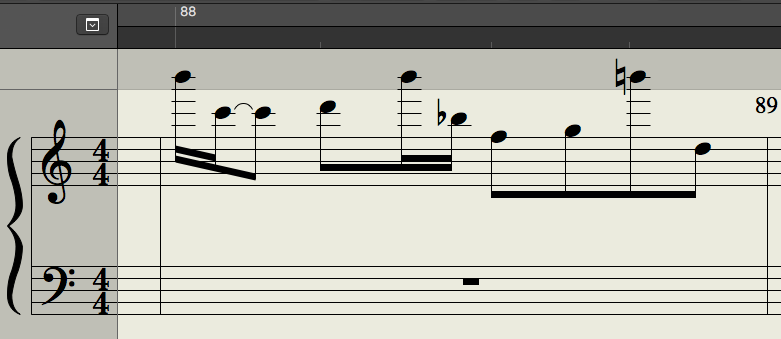
\includegraphics[scale=0.5]{images/pieciolinia_logic.png}
    \caption{Przykład notacji muzycznej wygenerowanej z pliku MIDI w programie Logic Pro X. Widać na nim takie informacje jak metrum czy wysokości i długości granych dźwięków}
  \end{center}
\end{figure}




\subsection{Rytm} \label{sec:rytm}
W kontekście muzykologii, rytm jest relacją czasową pomiędzy poszczególnymi dźwiękami, tworzącą strukturę rytmiczną utworu. Nie można niestety zakładać stałości rytmu na przestrzeni całej kompozycji, ponieważ powszechną praktyką kompozytorów jest jego modyfikacja na przestrzeni piosenki w celu uzyskania konkretnych efektów artystycznych. Dla przykładu, minimalne podnoszenie tempa na czas każdego z refrenów jest powszechnie stosowane w muzyce popularnej.

Informacja o rytmie jest zapisana w relacjach pomiędzy poszczególnymi dźwiękami i pomiędzy większymi strukturami wewnątrz utworu. Odstęp pomiędzy początkami dźwięków (\textit{ang. Inter-onset interval, IOI}) pełni bardzo istotną rolę w rytmice utworu, jak i strukturze perkusyjnej. Pojęcie to odnosi się do interwału czasowego pomiędzy dwoma początkami dźwięków (np. moment uderzenia w werbel), która to cecha jest dużo bardziej istotna w rytmice niż długość danych dźwięków 
\cite[482-489]{Transcription:Clarke:RhythmAndTiming}
%\cite[r. 4]{Transcription:Clarke:RhythmAndTiming}
.

Podstawową jednostką rytmiczną jest nuta. Miarą tempa utworu przeniesioną na domenę fizyczną są \textit{uderzenia na minutę} \textit{(ang. beats per minute, BPM)} oznaczające liczbę ćwierćnut (beatów) przypadających na jedną minutę. \textit{Taktem} nazywamy odcinek zapisu muzycznego wizualnie oznaczony pionowymi kreskami. Takty tworzą regularne odcinki czasowe, a ich długość jest zależna od \textit{metrum}. Metrum jest oznaczeniem metrycznym opisującym ile jakich jednostek mieści się w takcie. Dla przykładu, najpopularniejszym metrum w muzyce pop jest 4/4, co oznacza, że w każdym takcie mieszczą się cztery ćwierć nuty.

\begin{figure}[H]
  \begin{center}
    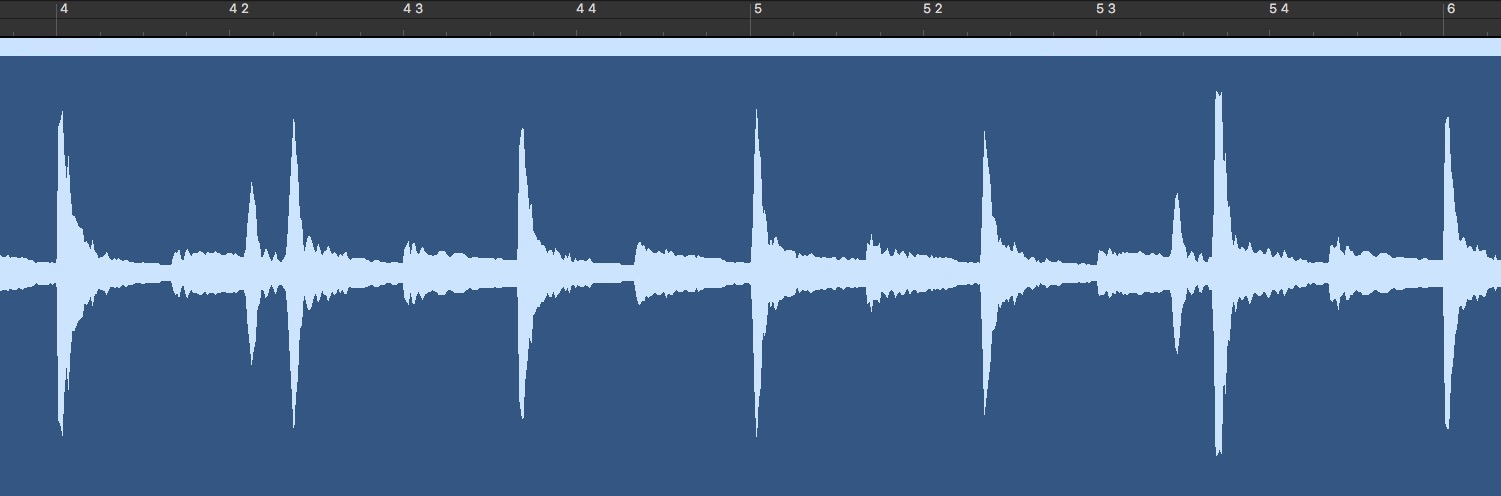
\includegraphics[scale=0.3]{images/RythmMertic.jpg}
    \caption{Sygnał akustyczny z wyraźnymi metrykami muzycznymi. Na osi poziomej liczbowo oznaczona jest metryka nutowa (4 beaty), mniejszymi zaś regularne odstępy taktowe.}
    \label{fig:rythmMertic}
  \end{center}
\end{figure}

Zbadanie rytmiki wymaga wyznaczenia metrum i długości poszczególnych jednostek metrycznych utworu. Ze względu na to, że nagrania muzyczne cechują się periodycznością wokół tych jednostek, wykrycie wzorca regularnych, przeplatanych akcentowanych i nieakcentowanych uderzeń (często nazywanych słabszymi i silniejszymi) 
\cite[12-35]{Transcription:Lerdahl:GenerativeTheory}
%\cite[r. 2]{Transcription:Lerdahl:GenerativeTheory}
. Pozyskane \textit{pulsy} o różnych czasowych poziomach razem tworzą strukturę rytmiczna. Przykład takiej struktury przedstawiony jest na rysunku \ref{fig:rythmMertic}, który przedstawia sygnał nagranej perkusji. W równych odstępach pojawiające się piki oznaczają stopkę, werbel oraz talerze, każde występują okresowo.

W skład rytmu wchodzi również \textit{grupowanie}. Termin ten odwołuje się do powiązań pomiędzy pojedyńczymi dźwiękami, które razem tworzą łączne frazy, a te z kolei dalej grupowane tworzą większe i bardziej złożone jednostki w hierarchicznej strukturze 
\cite[12-35]{Transcription:Lerdahl:GenerativeTheory}
%\cite[r. 2]{Transcription:Lerdahl:GenerativeTheory}
.

\subsection{Wysokość tonu}\label{sec:pitch}
Wysokość tonu, czy też wysokość dźwięku, jest percepcyjnym atrybutem za pomocą którego porządkowane są dźwięki na skali częstotliwości, od najniższych do najwyższych. Jest to pojęcie tożsame z częstotliwością sygnału sinusoidalnego zgodnego z tym, które jest rejestrowane przez ludzkie ucho 
\cite[3492-3493]{Transcription:Hartmann:PitchPeriodicityAuditoryOrganization}
%\cite[sekcja 2]{Transcription:Hartmann:PitchPeriodicityAuditoryOrganization}
. 

\begin{figure}[H]
  \begin{center}
    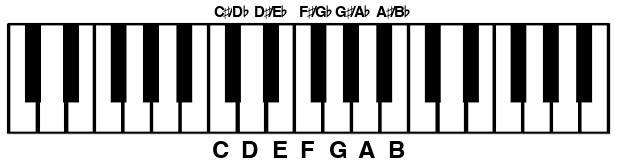
\includegraphics[scale=0.5]{images/PianoRoll.png}
    \caption{Ilustracja przedstawiająca trzy oktawy klawiatury pianina z oznaczonymi muzycznymi nazwami nut}
    \label{fig:pianoRoll}
  \end{center}
\end{figure}

\textit{Częstotliwość fundamentalna} (w dalszej części oznaczana jako \textit{F0}) jest terminem fizycznym dla sygnałów okresowych i prawie okresowych zdefiniowany jako odwrotność długości okresu sygnału. W niejednoznacznych przypadkach F0 określony jest jako okres odpowiadający postrzeganej wysokości tonu 
\cite[8]{Transcription:Anssi:SignalProcessingMethods}
%\cite[r. 1.1]{Transcription:Anssi:SignalProcessingMethods}
.

F0 jest ściśle powiązana z wysokością tonu. Współczesna muzyka zachodnia opera się na \textit{skali melowej}. System równomiernie poddaje nuty kwantyzacji na logarytmicznej skali spektrum częstotliwości na tak zwane półtony, czyli najmniejsze interwały. Każda z tak powstałych muzycznych nut ma przypisaną literę w celu odróżnienia, alfabetycznie od A do G wraz razem z podwyższeniami (moll, w języku angielski \textit{sharp} oznaczany symbolem $\sharp$) i obniżeniami (dur, w języku angielskim \textit{flat} oznaczany symbolem $\flat$) półtonowymi. Tak nazwane wysokości są grupowane w oktawy, z których każda zawierająca 12 półtonów. Pełna nazwa granego dźwięku powinna zawierać nazwę literalną wraz z numerem oktawy. Ze względu na tak skonstruowany system nazewnictwa, niektóre z dźwięków mogą mieć dwie poprawne nazwy (np. A$\sharp$4 i B$\flat$4). O tym, którą z tych dwóch nazw należy użyć, zazwyczaj zależy konwencja którą używa kompozytor 
\cite[215-220]{Transcription:Burns:InversalScalesTuning}
%\cite[r. 7.2]{Transcription:Burns:InversalScalesTuning}
.

Omówiony system zakłada referencyjne mierzenie częstotliwości zależnie od wysokości A4, która powinna być równa 440 Hz. Każda podwyższenie oktawy powinno powodować dwukrotne zwiększenie sie częstotliwości fundamentalnej. Standard MIDI mapuje daną częstotliwością bazową na liczbę rzeczywistą odpowiadającą wysokości dźwięku przy pomocy wzoru 
\cite[67-71]{Homerecording:LevelUp}
%\cite[r. 2]{Homerecording:LevelUp}
:
\begin{equation} \label{eq:midi_freq}
p = 69 + 12 * \log{2}(\frac{f}{440 Hz})
\end{equation}

Istnieją oczywiście instrumenty, które generują dźwięki o dowolnej częstotliwości fundamentalnej, a nie jedynie o dyskretnej wartości, jak na przykład skrzypce czy saksofon. Kwantyzacja wysokości dźwięku jest procesem, który kategoryzuje dźwięki do najbliższej wartości w sensie częstotliwości nazwanych nut, dzięki czemu można je formalnie zapisać w procesie transkrypcji.

Interesującą własnością niemalże wszystkich kultur muzycznych jest podobieństwo do siebie odpowiednich nut w oktawach. Nuty A2, A3 i A4 dla przykładu mają taką samą rolę w kontekście harmoniczności. Brzmią one bardzo podobnie do siebie, jedynie różnią się wysokością. Ze względu na tą cechę, opisany wyżej system redukuje liczbę wszystkich istniejących dźwięków do jedynie 12 klas dźwięków, po 1 na każdą z nut w oktawie. Korzystając ze wzoru ~\ref{eq:midi_freq} dla wielokrotności liczby 440 można uzyskać tabelkę z częstotliwościami dźwięków \textit{A} w kolejnych oktawach, jak w tabeli \ref{tab:FqMidi}.

\begin{table}[ht]
  \begin{center}
    \begin{tabular}{ |c|c|c| } 
    \hline
    p & f & Literalna nazwa wysokości dźwięku\\
    \hline
    33 & 55 & A1\\
    45 & 110 & A2\\
    57 & 220 & A3\\
    69 & 440 & A4\\
    81 & 880 & A5\\
    93 & 1760 & A6\\
    105 & 3520 & A7\\
    \hline
    \end{tabular}
  \end{center}
  \caption{Wysokości kolejnych dźwięków A zgodna ze wzorem ~\ref{eq:midi_freq}}
  \label{tab:FqMidi}
\end{table}

Relacja pomiędzy wysokościami używanych tonów jest ważną informacją przy analizie muzycznej. Mimo dużej ilości możliwych częstotliwości, używane nuty często ograniczane są do podzbiorów według tak zwanych kluczy. Badając rozkład częstotliwości takie informacje mogą znacznie ograniczyć błędy podczas badania sygnału. Należy jednak mieć na uwadze fakt, że nagrany instrument może nie posiadać dokładnie takiej samej częstotliwości jak oczekiwana dla danej wysokości tonu ze względu na charakterystykę instrumentu czy też techniczne parametry nagrania. Dodatkowym utrudnieniem są skale które bazują na innych niż zachodnich systemach dobierania wysokości. W tej pracy badane będą jedynie utwory bazujące na wyżej opisanym systemie, jednak na uwadzę należy mieć fakt, że nie jest to uniwersalne rozwiązanie. Również z artystycznych względów docelowe częstotliwości generowane przez instrumenty odbiegają od tych przewidzianych przez opisany system. Nieharmoniczność najczęściej ustala się na poziomie 5\%, lecz nie istnieje sformalizowany zakres. Próba rozpoznawania jedynie konkretnych częstotliwości tonów mogło by być dużym uproszczeniem w analizie sygnałów fonicznych, lecz jednocześnie znacząco ograniczyłby jej uniwersalność 
\cite[64-65]{Homerecording:DlaKazdego}
%\cite[r. 2]{Homerecording:DlaKazdego}
 \cite[7-11]{Transcription:Anssi:SignalProcessingMethods}
% \cite[r. 1.1]{Transcription:Anssi:SignalProcessingMethods}
 .

\subsection{Głośność} \label{sec:loudness}
Termin głośności z reguły nie odnosi się do pojedyńczych nut, ale do większych sekcji. W notacji muzycznej nie często używa się słowa ,,głośność''. To co słuchacz odbiera jako siłę dźwięku z punktu widzenia muzyka jest dynamiką granego fragmentu. Większość instrumentów używanych do tworzenia muzyki posiada zdolność wytworzenia zróżnicowanych w sile fal akustycznych. Podstawą skali dynamiki są dwa słowa kluczowe:

\begin{itemize}
  \item \textbf{f} (forte) - głośno
  \item \textbf{p} (piano) - cicho
\end{itemize}

Pomiędzy wymienionymi stopniami istnieją kroki pośrednie, odpowiednio mezzo\-forte (dość głośno) i mezzo-piano (dość cicho). Poza czterema wymienionymi przypadkami dostępne są również skrajności odpowiadające za bardzo głośny (odpowiednio - cichy) i możliwie najgłośniejszy (odpowiednio - najcichszy) odcień dynamiki.

Z punktu widzenia algorytmicznej analizy muzyki problematyczne są dynamiki zwane crescendo i diminuendo. Odpowiadają one za kolejno stopniowe wzmacnianie i stopniowe osłabianie natężenia dynamiki. Łatwo jest pomylić takie zabiegi z innymi cechami sygnału audio.

Warto też wspomnieć o technice zwanej \textit{tremolo}, która określa artykulacje  grania wielu dźwięków o tej samej wysokości z różną dynamiką. Analizując sygnał łatwo jest pomylić kolejne uderzenia tremolo z zagraniem nowych nut.

Z praktycznego punktu widzenia głośność w plikach muzycznych jest zdeterminowana przez to, jak dany utwór został wyprodukowany. W procesie nagrywania ogromne znaczenia ma położenie i rodzaj mikrofonu, jak i otoczenie w którym rejestrowany jest dźwięk. Mikrofony posiadają różne pasma przenoszenia i charakterystyki kierunkowe, które nie tylko mogą zniekształcić głośność nagrywanego instrumentu, ale również jego barwę. Różne rodzaje mikrofonów są wykorzystywane przy różnych źródłach dźwięku, np. mikrofony pojemnościowe są odpowiedniejsze do nagrywania wokali i instrumentów akustycznych niż wstęgowe, ponieważ przenoszą częstotliwości tych właśnie źródeł bardziej wiarygodnie 
\cite[48-52]{Homerecording:DlaKazdego}
%\cite[r. 1]{Homerecording:DlaKazdego}
. Charakterystyka niektórych powierzchni może sprawić, że fałszywie cichsze częstotliwości będą wychodziły na przód nagrania. Mocna kompresja dynamiki utworu jest powszechna praktyką podczas procesu miksowania i masterowania utworów. Dzieje się tak, ponieważ ludzie impulsywnie uważają głośniejsze utwory za lepsze, co doprowadziło rynek muzyczny do produkowania utworów o niemal stałej dynamice głośności, co mogło graniczyć z białym szumem. Choć temat ten jest w trakcie regulacji, przez między innymi wprowadzenie ograniczeń dynamiki na podstawie jednostki LUFS danego utworu, dokładne analizowanie głośności wielu istniejących nagrań może doprowadzić do nieprawdziwych wniosków.

\begin{figure}[H]
  \begin{center}
    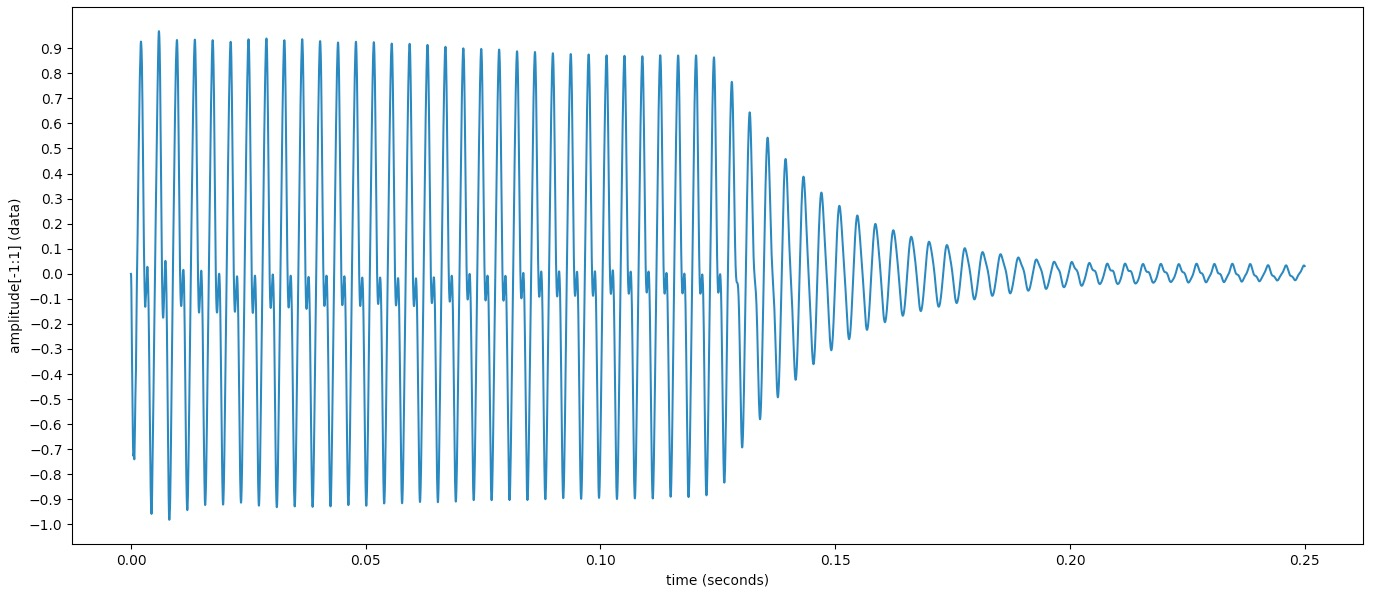
\includegraphics[scale=0.32]{images/Amplitude.jpg}
    \caption{Wykres przedstawiający sygnał dźwięku o zmiennej amplitudzie (głośności) względem czasu wygenerowany przez klasyczne pianino elektryczne.}
    \label{fig:amplitude}
  \end{center}
\end{figure}

\subsection{Barwa dźwięku}\label{sec:barwaDzwieku}
Barwa dźwięku (inaczej tembr) jest cechą odwołującą się do harmonicznej domeny sygnału fonicznego. Pozwala ona na odróżnienie od siebie dźwięków o tej samej głośności i wysokości granych na różnych instrumentach. Silne tony harmoniczne danej barwy sprawiają, że dźwięk jest bardziej wyrazisty. W przeciwnym wypadku, gdy siła tonów harmonicznych jest mała, sygnał staje się bardziej rozmyty dla odbiorcy. Barwa dźwięku jest zależna od amplitudy poszczególnych tonów harmonicznych, ich rozkładu w widmie jak i samej struktury tego widma. Jest to dobrze widoczne na rysunku \ref{fig:spektrogram}.

\begin{figure}[t]
  \begin{center}
  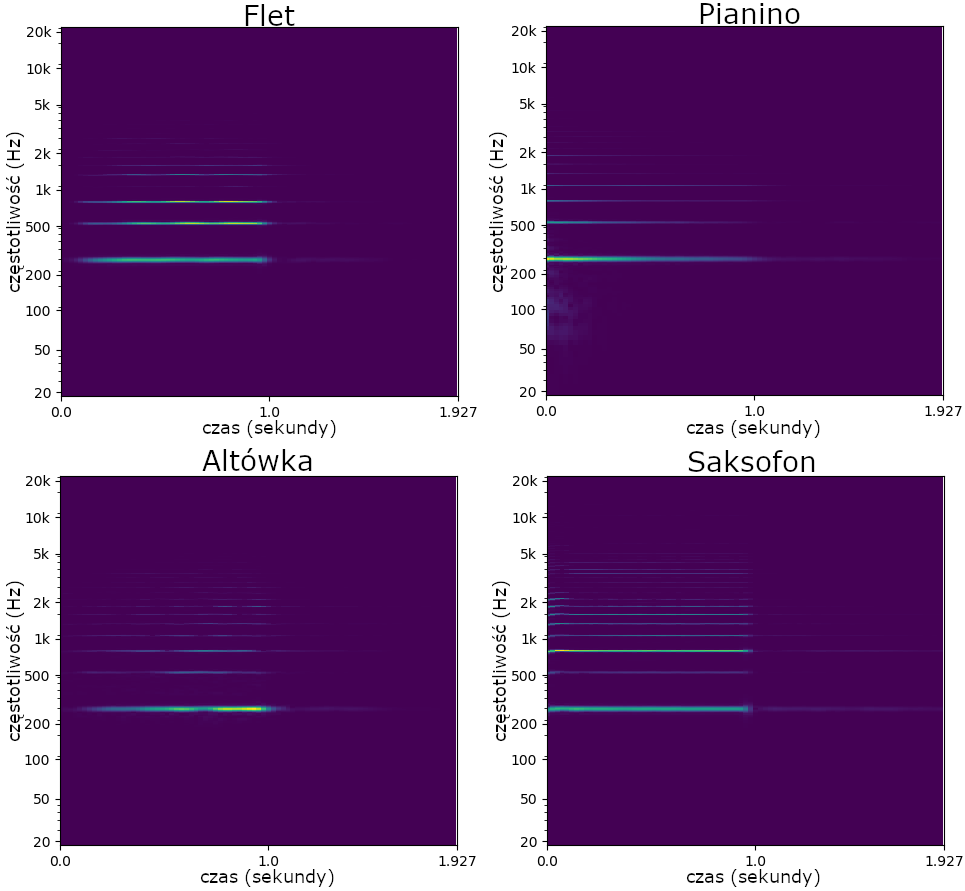
\includegraphics[scale=0.4]{images/spectogram_instruments.png}\\
  \caption{Spektrogramy dźwięku C3 (130.81Hz) grane na czterech różnych instrumentach (flet, pianino, altówka i saksofon) pokazują różnice w ilości i rozmieszczeniu harmonicznych każdego z dźwięków. Spektrogramy wykonane z 4096 samplami na okno, odstępem okien 1024 sampli i funkcją okna Hanna. Jaśniejsze obszary symbolizują większą magnitudę.}
  \label{fig:spektrogram}
  \end{center}
\end{figure}

Ułożenie tonów harmonicznych jest zintegrowane z harmonią pomiędzy różnymi granymi nutami. Gdy dwa dźwięki są grane w tym samym czasie, nakładające się na siebie harmoniczne sprawiają, że dźwięk brzmi pozornie spójnie. Generuje to dodatkowe komplikacje dla algorytmów wykrywających wysokość tonów, które muszą odseparować nakładające się na siebie nuty.

Barwa dźwięku nie jest stała w czasie. Harmoniczne o wysokich częstotliwościach szybciej cichną w porównaniu do tych o niższych. Powoduje to, że nie tylko średnia głośność jest mniejsza, ale także barwa ulega modyfikacji. Dla instrumentów dętych czy skrzypiec cechy jak wysokość tonu, głośność i barwa pozostają relatywnie stałe przez cały okres grania nuty, natomiast dźwięk pianina ,,rozmywają'' się w czasie przez ich zmienną barwę. Ta cecha barwy dźwięku musi zostać zaadresowana przy próbie dokładnej analizy sygnału fonicznego 
\cite[64-65]{Homerecording:DlaKazdego}
%\cite[r. 2]{Homerecording:DlaKazdego}
 \cite[804–805]{Transcription:Klapuri:MultipleFundamentalFrequencyEstimation}
% \cite[sekcja 1]{Transcription:Klapuri:MultipleFundamentalFrequencyEstimation}
 .

Istotnym pojęciem przy omawianiu barwy dźwięku jest \textit{formant}. Formantem nazywane jest pasmo częstotliwości, w którego obrębie częstotliwości harmoniczne są wzmocnione względem pozostałych częstotliwości danego sygnału. Formanty mogą sprawić, że harmoniczne będą miały większą amplitudę niż częstotliwość fundamentalna. Istnienie tego zjawiska fonicznego uniemożliwia poprawność podejścia, w którym jako częstotliwość fundamentalna wybierana była by ta, o największej amplitudzie w analizowanym oknie 
\cite[24-25]{Transcription:Klapuri:Phd}
%cite[r. 3.3.1]{Transcription:Klapuri:Phd}
.
\newpage
\section{Modelowanie systemu transkrypcji} \label{sec:modelowanieSystemu}
Sygnały akustyczne, przetworzone przez przetwornik analogowo-cyfrowy (A/C) są przechowywane w postaci binarnych plików dźwiękowych jako dyskretne sygnały cyfrowe dyskretnego czasu. W procesie cyfryzacji zostały poddane procesowi kwantyzowania wartości, najczęściej poprzez zaokrąglenie do najbliższych liczb całkowitych 
\cite[1-4]{CyfrowePrzetwarzanieSygnalowOdTeoriiDoZastosowan}
% \cite[r. 1.1-1.2]{CyfrowePrzetwarzanieSygnalowOdTeoriiDoZastosowan}
. Sposób, w jaki pliki te przechowują dane jest zdeterminowany przez wiele parametrów, jak kodowanie, które zostało na nich zastosowane, częstotliwość próbkowania, ilość kanałów itp. Istnieje wiele kodowań przeznaczonych do danych dźwiękowych, zarówno nieskompresowanych jak i skompresowanych. Te drugie powstały z myślą o zaoszczędzeniu jak największej ilości pamięci w znaleźć od tego, w jakim stopniu można obniżyć jakość podczas kompresji sygnału 
\cite[66]{Homerecording:DlaKazdego}
%\cite[r. 2]{Homerecording:DlaKazdego}
. Częstotliwość próbkowania ma również znaczący wpływ na wynikowy rozmiar plików, jak i ilość bitów przeznaczony na pojedyńczy sampel. Wszystkie cechy jakie posiada cyfrowa reprezentacja rzeczywistego dźwięku muszą być wzięte pod uwagę podczas jej przetwarzania.

W kontekście algorytmów generujących muzykę, binarne pliki dźwiękowe nie posiadają efektywnej struktury pozwalającej na trzymanie akustycznych informacji o melodii czy rytmice. Cechy, które można wydobyć ze zdigitalizowanego strumienia audio mogą posłużyć za istotne wskaźniki przy klasyfikacji zbiorów, natomiast kluczowe informacje odnoszące się do struktury kompozycji i harmonii poszczególnych sekcji szukać należy w transkrypcji danego utworu. 

Utwór muzyczny posiada bardzo wiele własności na podstawie których można opierać analizę. W celu zoptymalizowania algorytmu automatycznej transkrypcji należy przefiltrować wszystkie te dane i zdecydować się, które uznać za istotne, a które można uznać za zaniedbywalne. Strukturyzacja algorytmu i dobór reprezentacji danych jest równie istotna przy projektowaniu algorytmu.

Neuropsychologiczne badania, które były prowadzone w kontekście przetwarzania muzyki przez ludzki umysł dowodzą, że analiza dźwięku jest dzielona na pod-zadania. Jak opisują autorzy w \cite{Transcription:Zatorre:AuditoryCortex} pewne własności muzyki są przez mózg odseparowywane od reszty bez szerszego kontekstu. Daje to informacje o tym, że modularyzacja podejścia do transkrypcji może być właściwym rozwiązaniem tego problemu. W automatycznej transkrypcji muzyki często używa się innych reprezentacji danych do analizy wysokości dźwięku, w których większy nacisk kładzie się na wierne odwzorowanie częstotliwości, a innych do analizy rytmu, w których najważniejsze jest dokładność w domenie czasu 
\cite[11-13]{Transcription:Anssi:SignalProcessingMethods}
%\cite[r. 1.2.1-1.2.2]{Transcription:Anssi:SignalProcessingMethods}
.

W pracy naukowej 
\cite[22-24]{DBLP:journals/spm/BenetosDDE19}
%\cite[sekcja pt. "An overview of AMT methods"]{DBLP:journals/spm/BenetosDDE19}
 autorzy opisują obecny stan nauki w dziedzinie transkrypcji muzyki, i kategoryzują oni algorytmy AMT ze względu na poziom abstrakcji używanych struktur na cztery kategorie:
\begin{itemize}
  \item transkrypcje na poziomie okien czasowych, badając każde okno osobno w poszukiwaniu kandydatów F0. Algorytmy na tym poziomie wykorzystują między innymi tradycyjne metodyki przetwarzania sygnału, modelowanie probabilistyczne, podejścia bayesowskie, nieujemna faktoryzacja macierzy (NMF, z ang. \textit{non-negative matrix factorization}) i sieci neuronowe (NN, z ang. \textit{Neural Network}). Ta praca skupia się na tradycyjnym przetwarzaniu sygnału z elementami podejścia bayesowskiego (\ref{sec:f0}, \ref{sec:pertus1}) ale opisana jest również sieć neuronowa wykazująca najlepsze do tej pory rezultaty (\ref{sec:multif0:onsetsAndFrames}).
  \item transkrypcje na poziomie nut, zwane też śledzeniem wysokości. W odróżnieniu od poziomu okien czasowych, w tym podejściu analizowane są sąsiednie wyniki w celu połączenia ich w spójne muzycznie całości. Przykład tego podejścia opisany jest w \ref{sec:petrus2}.
  \item transkrypcje na poziomie strumienia, zwana także strumieniowaniem wielotonowym (MPS, z ang. \textit{Multi-Pitch Streaming}), które grupuje nuty wydobyte z poziomu nut w strumienie, najczęściej odpowiadające charakterystyce źródła fali akustycznej (odpowiadające instrumentowi).
  \item transkrypcje na poziomie notacji muzycznych. Jest to poziom najmniej zbadany na ten moment. Jego celem jest wygenerowanie transkrypcji w postaci czytelnej dla człowieka. Poziom ten zakłada wydobycie informacji  o strukturach muzycznych, które nie są istotą analizy pozostałych algorytmów. Przykład takiej analizy jest opisany w \ref{sec:multif0:petrusNetwork} przy użyciu sieci neuronowych.
\end{itemize}


\subsection{Reprezentacja danych średniego poziomu}
Koncepcja pojęcia \textit{Reprezentacja danych średniego poziomu} pozwala na utworzenie pewnego rodzaju pośrednika pomiędzy akustyczną reprezentacją dźwięku, a tą formalnie zapisaną. Sygnał muzyczny w czystej postaci jest mało informatywny, nie możemy z niego wyczytać chociażby poszczególnych nut utworu, tak jak jest to widoczne w zapisie nutowym. W książce 
\cite[13-17]{Transcription:Anssi:SignalProcessingMethods}
%\cite[r. 1.2.3]{Transcription:Anssi:SignalProcessingMethods}
 autorzy sugerują, że celem użycia tego narzędzia jest stworzenie pośredniego stopnia abstrakcji, które będzie działało jak interfejs do analizy audio i do ułatwienia konstrukcji systemów transkrypcji.

Najczęściej używaną reprezentacją danych na średnim poziomie przy analizie sygnału akustycznego jest szybka transformacja Fouriera (dokładniej opisana w sekcji \ref{sec:FFT}) sygnału w kolejnych oknach czasowych. W ogólności wszystkie funkcje pozwalające na przeniesienie sygnału z domeny czasowej na domenę częstotliwości są niezwykle istotne w analizie dźwięku. W tej pracy znajduje się opis algorytmów operujących na tej właśnie reprezentacji danych (analiza tej reprezentacji opisana jest w sekcji \ref{sec:f0:tfr}, algorytmy jak ACLOS opisany w sekcji \ref{sec:f0:aclos} czy cepstrum opisane w \ref{sec:f0:ceps} działają jedynie na widmie sygnału).

W książce 
\cite[13-17]{Transcription:Anssi:SignalProcessingMethods}
%\cite[r. 1.2.3 - 1.2.5]{Transcription:Anssi:SignalProcessingMethods}
 autorzy uważają, że powszechnym wyborem dla reprezentacji danych na średnim poziomie jest bazowanie na \textit{ścieżkach sinusoidalnych}. W tym przypadku sygnał akustyczny jest przedstawiony jako suma sinusoid o zmiennych w czasie częstotliwościach i amplitudach. Korzyścią, jaka płynie z tej reprezentacji jest łatwe przedstawienie instrumentów tonalnych. Problem z tym podejściem zaczyna się przy wielotonalnych sygnałach, gdzie dźwięki nakładają się na siebie w domenie częstotliwości i czasu. 

Modele bazujące na słuchu człowieka są również używane jako reprezentacje danych na średnim poziomie. Sposób w jaki ludzki mózg przetwarza muzykę jest w zasadzie tym, co jest istotą transkrypcji, więc naturalnym wydaje się próba naśladowania procesów neuronowych. Sposób ten ma podłoże neuropsychologiczne. Dokładne opisy modeli słuchowych znajdują się w pracach \cite{Transcription:Karjalainen:MultipitchAnalysisModel} czy \cite{Transcription:Zatorre:AuditoryCortex}.

Nie ma jednoznacznej reguły, która decydowałaby o trafności reprezentacji danych na średnim poziomie. Dobór metody powinien być świadomy, zgodny z wymaganiami systemu transkrypcji w którym reprezentacja ma zostać użyta 
\cite[13-15]{Transcription:Anssi:SignalProcessingMethods}
%\cite[r. 1.2.3]{Transcription:Anssi:SignalProcessingMethods}
. Różnice w reprezentacjach można zaobserwować na wykresach na rysunku \ref{fig:mid_level_representation}. 

\begin{figure}[t]
  \begin{center}
  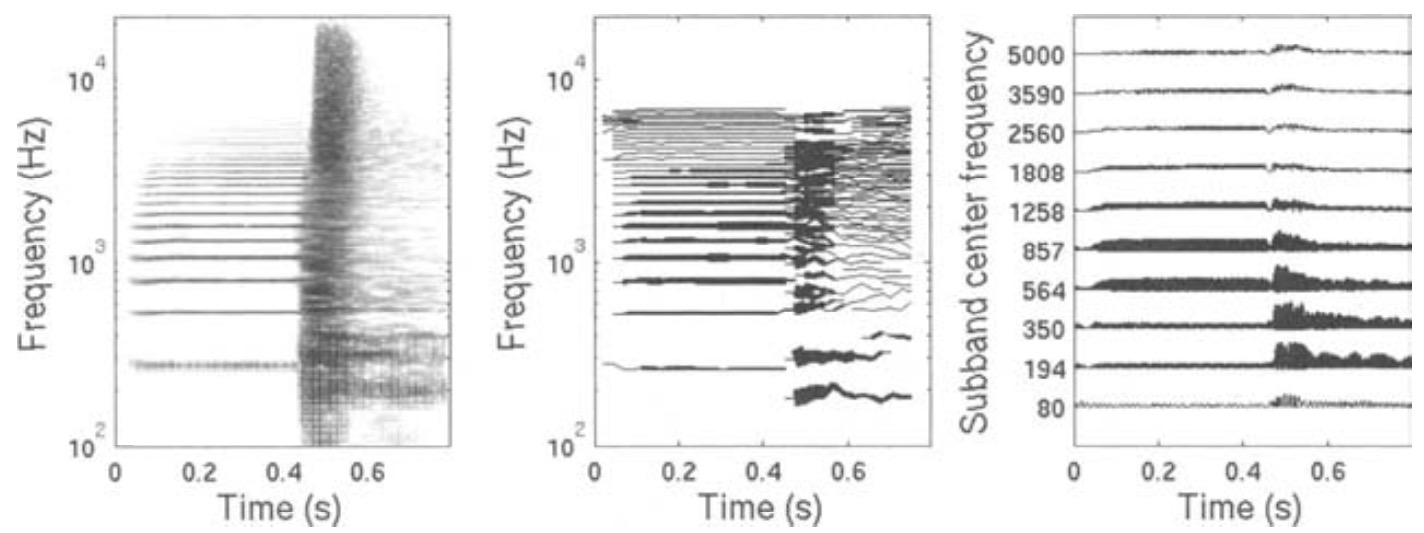
\includegraphics[scale=0.3]{images/mid_level_representation.jpg}\\
  \caption{Grafy przedstawiają 3 różne reprezentacje danych na średnim poziomie tego samego dźwięku trąbki grającej dźwięk C4. Lewy wykres przedstawia spectrogram na logarytmicznej skali częstotliwości. Środkowy wykres przedstawia reprezentację ścieżek sinusoidalnych, przy czym szerokość lini oznacza amplitudę poszczególnych sinusoid. Prawy wykres przedstawia prosty model słuchowy. Wykres z 
  \cite[14]{Transcription:Anssi:SignalProcessingMethods}
  %\cite[r. 1.2.3]{Transcription:Anssi:SignalProcessingMethods}
  }
  \label{fig:mid_level_representation}
  \end{center}
\end{figure}

\subsection{Transformata Fouriera}\label{sec:TF}
Pliki dźwiękowe zawierają informacje, które reprezentują siłę ciśnienia akustycznego w domenie czasu. Jest to jedna z reprezentacji, która może być analizowana w celu zbadania konkretnych cech sygnału, lecz jest ona bezpośrednim efektem nagrania muzyki i możliwości jej bezpośredniego odtworzenia. Dokładna analiza relacji sygnału muzycznego, jego reprezentacja jak i jego zrozumienie odbywa się po przeniesieniu na płaszczyznę częstotliwości. W muzyce zachodniej, F0 w zapisie nutowym definiuje się jako wysokość dźwięku w rozumieniu częstotliwości, co zostało po omówione w sekcji \ref{sec:pitch}.

Aby z sygnału akustycznego w domenie czasu uzyskać dane w domenie częstotliwości powszechnie używane jest narzędzie matematyczne o nazwie \textbf{transformata Fouriera}. Funkcja ta jest uniwersalna i powszechnie stosowana w analizie sygnałów, w tej pracy jednak skupię się się na opisaniu sposobów wykorzystywania jej do celów analizy sygnałów akustycznych. Transformata ta opiera się na założeniu, że każdą okresową krzywą można zapisać w postaci sumy składowych sinusoidalnych o różnych częstotliwościach. Funkcja ta przekształca sygnału z dziedziny czasu na dziedzinę częstotliwości, co daje zarys tego jak rozłożona jest częstotliwość poszczególnych częstotliwości w analizowanych danych. Transformata zadana jest wzorem:

\begin{equation} \label{eq:fourier-base}
CFT_x(f) = X(f) = \int_{-\infty}^{\infty}\textit{f}(t)e^ {-j2\pi ft}\mathrm{d}t
\end{equation}
Gdzie F(f) nazywane jest transformatą Fouriera f(t) lub widmem częstotliwościowym. Wynik transformaty jest listą liczb zespolonych, dzięki czemu można ją odwrócić przy pomocy odwrotnej transformaty Fouriera (IFT, ang. \textit{Inverse Fourier Transformation}) opisanej wzorem:

\begin{equation} \label{eq:inverse:fourier-base}
ICFT_x(f) = \int_{-\infty}^{\infty}\textit{F}(t)e^ {j2\pi ft}\mathrm{d}t = x(t)
\end{equation}
\cite{TransformacjaFourieraWroc}\cite{TransformacjaFourieraAgh}
\cite[22-25]{Transcription:Anssi:SignalProcessingMethods}
%\cite[r. 2.1.1 - 2.1.2]{Transcription:Anssi:SignalProcessingMethods}
.

Do analizy całego spektrum utworu muzycznego, pojedyńcza transformata Fouriera może nie być wystarczająca ze względu na długość i zróżnicowanie utworu względem czasu. Reprezentacja czasu-częstotliwości pozwala na przedstawienie sygnału w postaci zespolonej w domenie czasu i częstotliwości (ang. time–frequency representation, TFR). W celu uzyskania takiej reprezentacji przy pomocy FT z zastosowaniem okna czasowego, co jest szerzej opisane w sekcji \ref{sec:STFT}. Okna te pełnią rolę prostego TFR, spektrogramu jak i reprezentację czasową czy reprezentację opóźnienia czasowego 
\cite[21-23]{Transcription:Anssi:SignalProcessingMethods}
%\cite[r. 2.1.1]{Transcription:Anssi:SignalProcessingMethods}
.

\subsubsection{Dyskretna transformata Fouriera} \label{sec:DFT}
Jednym z założeń transformacji Fouriera jest aby f(t) z \ref{eq:fourier-base} była funkcją ciągłą na przedziale od minus nieskończoności do nieskończoności, co przekłada się na transformatę w tym właśnie zbiorze. Z praktycznego punktu widzenia nieskończone granice sumy są niemożliwe do zrealizowania w analizie sygnału akustycznego, ponieważ przetwarzane są tylko skończone długości krzywych, co powoduje, że granice są zawsze skończone. W celach analitycznych na sygnałach, zwłaszcza w kontekście transkrypcji muzyki, dane brane pod uwagę są brane z ograniczonego przedziału czasowego. Potrzebne do tego celu będzie podzielenie analizowanych danych na krótkie próbki \cite{TransformacjaFourieraWroc}\cite{TransformacjaFourieraelektronikab2b}.

\textbf{Dyskretna transformata Fouriera (DFT)} jest narzędziem matematycznym analogicznym do podstawowej transformaty Fouriera, lecz przeznaczonym do analizowania sygnału dyskretnego $x(n)$ o okresie $N$, opisanego następującym wzorem:
\begin{equation} \label{eq:DFT-periodicy}
  x(n) = x(n + mN)
\end{equation}
Pozwala ona na analizę pojedyńczego okresu zadanego sygnału. Własność ta jest szczególnie przydatna przy komputerowej analizie sygnałów, w tym fonicznych. Jest to transformacja zawsze odwracalna. 

DFT zakłada wyznaczenie iloczynu sygnału i okna prostokątnego (o którym więcej znaleźć można w sekcji \ref{sec:STFT}), które to jest wycinkiem krzywej sygnału podlegającym analizie. W związku z cyklicznością zakładanego sygnału (\ref{eq:DFT-periodicy}) przyjmuje się, że analizowany sygnał jest okresowy z okresem równym $N$, co implikuje obliczenie dokładnie N składowych harmonicznych analizowanych danych (N różnych częstotliwości). Dyskretny czas, częstotliwość i skończona liczba próbek zadanego sygnału sprowadza omawianą transformacje do funkcji w pełni dyskretnej. Wynik dyskretyzacji TF jest następujące równanie:
\begin{equation} \label{eq:DFT}
  DFT_x(k) = X(k) = \sum_{n = 0}^{N-1} x(n)e^{-j{2 \pi}kn},  k = 0, 1, 2,..., N-1
\end{equation}
DFT, tak samo jak FT jest odwracalna, co można opisać wzorem:
\begin{equation} \label{eq:IDFT}
  IDFT_x(n) = \sum_{k = 0}^{N-1} X(k)e^{j2\pi kn} = x(n), n = 0, 1, 2,..., N-1
\end{equation}
Wynikiem transformacji będzie N liczb odpowiadających kolejno amplitudzie i fazie sinusoid od $- \frac{1}{2} \Delta $ do $\frac{1}{2} \Delta $, gdzie $\Delta$ jest częstotliwością próbkowania, w rozdzielczości $\frac{1}{N} \Delta$. Częstotliwości są ustalone przez częstotliwość próbkowania oraz liczbę próbek w oknie. Jak opisuje Tomasz Zieliński w 
\cite[198 - 200, 204-206]{CyfrowePrzetwarzanieSygnalowOdTeoriiDoZastosowan}
%\cite[r. 8.1.4, r. 8.2]{CyfrowePrzetwarzanieSygnalowOdTeoriiDoZastosowan}
, DFT stanowi pewną aproksymację $N$-elementowego wektora próbek analizowanego sygnału za pomocą $N$ ortogonalnych wektorów bazowych $N$-elementowych, z wyjątkiem sytuacji, kiedy w sygnale występuje składowa sinusoidalna, która nie jest częścią zbioru wektorów bazowych, bo w takim wypadku zostanie ona przedstawiona jako suma większej liczby sygnałów ,,bazowych'', co oznacza, że jej widmo ulegnie rozmyciu.

\subsubsection{Szybka transformacja Fouriera} \label{sec:FFT}
DFT omawiana w sekcji \ref{sec:DFT} jest wystarczająca do wykonania wszelkich analitycznych przekształceń. Problem jednak pojawia się w praktyce, i jest nim efektywność algorytmu. W swojej czystej formie transformata Fouriera $F_n$ wymaga zliczenia wszystkich wartości od $h_0$ do $h_{N-1}$ dla każdej z częstotliwości $n$, co oznacza, że złożoność obliczeniowa dla N danych wynosi $O(N^2)$, co jest zbyt dużym obciążeniem nawet dla najlepszych pod względem mocy obliczeniowej współczesnych komputerów do analizy dużego zbioru danych. Istnieje wiele metod optymalizacji numerycznych równań \ref{eq:DFT} i \ref{eq:IDFT} zmniejszających złożoność obliczeniową do co najwyżej $O(N log_2 N)$. Algorytmy te nazywają się \textit{szybkimi transformacjami Fouriera} (FFT, z ang. \textit{Fast Fourier Transform}) i to z nich korzysta się powszechnie przy cyfrowej analizie sygnałów \cite{Transcription:Tukey:FFT}.

Istnieje wiele algorytmów zaliczających się do grupy algorytmów FFT. Popularnym algorytmem jest algorytm \textit{Cooleya-Tukeya} w formie \textit{Radix-2} (FFT o podstawie 2). Korzysta on z metodologii \textit{dziel i zwyciężaj}, dzieląc próbkę danych wielkości $N$ na dwie oddzielne przeplatane grupy wielkości $N_1$ i $N_2$ $(N_1 + N_2 = N)$ o indeksach parzystych (0, 2, 4, ...) i nieparzystych (1, 3, 5, ...) wykonując DFT na każdym ze zbiorów, a następnie odtwarza kompletne widmo sygnału z otrzymanych wyników częściowych. W uproszczeniu algorytm wygląda następująco:
\begin{enumerate}
  \item{Zmiana kolejności próbek. Próbki dzielone są rekurencyjnie na próbki o indeksach parzystych i nieparzystych tworząc przeplatane ciągi, aż do uzyskania zbiorów dwuelementowych.}
  \item{Na każdym z uzyskanych zbiorów wykonuje się DFT, czyli łącznie $\frac{N}{2}$ dwupunktowych DFT.}
  \item{Proces składania widm powtażamy tak, że dwuprążkowe widma składane są w czteroprążkowe, czteroprążkowe w ośmioprążkowe itd., do momentu, w którym odtworzone zostanie widmo N-prążkowe, czyli kompletne widmo sygnału.}
\end{enumerate}
Co daje łączną ilość etapów operacji równą $\log_2 N$ 
\cite[241-252]{CyfrowePrzetwarzanieSygnalowOdTeoriiDoZastosowan}
%\cite[r. 9.5.1]{CyfrowePrzetwarzanieSygnalowOdTeoriiDoZastosowan}
.

\subsubsection{Krótkoczasowa transformata Fouriera}\label{sec:STFT}
Do tej pory przeanalizowane zostało działanie i podstawowe odmiany algorytmu transformacji Fouriera, jednak aby można było wykorzystać to narzędzie przy analizie utworów muzycznych niezbędne jest wprowadzenie reprezentacji czasu-częstotliwości TFR. \textit{Krótkoczasowa transformacja Fouriera (STFT)} jest przeznaczona do operowania na małym oknie czasowym analizowanego sygnału. Pojedyńcze okno o indeksie $i_0$ z funkcją okna $w$ opisane jest wzorem:
\begin{equation} \label{eq:windowing}
  s_{i_0}^w = x(t)w(t_0 - t)
\end{equation}
Do funkcji okna standardowo używa się funkcji Gaussa, Hamminga, Hanninga lub kwadratowej (choć tą ostatnią używa się tylko w wyjątkowych sytuacjach). Dokłądniejszy ich opis znajduje się pod koniec tego rozdziału. Podczas analizy i syntezy wykorzystywane jest pojedyńcze okno. Definicja STFT w dziedzinie czasu i częstotliwości można zbudować na podstawie równania \ref{eq:windowing} i FFT jako FT kolejnych okien:
\begin{equation} \label{eq:STFT1}
  STFT^{W}_{x}(t,f) = CFT_{s \frac{w}{t}}(f) = \int_{-\infty}^{+\infty} x(\tau)w(t - \tau)e^{-j2\pi f\tau}  \,\mathrm{d}\tau.
\end{equation}

W równaniu \ref{eq:STFT1} funkcja $\gamma(x)$ oznacza czasowe okno obserwacji, zaś $\Gamma(f)$ jest jej widmem Fouriera. Rozmiar okna dobierany jest zgodnie z zapotrzebowaniem, które sprowadza się do charakterystyki analizowanych danych. Jako przykład, podczas detekcji mowy okno powinno być o małej ilości sampli, ponieważ dynamika tonacji przy każdym słowie jest bardzo wysoka. W celu odpowiedniego przeanalizowania wypowiedzi zsamplowane fragmenty, które poddawane są STFT, powinny być o jak najmniejszej długości, aby analiza była wrażliwa na nawet najkrótsze zmiany w tonie w celu właściwego wykrycia formantów 
\cite[804–805]{Transcription:Klapuri:MultipleFundamentalFrequencyEstimation}
%\cite[sekcja 1]{Transcription:Klapuri:MultipleFundamentalFrequencyEstimation}
%\cite[55-57]{Transcription:Hess:PitchDetectionOfSpeechSignals} actually info on those pages doesn't support anything. r. 3.4 it is tho
.

Równanie \ref{eq:STFT1} nosi nazwę metody ,,przesuwającego się okna'' MWM (\textit{ang. Moving Window Method}) w dziedzinie czasowej lub częstotliwościowej. STFT wykonywane w dziedzinie czasowej sprowadza się do wykonywania przekształcenia Fouriera na kolejnych fragmentach wyciętego sygnału poprzez przesuwanie okna $\gamma(x)$. W dziedzinie częstotliwościowej algorytm STFT jest równoznaczny z:
\begin{enumerate}
  \item \label{sec:STFT:item1}odwrotnym przekształceniem Fouriera fragmentu widma sygnału poprzez przesunięcie w częstotliwości widmo okna $\Gamma(v -f)$,
  \item przesunięciem w częstotliwości sygnału czasowego otrzymanego z punktu \ref{sec:STFT:item1} do częstotliwości zerowej poprzez wymnożenie go z $exp(-j2 \pi ft)$.
\end{enumerate}
\cite[455-458]{CyfrowePrzetwarzanieSygnalowOdTeoriiDoZastosowan}
%\cite[r. 17.3]{CyfrowePrzetwarzanieSygnalowOdTeoriiDoZastosowan}
.

Bardzo małe okna czasowe dają większą dokładność w domenie czasowej niż częstotliwościowej. Dla algorytmów wykrywających tonacje muzyki precyzja w częstotliwości jest dużo bardziej istotna niż precyzja w czasie. Technika, która pozytywnie wpływa na dokładność w obu tych płaszczyznach, zakłada nakładanie na siebie okna, przesuwając je mniej niż jego właściwą szerokość. W zależności od tego jak mocno okno się na siebie nakłada proporcjonalnie rośnie koszt obliczeniowy tego algorytmu (np. długość okna równa 2048 sampli, a przesunięcie równe 1024 sample spowoduje nakładanie się na siebie okien przy jednoczesnym podwojeniu ilości koniecznych obliczeń). 
%TODO: Nie moge znalezc. Byłem pewny że mam pdf, ale gdzieś się zapodział. Dokładniejszy opis tego zjawiska wraz z szczegółowym opisem istotnych cech, jakie wpływają na trafność wyboru długości i algorytmu okna można znaleźć w \cite{WindowChoiceStrategiesSTFT}.

\begin{figure}[t]
  \begin{subfigure}{1.\textwidth}
    \centering
    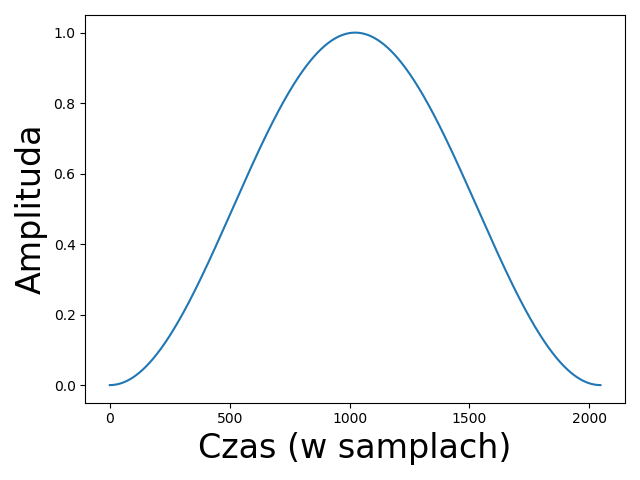
\includegraphics[width=.49\linewidth]{images/windowFunctions/HannWindow.png}
    \caption{Okno Hanna}
  \end{subfigure}
  \newline
  \begin{subfigure}{0.5\textwidth}
    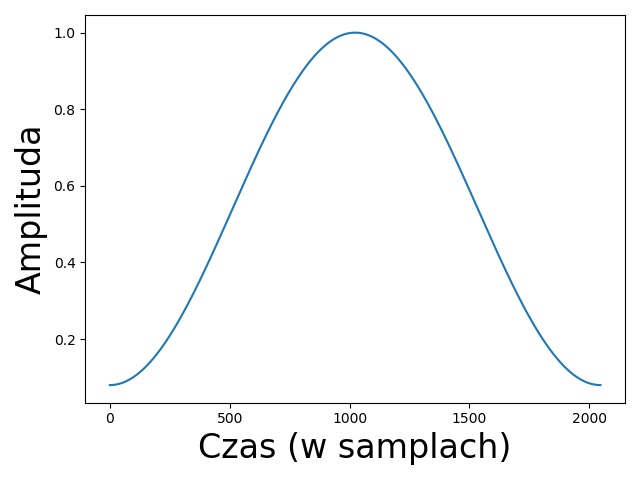
\includegraphics[width=1.\linewidth]{images/windowFunctions/HammingWindow.png}
    \caption{Okno Hamminga}
  \end{subfigure}
  \begin{subfigure}{0.49\textwidth}
    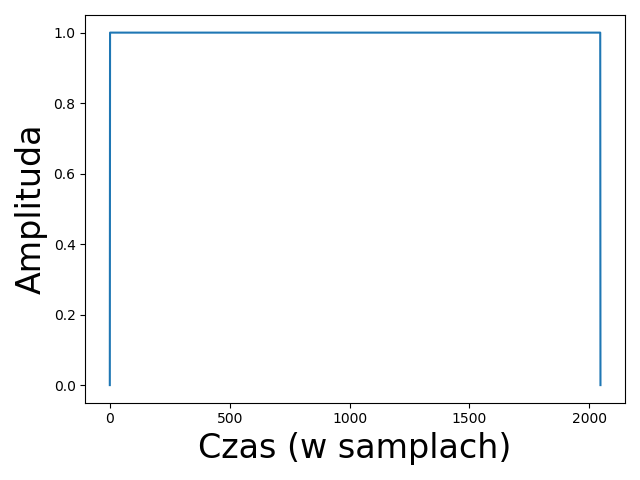
\includegraphics[width=1.\linewidth]{images/windowFunctions/RectangleWindow.png}
    \caption{Okno prostokątne}
  \end{subfigure}
  \caption{Przykład funkcji okna czasowego dla okna audio długości 2048 sampli.}
  \label{fig:WindowFunctions}
\end{figure}


W momencie, gdy w algorytmie okno nakłada się na siebie, pewna porcja danych jest duplikowana. Ilość redundantnych danych jest proporcjonalna do szerokości nakładania się na siebie okien. Aby zminimalizować ten negatywny efekt, na okno nakładana jest funkcja dalej zwana funkcją okna. W ogólności, funkcja okna wydobywa odpowiednio przemnożone wartości wewnątrz jej zakresu (w oknie) i stałą wartość (zazwyczaj jest to zero) wszędzie poza obrębem zakresu okna. Dla okien czasowych można stosować wiele różnych funkcji matematycznych. W tabeli ~\ref{tab:definicjeOkien} przedstawione są funkcje $w(t)$, które często wykorzystywane są jako okna czasowe w analizie sygnału akustycznego, wraz z ich analitycznymi wzorami widm $W(\omega)$. Graficzna reprezentację okna prostokątnego, Hanna oraz Hamminga można zobaczyć na rysunku \ref{fig:WindowFunctions}
\cite[87-90]{CyfrowePrzetwarzanieSygnalowOdTeoriiDoZastosowan}
%\cite[r. 4.4]{CyfrowePrzetwarzanieSygnalowOdTeoriiDoZastosowan}
\cite{Transcription:Kunieda:Aclos}.

\begin{table}[t]
  \begin{center}
    \begin{tabular}{ |c|c|c| } 
    \hline
    Nazwa funkcji & $w(t)$ & $W(\omega)$\\
    \hline
    Prostokątna & $p_T (t) = \left\{
      \begin{array}{ll}
        1 \text{ dla } |t| <= T\\
        0 \text{ dla } |t| > T\\
      \end{array}
    \right.  $ & $2\frac{\sin \omega T}{\omega}$\\
    \hline
    Trójkątne (Bartletta) & $q_T = \left\{
      \begin{array}{ll}
        1-|t|/T \text{ dla } |t| <= T\\
        0 \text{ dla } |t| > T\\
      \end{array}
    \right. $ & $T[\frac{\sin(\omega T / 2)}{\omega T/2}]^2$\\
    \hline
    Hanninga (Hanna) & $[0,5 + 0,5 \cos(\pi t / T)]p_T (t)$ & 
    $\frac{\pi^2 \sin(\omega T))}{\omega(\pi^2 - T^2 \omega^2)}$\\
    \hline
    Hamminga & $[0,54 + 0,46\cos(\pi t/T)]p_T (t)$ & 
    $\frac{(1,08\pi^2 - 0,16T^2\omega^2)}{\omega(\pi^2 - T^2 \omega^2))}\sin(\omega T)$\\
    \hline
    \end{tabular}
  \end{center}
  \caption{Definicje funkcji okien czasowych $w(t)$ i analityczne wzory ich widm $W(\omega)$}
  \label{tab:definicjeOkien}
\end{table}

\subsubsection{Przetwarzanie transformacji Fouriera}\label{sec:przetwarzanieFFT}
Wynikiem FFT jest wektor liczb zespolonych, którego długość jest równa długości danych (wielkości okna + długość wypełnienia zerami). Urojona część wyniku transformaty jest niezbędna do odwrócenia procesu transformacji, lecz nie jest niezbędna w procesie analizy. Większość algorytmów używających FFT przetwarza i skaluje wynik, aby pozbyć się niepotrzebnych informacji a istotne cechy uwypuklić. Powszechnie używaną techniką podczas analizy sygnałów jest operowanie na logarytmie amplitudy spektrum 
\cite[501-507]{Transcription:Talkin:RAPT}
%\cite[r. 2]{Transcription:Talkin:RAPT}
. Polega to na zastosowaniu normy Gaussa na każdej z wartości spektrum, co w rezultacie zniweluje część urojoną komponentu, a następnie zastosowanie na wyniku logarytmu naturalnego. Logarytm użyty jest do normalizacji i wyrównania danych przy zachowaniu relatywnych wartości. Wzór na logarytm amplitudy spektrum można przedstawić następująco:
\begin{equation}\label{eq:logPowSpec}
S_k^w(t,f) = ln||STFT_k^w(t,f)||
\end{equation}
gdzie $STFT_k$ jest $k$-tym komponentem spektrogramu. Częstą techniką jest również użycia potęgowania zamiast logarytmu, co zostało dokłądniej opisane w sekcji \ref{sec:f0:tfr}.
%%% chyba nie trzeba - \todo[inline]{Wykres STFT vs log(||STFT||)}

Przy analizie częstotliwości składowych widmowych sygnału na uwadzę należy mieć twierdzenie Nyquista, zwane także jako twierdzenie Kotielnikowa - Shannona lub \textit{twierdzeniem o próbkowaniu}. Mówi ono o istnieniu częstotliwości Nyquista, która opisana jest wzorem:
\begin{equation} \label{eq:NyquistFq}
  f_{Nyquist} = \frac{1}{2}v
\end{equation}
gdzie $v$ jest częstotliwością próbkowania. Częstotliwość ta jest maksymalną częstotliwością, jaką można wydobyć z sygnału o zadanej częstotliwości próbkowania. Odwracając proces, wzór \ref{eq:NyquistFq} mówi o tym, że częstotliwość próbkowania $v = \frac{1}{\delta t}$ musi być dobrana tak, aby była dwa razy większa od maksymalnej częstotliwości występującej w sygnale.

\begin{figure}[t]
  \begin{center}
    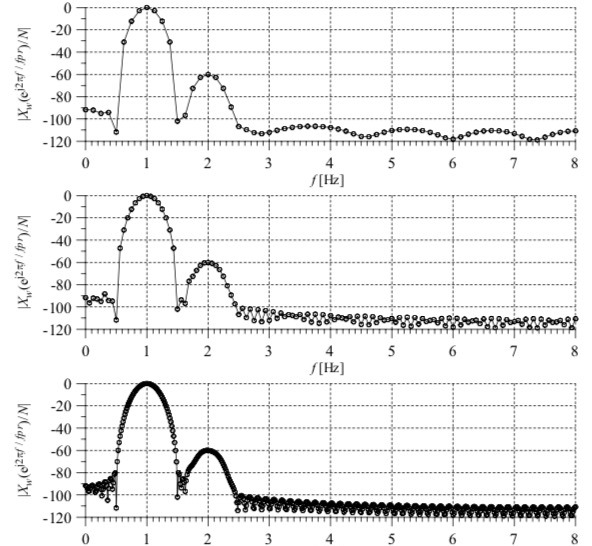
\includegraphics[scale=0.7]{images/ZeroPadding.jpg}
    \caption{Przykład analizy częstotliwościowej z wykorzystaniem STFT. Każdy z wykresów przedstawia to samo okno po uzupełnieniu na końcu zerami do długości $N_FFT$ = 128, 256, 1024 (kolejno od góry). Wykres z 
    \cite[224]{CyfrowePrzetwarzanieSygnalowOdTeoriiDoZastosowan}
    %\cite[r. 8.6]{CyfrowePrzetwarzanieSygnalowOdTeoriiDoZastosowan}
    }
    \label{fig:ZeroPadding}
  \end{center}
\end{figure}

Przy modelowaniu systemu transkrypcji często trzeba podjąć trudną decyzję, czy zwiększyć złożoność obliczeniową i osiągnąć lepszą aproksymację widma podczas FFT poprzez zwiększenie częstotliwości próbkowania lub zastosowanie interpolacji, czy zmniejszyć dokładność, ale otrzymać mniejszą złożoność obliczeniową. Istnieje jednak metoda, która prowadzi do kompromisu tych dwóch podejść. Polega ona na uzupełnieniu na końcu zerami analizowanego, fragmentu sygnału tuż po nałożeniu funkcji okna. Po tak wykonanej konkatenacji danych można zastosować STFT. Podejście to daje w wyniku gęściejsze próbkowanie widma przy mniejszych nakładach obliczeniowych. Tak zwiększoną rozdzielczość widma można zaobserwować na rysunku \ref{fig:ZeroPadding} 
\cite[221-224]{CyfrowePrzetwarzanieSygnalowOdTeoriiDoZastosowan}
%\cite[r. 8.6]{CyfrowePrzetwarzanieSygnalowOdTeoriiDoZastosowan}
.

\clearpage

\section{Estymacja częstotliwości fundamentalnej w sygnale monofonicznym}\label{sec:f0}
Ten rozdział skupia się na opisaniu metod estymacji składowej fundamentalnej w sygnale akustycznym. Jest to jeden z kroków wymaganych do pełnej transkrypcji utworu muzycznego, a przez wielu badających ten teren nauki uważany za najważniejszy 
\cite[408-415]{Transcription:Klapuri:ChallengesAndFuture}
%\cite[r. 1-2]{Transcription:Klapuri:ChallengesAndFuture}
. Wysokość dźwięku jest niezwykle istotną informacją z punktu widzenia muzyka, a sposób zagrania poszczególnych nut determinowany jest właśnie przez F0. Nawiązując do informacji opisanych w rozdziale \ref{sec:JakDzialaMuzyka} aby poprawnie wykryć F0 należy przeanalizować wiele czynników. 

Samo rozpoznanie wysokości tonu jest kategoryzowane w zależności od specyfiki sygnału wejściowego na transkrypcję utworów monofonicznych (dla sygnału bez równoległych dźwięków) oraz transkrypcję utworów polifonicznych (dla sygnałów z równoległymi dźwiękami). Te drugie są często dalej dzielone na transkrypcję sygnałów mono- i multiinstrumentalnych (w zależności od tego, czy w sygnale występuje tylko jeden lub więcej instrumentów o różnych barwach dźwięku).

Dalsze rozważania będą przebiegać z założeniem, że przetwarzane sygnały są z podzbioru muzyki o standardach kompozycji zachodniej, lecz bez wyszczególnionego gatunku muzycznego. Nie będziemy również skupiali się na wykryciu tak zwanych dźwięków o niezależnej wysokości, do których zaliczają się elementy perkusyjne. Ważnym założeniem, które jest stosowane w tym rozdziale, jest analiza jedynie sygnałów monofonicznych. W odróżnieniu do krzywych reprezentujących muzykę polifoniczną, w analizowanych utworach będzie grany tylko jeden dźwięk na pojedyńczym instrumencie, bez równoległych dźwięków. Algorytmy analizujące muzykę wielotonową są opisane w rozdziale \ref{sec:MultiPitch}. Jest to bardzo duże ułatwienie, ponieważ konkurujące sygnały dźwiękowe nakładają się na siebie, zmuszając algorytm analizujący do rozróżnienia i odseparowania ich przed faktyczną analizą F0. 

\subsection{Funkcja autokorelacji}\label{sec:f0:ac}
Domena czasu jest najbardziej naturalną postacią sygnału dźwiękowego, ponieważ w takiej właśnie postaci jest odbierane przez ludzkie ucho - jako ciśnienie akustyczne zmienne w czasie. Wiele z pierwszych badań jakie prowadzono w kontekście transkrypcji sygnału fonicznego wykorzystywało tą postać sygnału, między innymi w przytoczonej wcześniej pracy \cite{Transcription:Gold:ComputerProgramForPitchExtraction}. Algorytm ten polegał na znajdywaniu wzorców w krzywej sygnału. Regularności, które powtarzały się okresowo co $T$, były analizowane jako kandydaci F0. Jak analiza czystego binarnego sygnału i wyliczenia na nim nie są częstą praktyką, tak podejście do znajdywania wzorców i regularności jest powszechna we współczesnych algorytmach. Najbardziej dosłowne odwzorowanie tej idei można znaleźć w metodologiach opartych na korelacji, której celem jest znalezienie wysokości dźwięku 
\cite[41-44]{Transcription:Quenneville:Thesis}
%\cite[r. 5.2]{Transcription:Quenneville:Thesis}
.

\textit{Autokorelacja} jest narzędziem matematycznym stosowanym w przetwarzaniu sygnałów. Służy ono do analizy serii wartości. Ta statystyczna miara odwzorowuje podobieństwo pomiędzy kolejnymi wartościami tej samej zmiennej. Funkcja ta ma za zadanie wykrycie regularności w analizowanych danych 
\cite[14-17]{CyfrowePrzetwarzanieSygnalowOdTeoriiDoZastosowan}
%\cite[r. 1.3.5]{CyfrowePrzetwarzanieSygnalowOdTeoriiDoZastosowan}
. Proces autokorelacji polega na badaniu korelacji wejściowych danych z tymi samymi danymi, ale przesuniętymi o pewną wartość (przesunięcie, z ang. \textit{lag}). Siła korelacji o odpowiednim przesunięciu może świadczyć o powtarzającym się wzorze w sygnale z częstotliwością przesunięcia.

W pracy naukowej \cite{Transcription:Lawrence:AutocorrelationForPitchDetection} Lawrence używa funkcji autokorelacji do wykrycia częstotliwości fundamentalnych w zadanym sygnale monofonicznym. Zakłada on, że badany sygnał jest quasi-periodyczny, co oznacza, że sygnał posiada cechy pojawiające się w prawie równych odstępach, lecz nie musi być on bezbłędnie periodyczny. Sygnał w pełni periodyczny jest przedmiotem analizy czysto teoretycznej, ponieważ sygnał akustyczny musiałby pozostać bez zmian w amplitudzie i częstotliwości przez cały swój okres, podczas gdy sygnał quasi-periodyczny zakłada zmiany w strukturze sygnału względem czasu. Funkcja autokorelacji na takim sygnale byłaby funkcją długości okresu opisującą zgodność przesuniętego o ten okres sygnału z sygnałem bazowym. 

Wzór na ogólną postać funkcji autokorelacji od długości okresu $h(t)$ jako:
\begin{equation}\label{eq:AC}
  R(k) = \lim_{N \to \infty} \frac{1}{2N + 1} \sum_{n=-N}^{N} h(n)h(n + k)
\end{equation}
gdzie $k$ jest opóźnieniem, $n$ reprezentuje moment w czasie a N reprezentuje długość badanej funkcji. Jak można zaobserwować w \ref{eq:AC} założeniem jest, że sygnał bazowy jest nieskończenie długi (tak samo jak przy TF opisanej w sekcji \ref{sec:TF}). Do rozważań w kontekście analizy sygnału fonicznego będziemy używać wariancji krótkoczasowej tego wzoru, operującej na oknach danych (analogicznie do STFT opisanej w sekcji \ref{sec:STFT}) opisanej w 
\cite[503]{Transcription:Talkin:RAPT}
%\cite[r. 2.2.2]{Transcription:Talkin:RAPT}
 jako:
\begin{equation}\label{eq:STAC}
  R(i,k) = \sum_{j=m}^{m + N - k - 1} h_jh_{j+k}, m = iz
\end{equation}
gdzie $i$ jest indeksem badanego okna, $z$ jest odstępem pomiędzy oknami audio (ilość sampli), a N jest długością okna. Zgodnie z twierdzeniem Nyquista opisanym w sekcji \ref{sec:STFT} długość okna powinna być co najmniej dwa razy większa niż największe oczekiwane opóźnienie jakie może wystąpić w analizowanym sygnale akustycznym. Implementacja estymacji F0 przy pomocy autokorelacji została opisana w sekcji \ref{sec:impl:alg:ac}.

Z jednego okna danych w wyniku wyznaczane jest to przesunięcie, które ma największy współczynnik korelacji. Dlatego, że domena czasu w dyskretnym sygnale na jakiej operuje autokorelacja jest tak naprawdę domeną ilości sampli, aby uzyskać wynik w postaci częstotliwości należy podzielić częstotliwość samplowania przez wyznaczone przesunięcie:
\begin{equation}\label{eq:AC:hz}
  fq = \Delta/lag
\end{equation}

\begin{figure}[t]
  \begin{subfigure}{.5\textwidth}
    \centering
    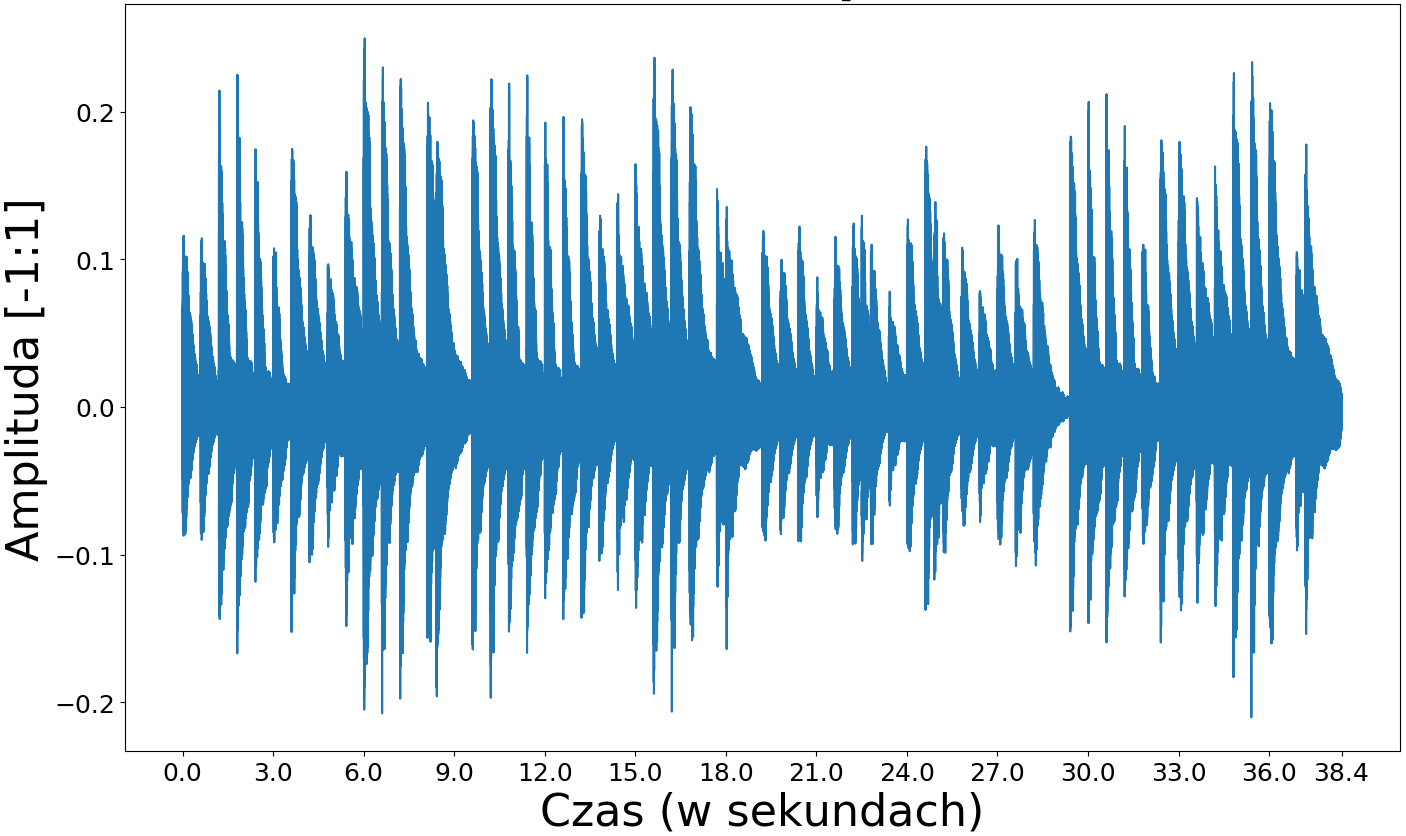
\includegraphics[width=1.\linewidth]{images/AC/fala_cropped.png}
    \caption{Fala dźwiękowa}
    \label{fig:ACResults:wave}
  \end{subfigure}%
  \begin{subfigure}{.5\textwidth}
    \centering
    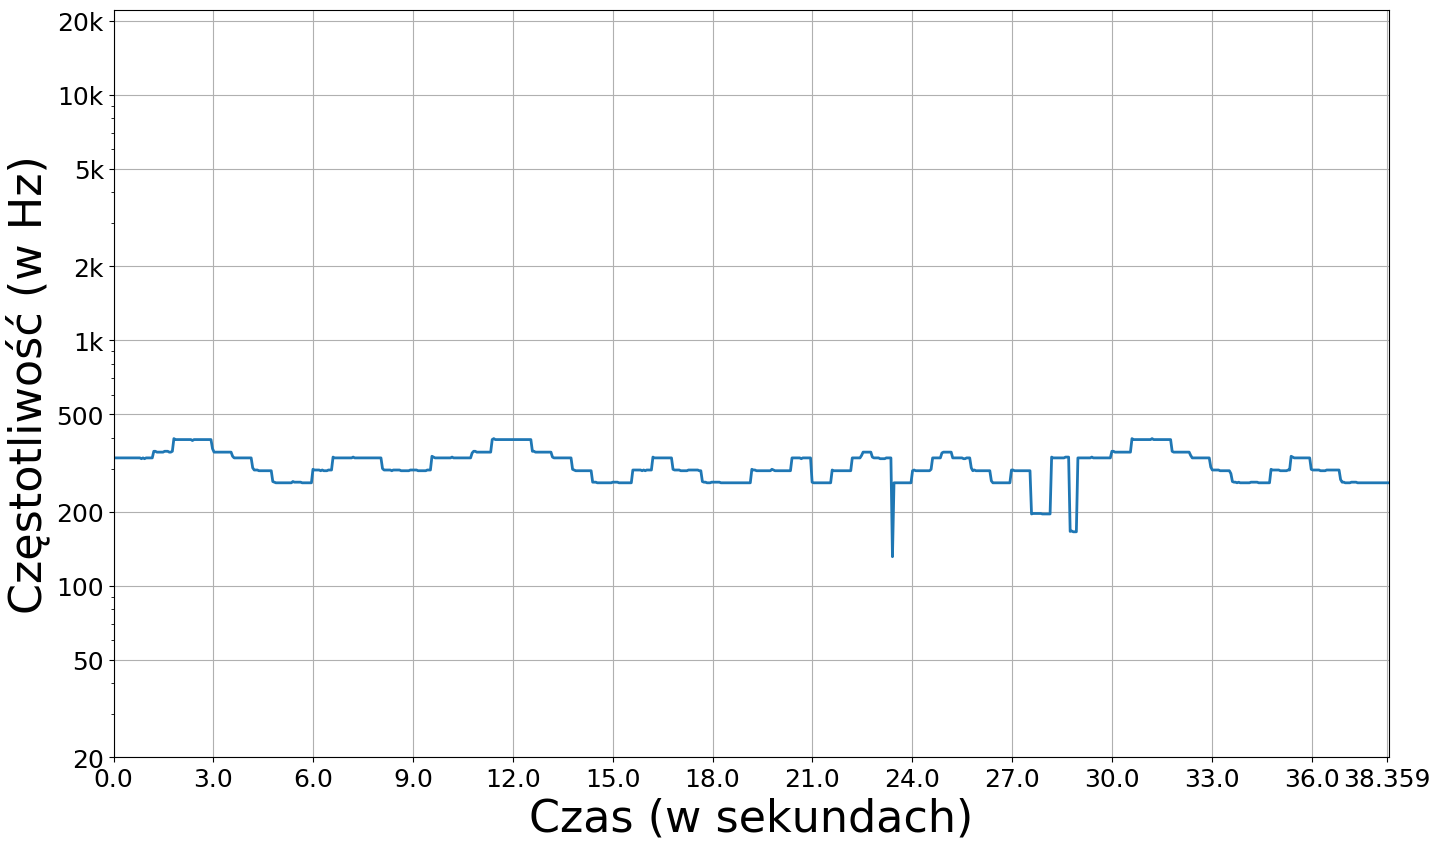
\includegraphics[width=1.\linewidth]{images/AC/f0Thick_cropped.png}
    \caption{Estymacja F0}
    \label{fig:ACResults:f0}
  \end{subfigure}
  \newline
  \begin{subfigure}{1\textwidth}
    \centering
    % include third image
    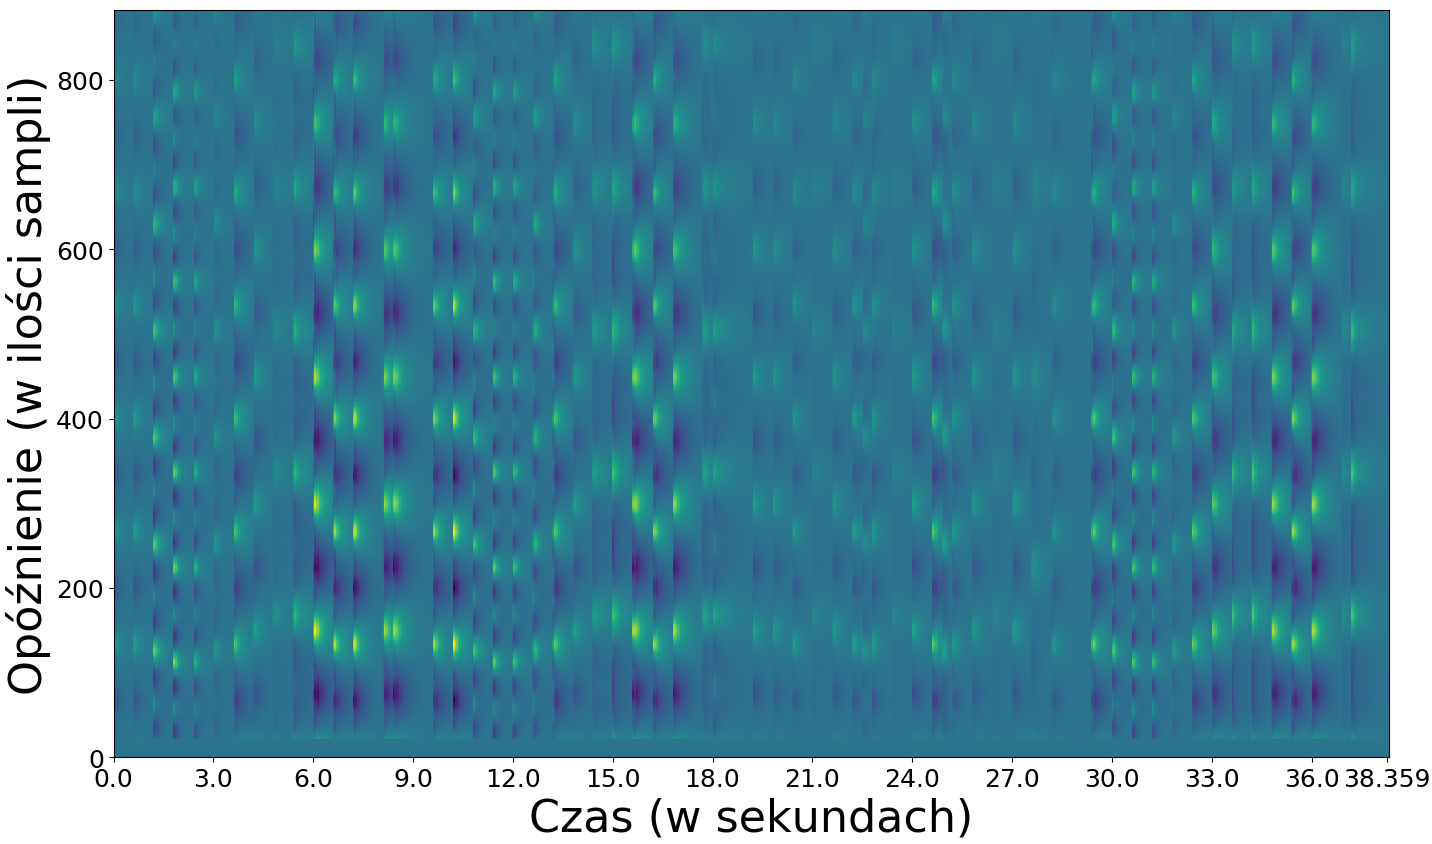
\includegraphics[width=.6\linewidth]{images/AC/korelogram_cropped.png}  
    \caption{Korelogram}
    \label{fig:ACResults:corr}
  \end{subfigure}
  \caption{Wynik autokorelacji na kompozycji ,,Oda do radości'' IX symfonii Beethovena zagranej monofonicznie na pianinie. Użyto okno Hanna o długości 2048 sampli z odstępami długości 2048 sampli. Wybór F0 polegał na wybraniu największego współczynnika korelacji w oknie. Jaśniejsze obszary na korelogramie oznaczają większą magnitudę.}
  \label{fig:ACResults}
\end{figure}

Podstawowym założeniem algorytmów wykrywania F0 z wykorzystaniem autokorelacji (tak samo jak znormalizowanej korelacji krzyżowej, która stara się zminimalizować defekty funkcji autokorelacji, dokładny jej opis można znaleźć w pracy \cite{Transcription:Talkin:RAPT}) jest to, że analizowany sygnał jest monofoniczny. Jest to spowodowane tym, że periodyczność jaką cechuje się pojedyńcza krzywa quasi-periodyczna jest modulowana, albo nawet całkowicie neutralizowana po nałożeniu na nią innej krzywej. Załóżmy, że został nagrany sygnał z dwoma nutami o różnych wysokościach granymi równolegle w tym samym czasie. Okresami, w którym te sygnały w izolacji byłyby powtarzalne to $T_1$ i $T_2$. Po nałożeniu się na siebie, wynikowy sygnał nie byłby periodyczny w żadnym z tych interwałów, chyba że jeden byłby wielokrotnością drugiego Jest to opisane dokładniej w sekcji \ref{sec:MultiPitch:monofon}.

Wyniki estymacji F0 mają tendencje do bycia wielokrotnościami faktycznego F0 sygnału, co można zaobserwować na wykresach na wykresie \ref{fig:ACResults:f0}. Dzieje się tak, ponieważ wysoki współczynnik korelacji, jaki uzyska krzywa o periodyczności równej $T$ dla opóźnienia $T$ będzie relatywnie podobny do wyniku autokorelacji dla tego sygnału dla opóźnienia $2T$, $3T$ itd. Jest to spowodowane tym, że wzorzec występujący co $T$ występuje w szczególności co $2T$, $3T$ itd. Można to również zaobserwować w korelogramie przedstawionym na rysunku \ref{fig:ACResults:corr} 
\cite[231-244]{Transcription:Anssi:SignalProcessingMethods}
%\cite[8.2.1-8.3.3]{Transcription:Anssi:SignalProcessingMethods}
.

\subsection{Analiza TFR} \label{sec:f0:tfr}
Analiza sygnału w reprezentacji średniego poziomu TFR, w przeciwieństwie do operowania na nieprzetworzonym sygnale cyfrowym, jak miało to miejsce w sekcji \ref{sec:f0:ac}, skupia się na badaniu relacji w domenie częstotliwości danego sygnału. Najpopularniejszą reprezentacja TRF jest zdefiniowana jako STFT na kolejnych fragmentach (oknach) sygnału. Docelową postacią jest zbiór okien tworzących spektrogram, ale w celu jego uzyskania należy SFTF przedstawić jako wektor energii. Jednym ze sposobów w jaki można uzyskać taką postać jest to wykonanie kwadratu modułu z STFT:

\begin{equation} \label{eq:powSpec}
  SP_x^w(t,f) = |STFT_x^w(t,f)|^2
\end{equation} 
Wynik powyższego równania \ref{eq:powSpec} nazywany jest potocznie widmem mocy (z ang. \textit{power spectrum}). W celu uzyskania spektrogramu używa się również innych metod, jak na przykład logarytmu z modułu (co zostało to opisane w sekcji \ref{sec:przetwarzanieFFT}). Wybór metodyki zależny jest od tego, które cechy sygnału wejściowego są bardziej, a które mniej istotne w kontekście algorytmu analizującego. Użycie widma mocy wiąże się z uwydatnieniem już wyraźnych cech, wraz z zwiększeniem istotności szumu w sygnale.

\begin{figure}[t]
  \begin{subfigure}{.49\textwidth}
    \centering
    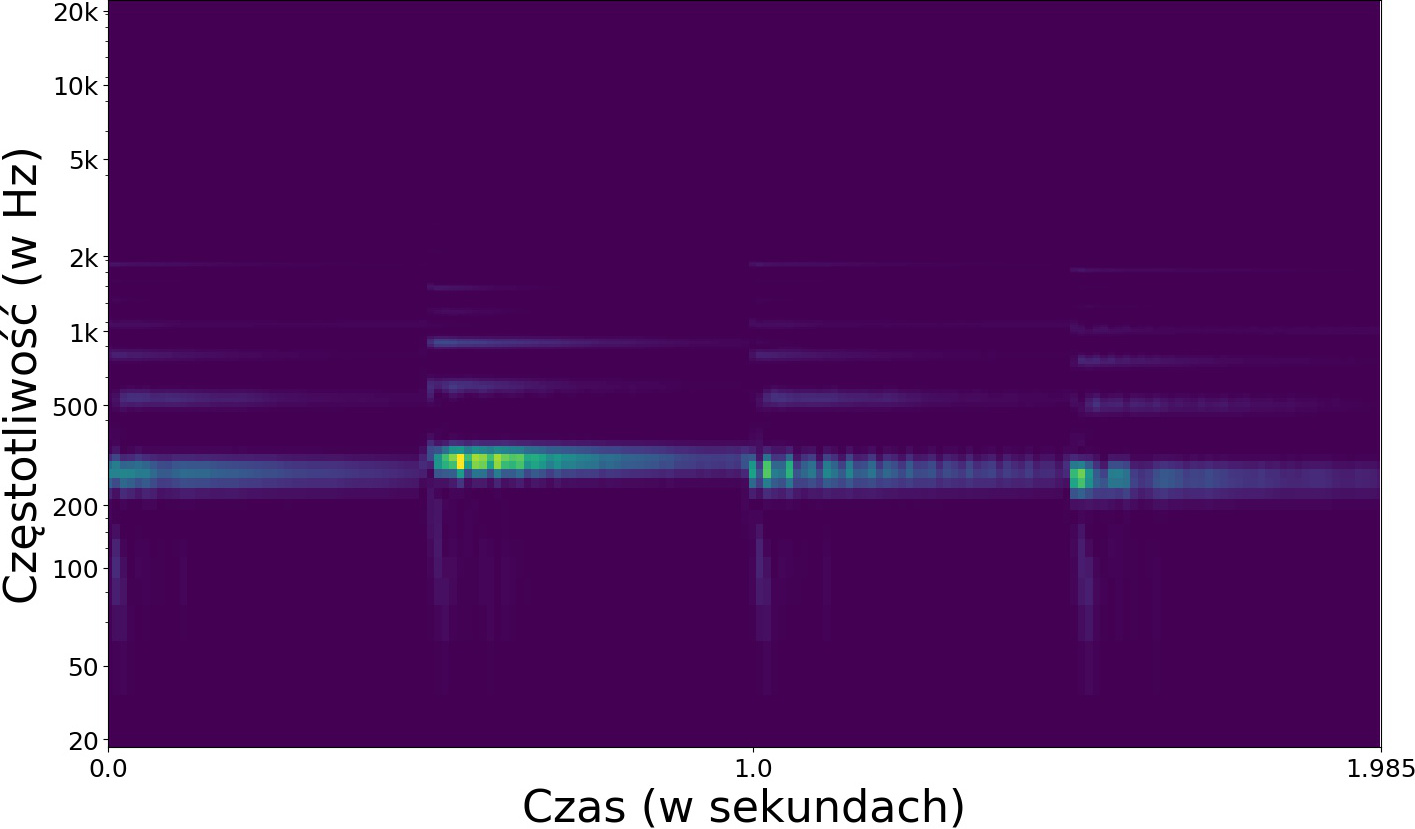
\includegraphics[width=1.\linewidth]{images/Spectrogram/spectrogram_1024_cropped.jpg}
    \caption{Spektrogram z długością okna 1024 sample}
  \end{subfigure}
  \begin{subfigure}{.5\textwidth}
    \centering
    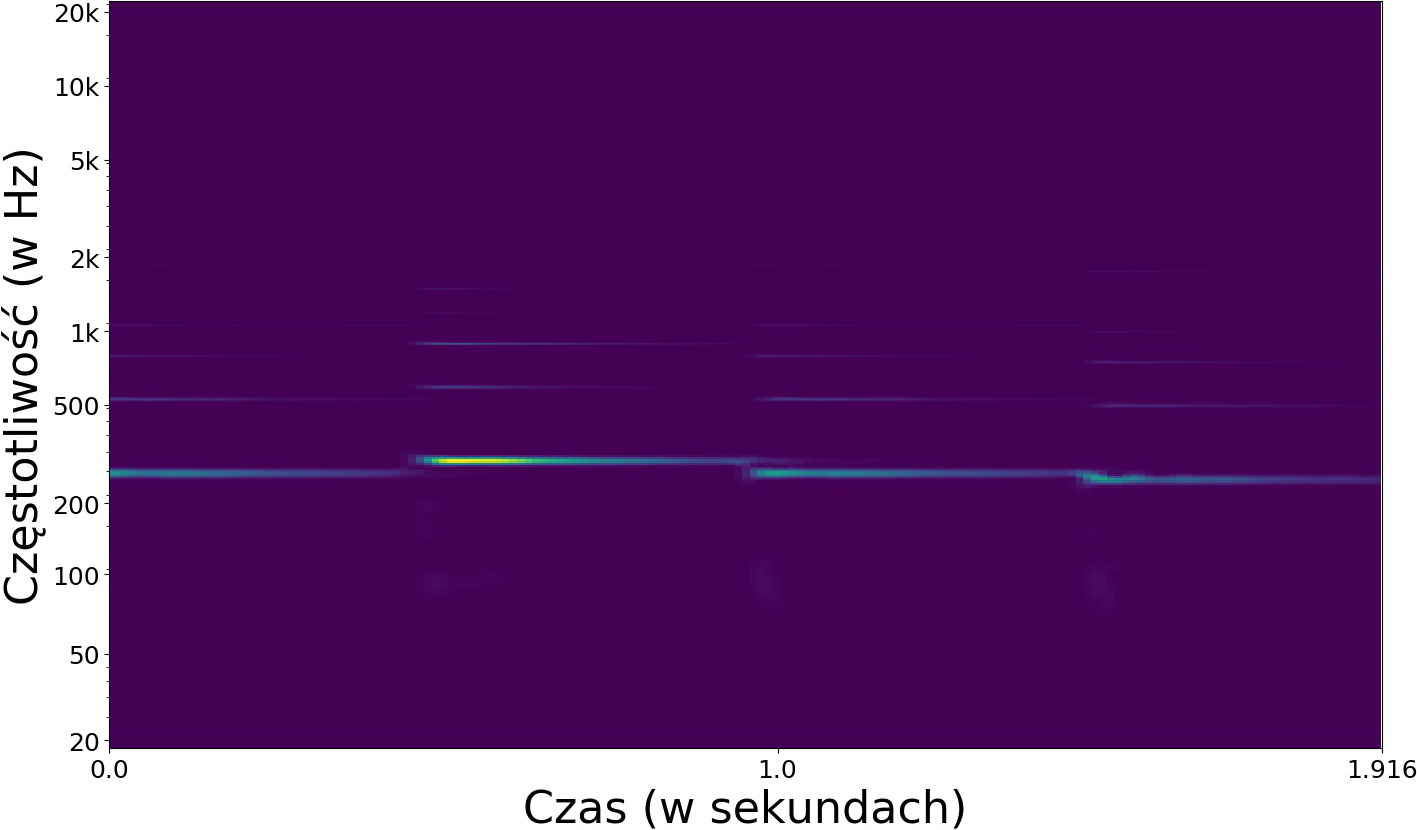
\includegraphics[width=1.\linewidth]{images/Spectrogram/spectrogram_4096_cropped.jpg}
    \caption{Spektrogram z długością okna 4096 sample}
  \end{subfigure}
  \caption{Spektrogramy sygnału sekwencji C3-D3-C3-B2 zagranej na pianinie wyliczone przy pomocy STFT z oknem Hanna długości odpowiednio 1024 i 4096 dla wykresów (a) i (b) z odstępami o długości 512 sampli. Jaśniejsze obszary oznaczają większą magnitudę.}
  \label{fig:windowSize}
\end{figure}

Zmiana funkcji okna $w$ zmieni specyfikę STFT, co przekłada się na inny wynikowy spektrogram. Długość użytego okna jest także istotną cechą spektrogramu. Zmiany w dokładności poszczególnych wartości spektrogramu przy różnych długościach okna opisane są w sekcji \ref{sec:STFT} i widoczne na ilustracji \ref{fig:windowSize}.

Podczas analizy spektrogramu, naiwnym podejściem byłoby wybranie za F0 ten pik w spektrum, który ma największą energię. Niestety jednak nie jest to zawsze prawidłowy wybór - częstotliwość fundamentalna wcale nie musi być tą, która ma najwięcej energii w sygnale akustycznym. Ze względu na charakterystyki różnych instrumentów, formanty, szum i inne zniekształcenia opisane dokłądniej w sekcji \ref{sec:barwaDzwieku} kolejne harmoniczne mogą być wzmocnione ponad F0.

\begin{figure}[t]
  \begin{center}
    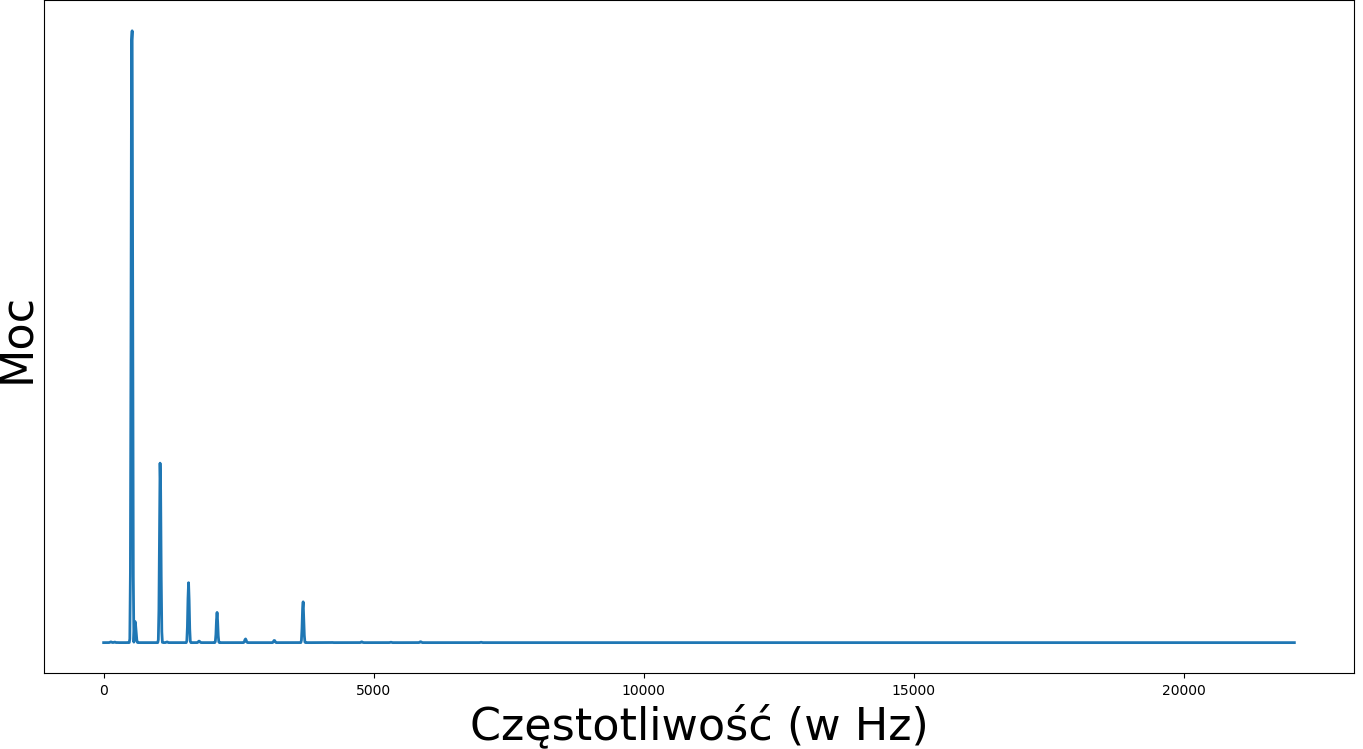
\includegraphics[scale=0.26]{images/Spectrogram/spectrum_4096_cropped.jpg}
    \caption{Przykład pojedyńczego komponentu spektralnego ze spektrogramu \ref{fig:windowSize} o długości okna 4096.}
    \label{fig:spectralComponent}
  \end{center}
\end{figure}

Analiza spektrogramu w celu znalezienia F0 polega na znalezieniu korelacji w rozmieszczeniu harmonicznych względem siebie. Zgodnie z regułą harmoniczności, harmoniczne sygnału mają częstotliwości będące wielokrotnościami fundamentalnej częstotliwości. Są one równomiernie rozmieszczone na przestrzeni całego spektrum, co powoduje, że pojedyńcza nuta jest sama w sobie periodyczna w domenie częstotliwości, co można zauważyć na rysunku \ref{fig:spectralComponent}. Ta charakterystyka jest powszechnie używana w wykrywaniu częstotliwości fundamentalnej sygnału akustycznego.

\subsection{Analiza cepstralna}\label{sec:f0:ceps}
Z racji tego, że spektrum samo w sobie jest periodyczne, możliwe jest użycie metodologi wykrywającej cykliczności na spektrum. Taki pomysł mieli już w 1963 Bogert, Healy i Tukey w \cite{Transcription:Bogert:FirstCepstrum}. Wynaleźli oni narzędzie matematyczne przeznaczone dla danych zawierających echa lub pogłosy fundamentalnej częstotliwości, która nie jest znana. \textit{Cepstrum mocy} używane jest do wyznaczenia czasu początku danego dźwięku, jego echa i powiązanych amplitud. Analiza na zespolonym cepstrum pozwala na powrót do pierwotnego kształtu badanego \cite{Transcription:Childers:CepstruGuide} 
\cite[46-50]{Transcription:Quenneville:Thesis}
%\cite[r. 5.3, r. 5.3.1]{Transcription:Quenneville:Thesis}
.

W roku 1967 cepstrum zostało zastosowane do wykrywania wysokości dźwięku w ramach pracy \cite{Transcription:Noll:CepstrumPitchDetermination}. Jak opisuje Oppenheim i Schafer w pracy naukowej 
\cite[95-99]{Transcription:Oppenheim:HistoryOfCepstrum}
%\cite{Transcription:Oppenheim:HistoryOfCepstrum}
, która dotyczy historii tego narzędzia, równolegle i niezależnie z tymi badaniami powstawała praca doktorancka \cite{Transcription:Oppenheim:Superposition} badająca klasę nielinearnych technik przetwarzania sygnałów poprzez koncepcje homomorficznego mapowania pomiędzy grupami algebraicznymi i przestrzeniami wektorowymi. Ma ona szczególne zastosowanie w metodologii cepstralnej, pokrywając się wnioskami i przyspieszając tempo jego rozwoju. Dalsze prace Oppenheima opisujące między innymi charakterystyki splotu harmonicznych, które są bardzo podobne do spektrum logarytmu spektrum. Odkrycia te przyczyniły się do, między innymi, stosowania cepstrum na oknach czasowych (tak jak STFT) czy opisanie zespolonego cepstrum, które pozwala na odwrócenie tej transformacji, otwierając drogę do takich metod jak filtrowanie w domenie cepstralnej.

Oryginalnie analiza cepstralna, która została opisana w przytoczonej powyżej pracy \cite{Transcription:Bogert:FirstCepstrum} została zdefiniowana jako ,,spektrum mocy z logarytmu spektrum mocy''. Nawiązując do wzoru \ref{eq:logPowSpec}, cepstrum mocy okna o indeksie $k$ z oknem $w$ liczy się jako 
\begin{equation}\label{eq:ceps1}
  C_k^w(t, f) = |(S_k^w(t,f)|^2.
\end{equation}
Pierwotnym zastosowaniem tego narzędzia było wykrycie echa w sygnale sejsmicznym. Podejście to było bardziej odporne na barwę sygnału od wcześniej używanej funkcji autokorelacji (opisanej w sekcji \ref{sec:f0:ac}). Zastosowanie to było czysto analityczne, i nie wymagało od algorytmu możliwości przywrócenia analizowanych danych do domeny czasu. Mimo, że jednym z autorów pierwotnej pracy o cepstrum jest Tukey, który także pracował nad FFT, cepstrum zostało opublikowane na dwa lata przed pracą opisującą algorytm FFT \cite{Transcription:Tukey:FFT}, przez co jego potencjał nie był jeszcze odkryty. Choć w pierwotnej pracy nad cepstrum zdefiniowane były takie pojęcie jak ,,lifter'', był zainicjalizowany później z użyciem filtru konwolucyjnego 
\cite[1-2]{Transcription:Randall:CepstrumHistory}
%\cite[r. 1]{Transcription:Randall:CepstrumHistory}
.

Nazwa cepstrum bierze się z odwrócenia pierwszych liter wyrazu \textit{spectrum} (z ang. spektrum). Szereg terminologii został opisany na potrzeby zdefiniowania narzędzia cepstrum w pierwotnej pracy \cite{Transcription:Bogert:FirstCepstrum}, które do dziś są używane w celu wyróżnienia domen cepstralnych:
\begin{table}[H]\centering
  \begin{tabular}{lll}
  \textit{rahmonics} & zamiast & \textit{harmonics} (z ang. harmoniczność) \\
  \textit{liftering} & zamiast & \textit{filtering} (z ang. filtrowanie) \\
  \textit{quefrency} & zamiast & \textit{frequency} (z ang. częstotliwość) \\
  \textit{gamnitude} & zamiast & \textit{magnitude} (z ang. wielkość)
  \end{tabular}
\end{table}
\noindent Wytłumaczeniem tej lingwistyki, w której znajome wyrazy były modyfikowane w celu uzyskania czegoś podobnego, ale mimo wszystko troche innego, było zadeklarowane następująco: 
\begin{displayquote}
,,Ogólnie rzecz biorąc, działamy po stronie częstotliwości w sposób powszechnie stosowany po stronie czasu i odwrotnie'' 
\cite[95]{Transcription:Oppenheim:HistoryOfCepstrum} 
%\cite{Transcription:Oppenheim:HistoryOfCepstrum} 
(tłumaczenie własne)
\end{displayquote}

Cepstrum posiada piki tam, gdzie oryginalny sygnał w przestrzeni czasu - amplitudy posiada echo. Ta nowa reprezentacja spektralnej domeny nie jest już domeną częstotliwości, ani też nie jest to domena czasu. Przez ten fakt, aby nie mylić tych pojęć z pozostałymi Bogert nazwał domenę cepstrum jako domena \textit{quefrency}, która tak naprawdę jest domeną częstotliwości spektralnych pików oryginalnego sygnału 
\cite[1-4]{Transcription:Randall:CepstrumHistory}
%\cite[r. 1-2]{Transcription:Randall:CepstrumHistory}
.

W przypadku lifterowania, czyli filtrowania w domenie quefrency, używany jest wzór cepstrum sygnału ciągłego $x(t)$:
\begin{equation}\label{eq:ceps:continous}
Cep_x(\tau) \ ICFT_{log(|X|)}(\tau) = \int_{-\infty}^{\infty}  log(|X(f)|)e^{j2\pi f\tau}\,\mathrm{d}f, 
\end{equation}
gdzie  $X(f)$ oznacza TF. Zgodnie z tym wzorem filtrowanie sygnału w domenie częstotliwości przez wynik $X(f)H(F)$ staje się, po wzięciu $log$, sumą $log[X(f)] + log[H(f)]$ gdzie $H(f)$ jest filtrem częstotliwościowym 
\cite[25-27]{Transcription:Anssi:SignalProcessingMethods}
%\cite[r. 2.1.3]{Transcription:Anssi:SignalProcessingMethods}
.

\begin{figure}[t]
  \begin{subfigure}{.49\textwidth}
    \centering
    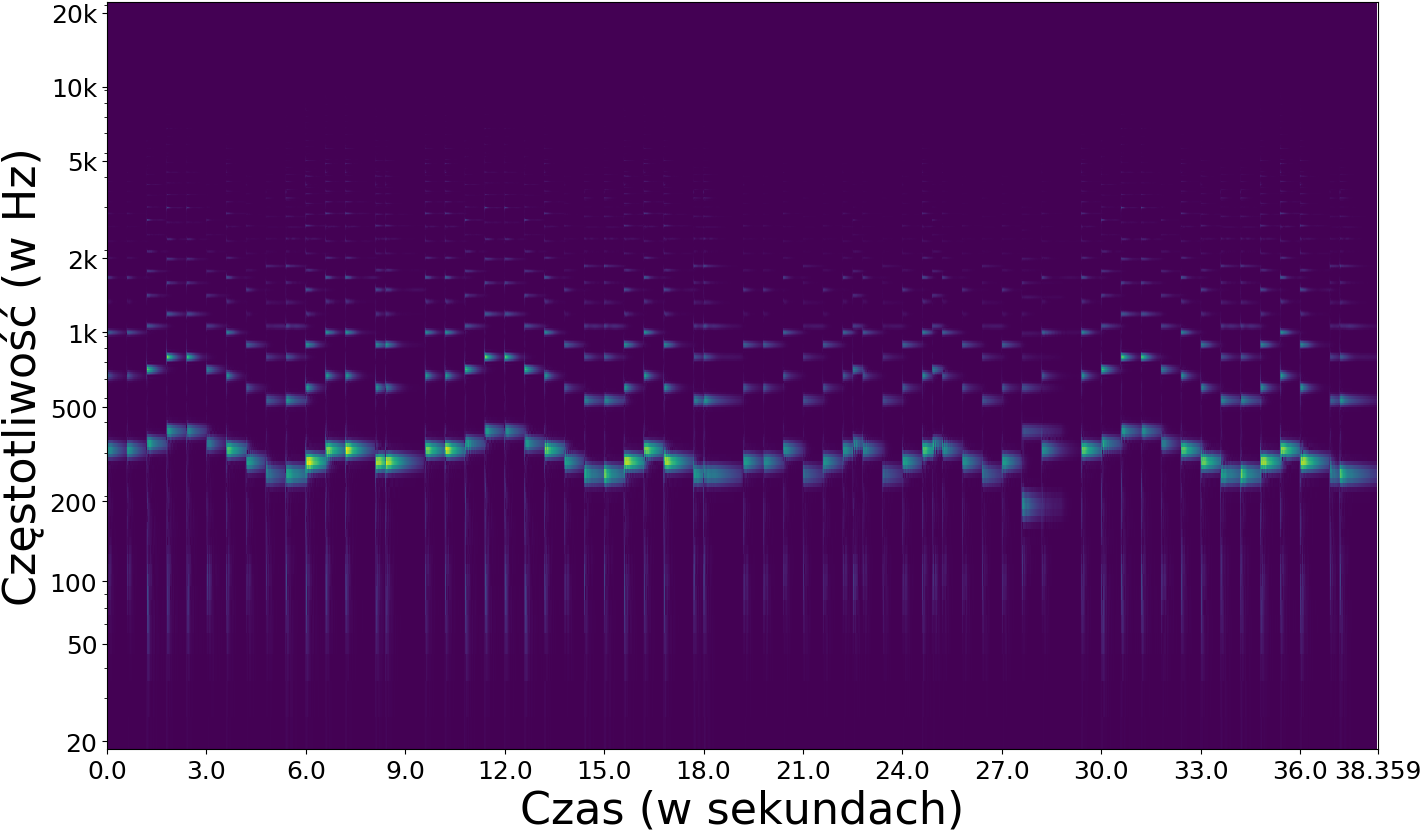
\includegraphics[width=1.\linewidth]{images/Cepstrum/spec_cropped.png}
    \caption{Spektrogram}
  \end{subfigure}
  \begin{subfigure}{.5\textwidth}
    \centering
    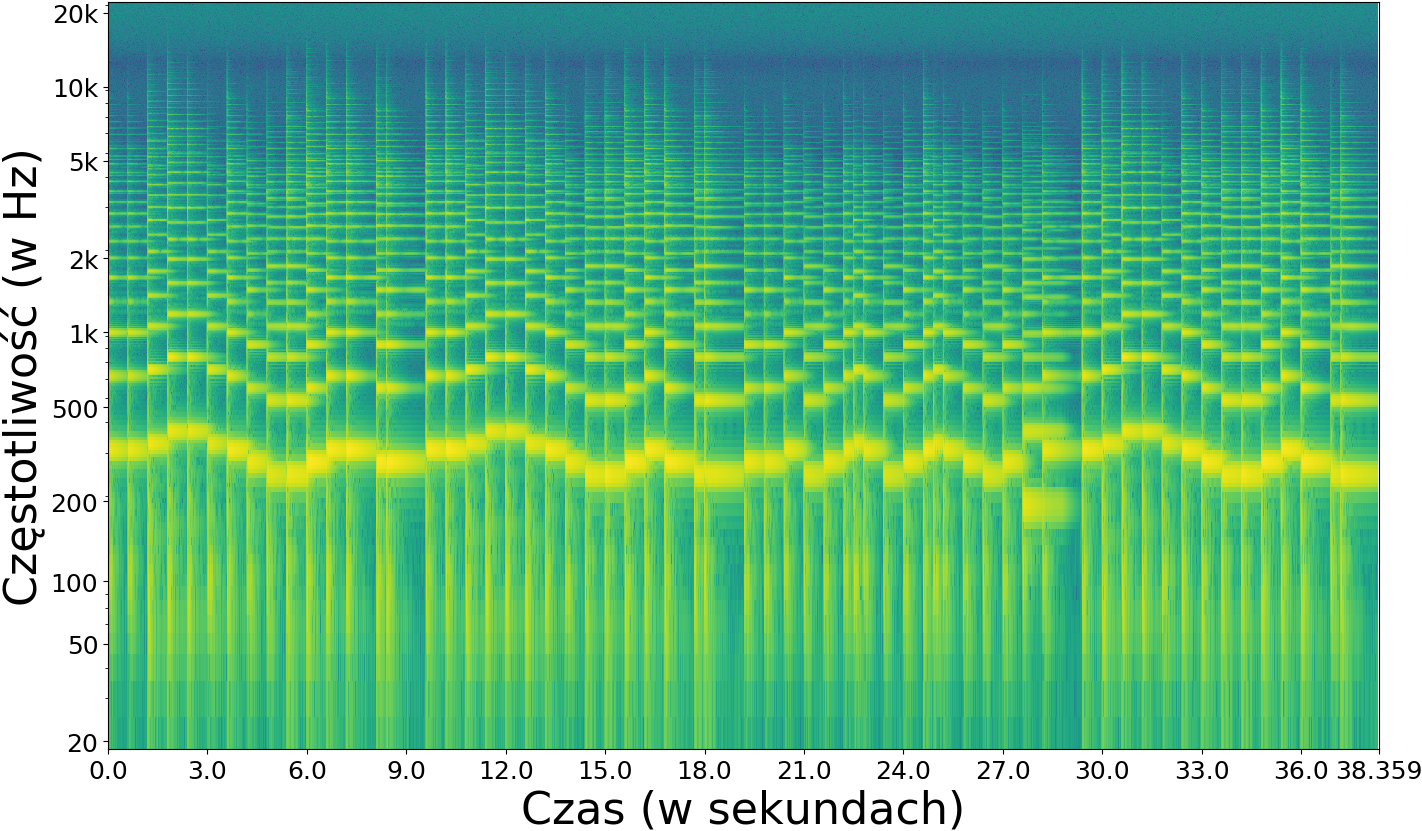
\includegraphics[width=1.\linewidth]{images/Cepstrum/log_pow_spec_cropped.png}
    \caption{Logarytm spektrogramu mocy}
  \end{subfigure}
  \newline
  \begin{subfigure}{.49\textwidth}
    \centering
    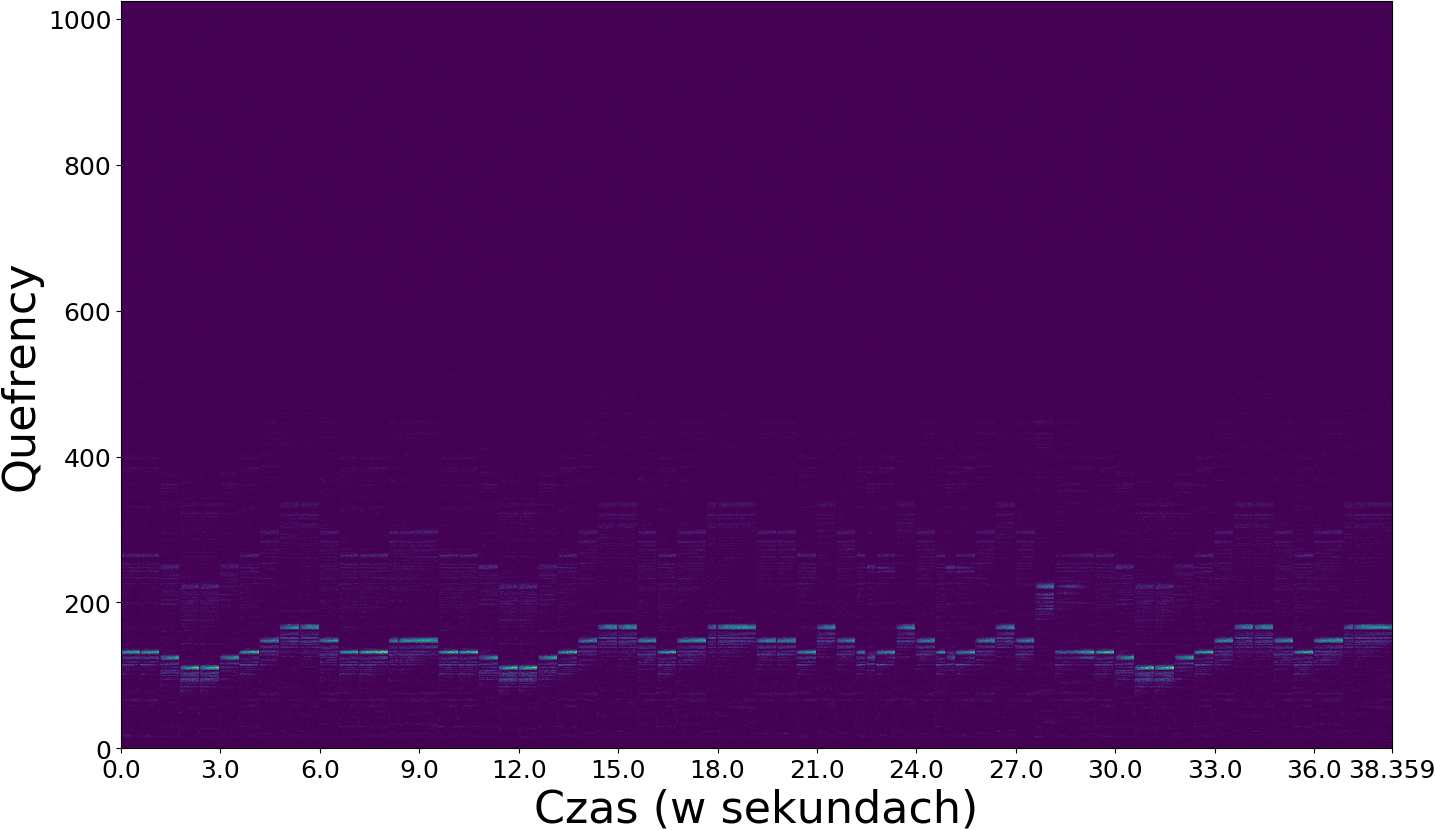
\includegraphics[width=1.\linewidth]{images/Cepstrum/cepstrogram_cropped.png}
    \caption{Cepstrogram}
  \end{subfigure}
  \begin{subfigure}{.5\textwidth}
    \centering
    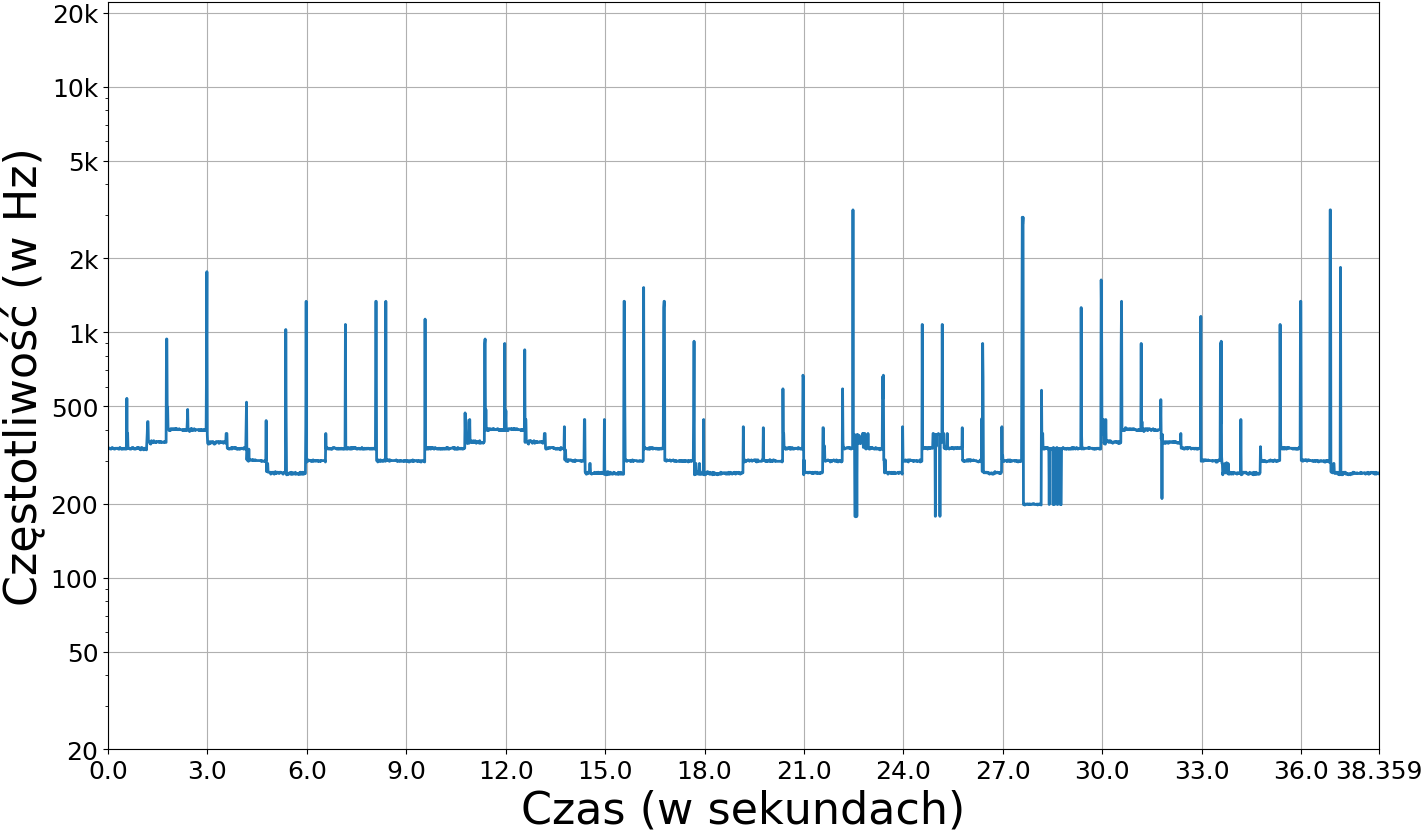
\includegraphics[width=1.\linewidth]{images/Cepstrum/estymacjaF0_cropped.png}
    \caption{Estymacja F0}
  \end{subfigure}
  \caption{Wynik cepstrum na na ,,Odzie do radości'' IX symfonii Beethovena zagranej monofonicznie na pianinie. Użyto okno Hanna o długości 2048 sampli z odstępami długości 512 sampli. Wybór F0 polegał na wybraniu największego współczynnika cepstralnego w oknie. Jaśniejsze obszary w spektrogramach i cepstrogramie oznaczają większą magnitudę.}
  \label{fig:cepstrumF0}
\end{figure}

Postać cepstralną sygnału akustycznego można bezpośrednio wykorzystać do znalezienia częstotliwości fundamentalnej w monofonicznym sygnale. Podejście to operuje na cepstrum mocy, które opisane jest wzorem \ref{eq:ceps1} dla kolejnych okien czasowych. Tak pozyskane cepstrum badane jest w kontekście kandydatów F0, i wybierany jest ten, o największej magnitudzie. Dokładna implementacja opisana jest w sekcji \ref{sec:impl:alg:ceps}. Metoda ta jest podatna na wyznaczanie wielokrotności F0, zamiast faktycznej częstotliwości fundamentalnej, tak jak metoda autokorelacji \ref{sec:f0:ac}. Ten defekt można zaobserwować na ilustracji \ref{fig:cepstrumF0}. To podejście nie radzi sobie też z sygnałami zawierającymi dużą ilość szumów, co jest przedstawione w 
\cite[233-235]{Transcription:Kunieda:Aclos}
%\cite[r. 3-4]{Transcription:Kunieda:Aclos}
. Mimo tych wad, metodyka cepstrum jest powszechnie stosowana w analizie sygnałów. Jej ważnym zastosowaniem jest filtrowanie przy pomocy lifteringu, które używane jest między innymi w opisanym algorytmie ACLOS \ref{sec:f0:aclos}.

\subsection{ACLOS}\label{sec:f0:aclos}
Badanie cykliczności spektrum można wykorzystać również narzędzia autokorelacji. Omówiona wcześniej metoda badająca cykliczność fali akustycznej poprzez wyliczanie autokorelacji (\ref{sec:f0:ac}) użyta w domenie częstotliwości została opisana w 1996 roku w pracy \cite{Transcription:Kunieda:Aclos} pod nazwą \textbf{ACLOS}. Oba te algorytmy polegają na zasadzie cykliczności fal akustycznych i harmonicznych F0, próbując wykryć dokłądny odstęp pomiędzy cyklami.

\begin{figure}[H]
  \begin{center}
    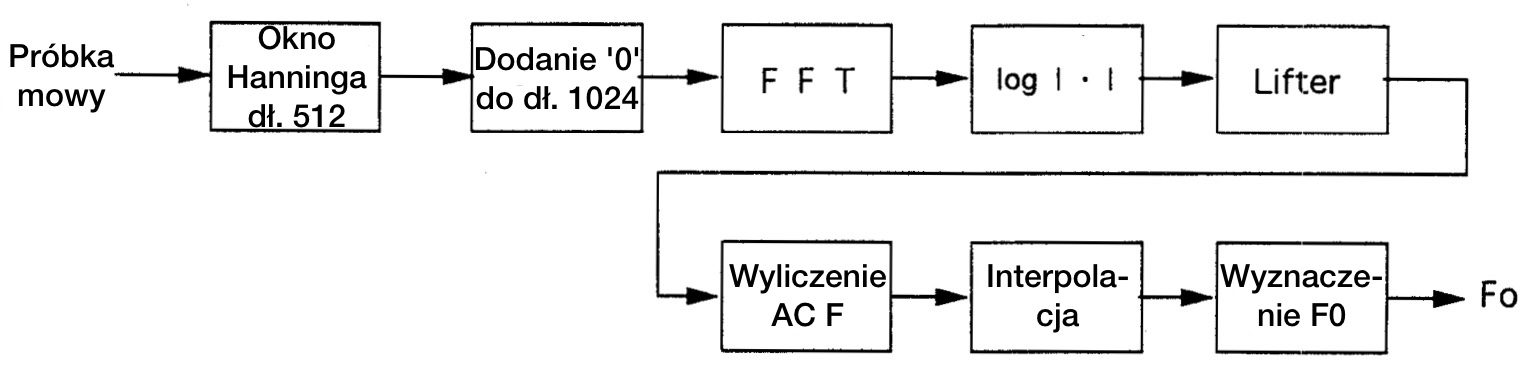
\includegraphics[scale=0.29]{images/ACLOS/ACLOS_flow.jpg}
    \caption{Schemat działania algorytmu ACLOS do wykrywania wysokości dźwięku. Schemat z 
    \cite[233]{Transcription:Kunieda:Aclos}
    %\cite[r. 2]{Transcription:Kunieda:Aclos}
    .}
    \label{fig:aclos:flow}
  \end{center}
\end{figure}

Nazwa algorytmu ACLOS jest skrótem \textit{AutoCorrelation of LOg Spectrum}, co oznacza autokorelację na logarytmie widma (tłumaczenie własne). Motywacją do stworzenia ACLOS było odkrycie takiego algorytmu, który wykorzysta zalety cepstrum i jednocześnie będzie bardziej odporne na szumy w badanym sygnale. Dodatkowo, autorzy ACLOS przytaczają prace naukową \cite{Transcription:Lahat:SpectralAutocorrelationNoiseCorrupted}, która również wykorzystuje autokorelacje na widmie sygnału akustycznego, z tą różnicą, że nie stosuje się na nim logarytmowania, a proces autokorelacji determinowany jest procedurą decyzyjną zależną od pików na poszczególnych pasmach sygnału, co czyni ten algorytm dużo bardziej złożony niż ACLOS.

\begin{figure}[h]
  \begin{center}
    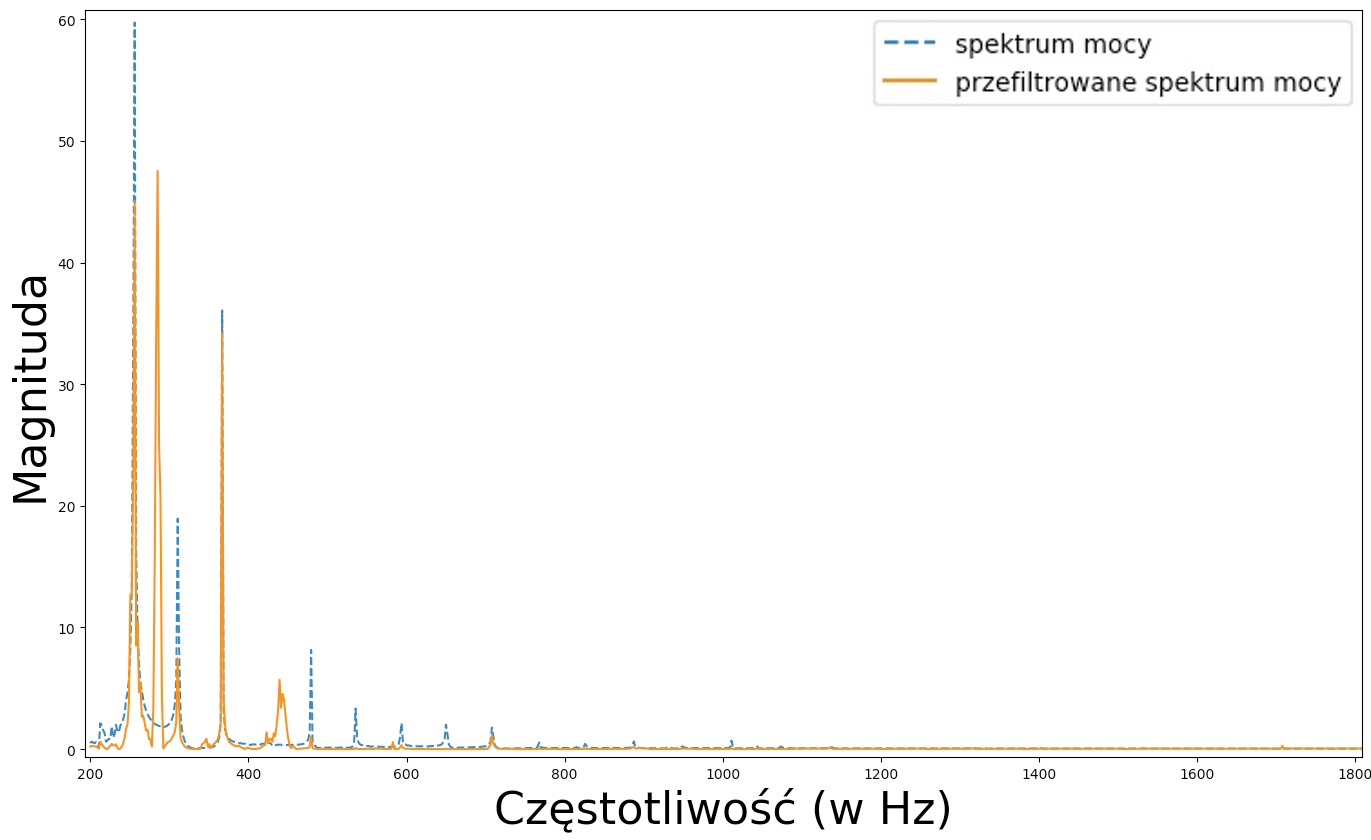
\includegraphics[scale=0.33]{images/ACLOS/data_lifter_cropped.jpg} 
    \caption{Wykres przedstawiający spektrum na pojedyńczym oknie przed i po nałożeniu lifterowania ze współczynnikiem równym 10} 
    \label{fig:aclos:lifter}
  \end{center}
\end{figure}

Schemat działania algorytmu ACLOS dla okna Hanninga o długości 512 sampli przedstawiony jest na rysunku \ref{fig:aclos:flow}. W zależności od długości okna zmieniać się będzie wynikowa częstotliwość i maksymalna częstotliwość, jaką można wykryć w sygnale (zgodnie z równaniem Nyquista przedstawionym w \ref{eq:NyquistFq}). Do okna dodana jest odpowiednia ilość zer jako margines, które mają na celu zwiększenie częstotliwości widma (jak zostało opisane w sekcji \ref{sec:przetwarzanieFFT}). W oryginalnej pracy margines ten ma długość 512, aby wynikowe okno miało długość równą 1024. Na rozszerzonym o wektor zer oknie wyliczana zostaje szybka transformata fouriera, a z niej wynik przetwarzany jest do logarytmu spektrum mocy zgodnie ze wzorem \ref{eq:powSpec}. Następną operacją, jaka jest wykonywana na analizowanych danych, jest filtrowanie w domenie cepstrum. Liftering ma tu na celu wyrównanie spektrum i zmniejszenie wpływu, jaki ma na wynik szum. Wynik działania lifteringu można zaobserwować na wykresie rysunku \ref{fig:aclos:lifter}. Na tak przygotowanym oknie wykonywana jest funkcja autokorelacji $R(j)$, która ma postać:
\begin{align}\label{eq:Aclos:ACf}
  R(j)& = \frac{1}{N}\sum_{i=0}^{N-1}f(i)f(i + j)&
  j = 0, 1, ..., M
\end{align}
gdzie $f(i)$ jest i-tym komponentem lini widmowej, $N$ oznacza zakres harmonicznych, który brana jest pod uwagę, $j$ jest częstotliwością dla której badany jest współczynnik autokorelacji a $M$ oznacza maksymalną częstotliwość, jaką może posiadać F0 w analizowanym sygnale 
\cite[50-51]{Transcription:Quenneville:Thesis}
%\cite[r. 5.3.2]{Transcription:Quenneville:Thesis}
.

\begin{figure}[ht]
  \begin{subfigure}{.49\textwidth}
    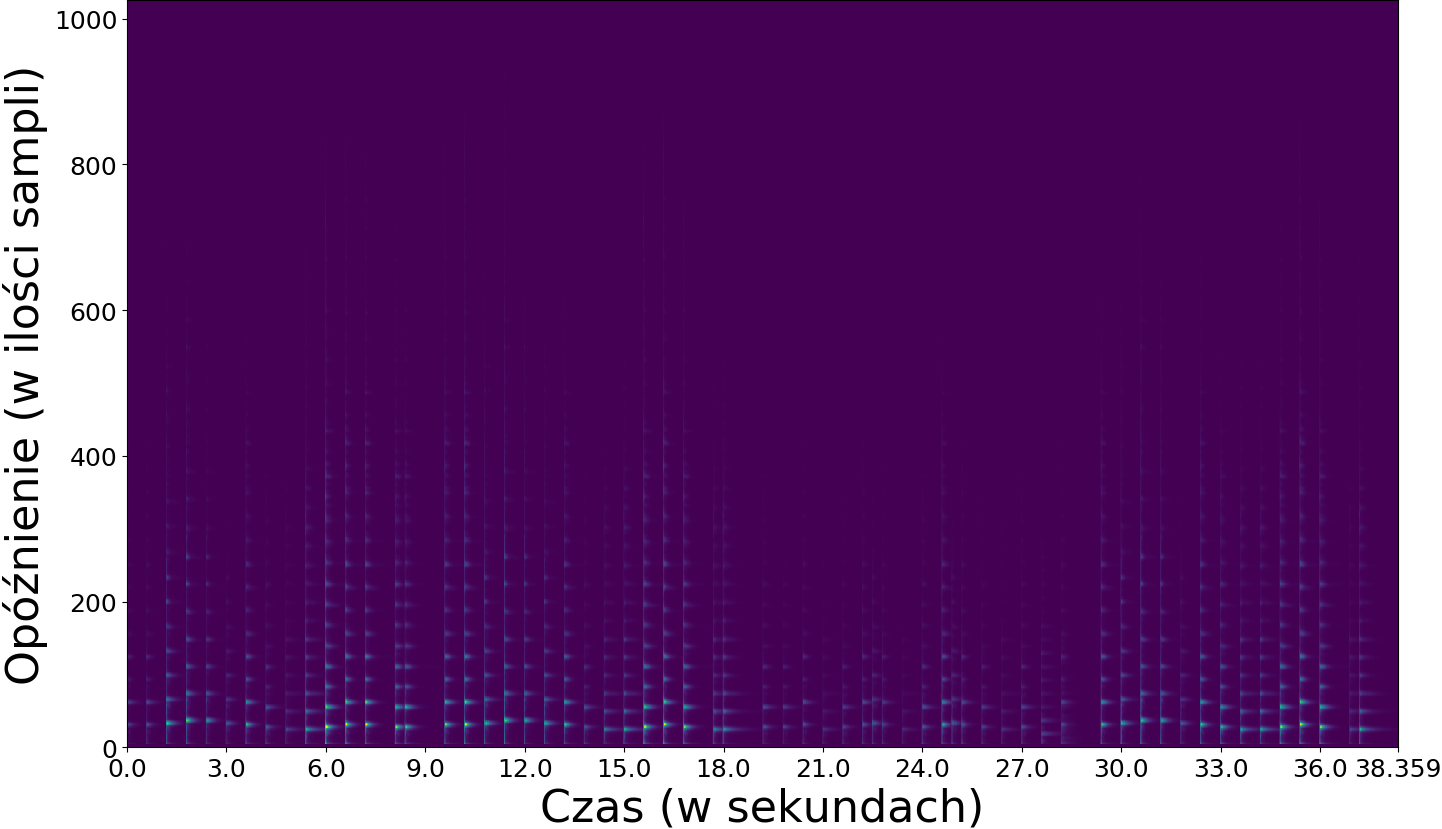
\includegraphics[width=1.\linewidth]{images/ACLOS/Korelogram_cropped.png}
    \caption{Korelogram}
  \end{subfigure}
  \begin{subfigure}{.5\textwidth}
    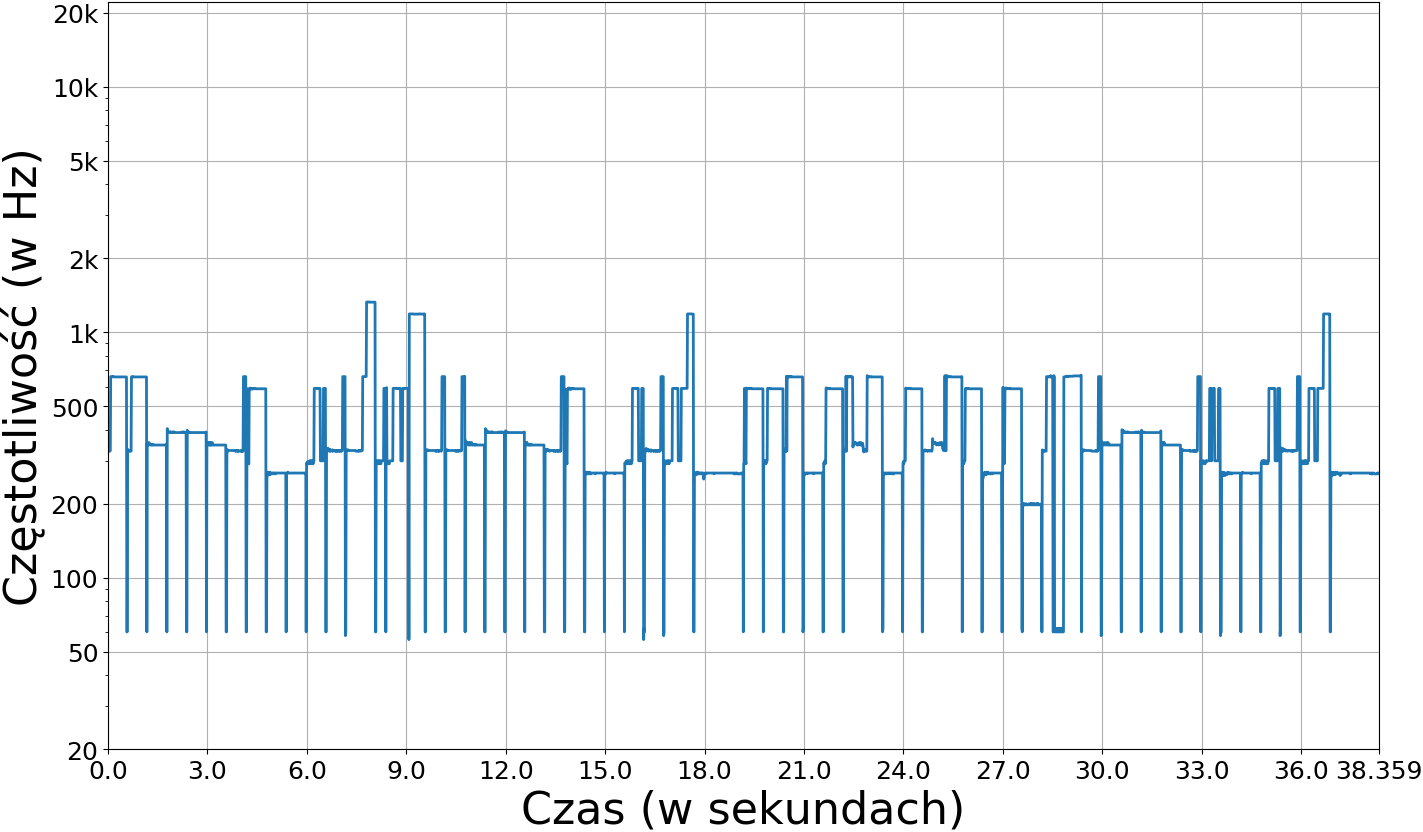
\includegraphics[width=1.\linewidth]{images/ACLOS/Estymacja_f0_cropped.png}
    \caption{Estymacja F0}
  \end{subfigure}
  \newline
  \begin{subfigure}{0.5\textwidth}
    \centering
    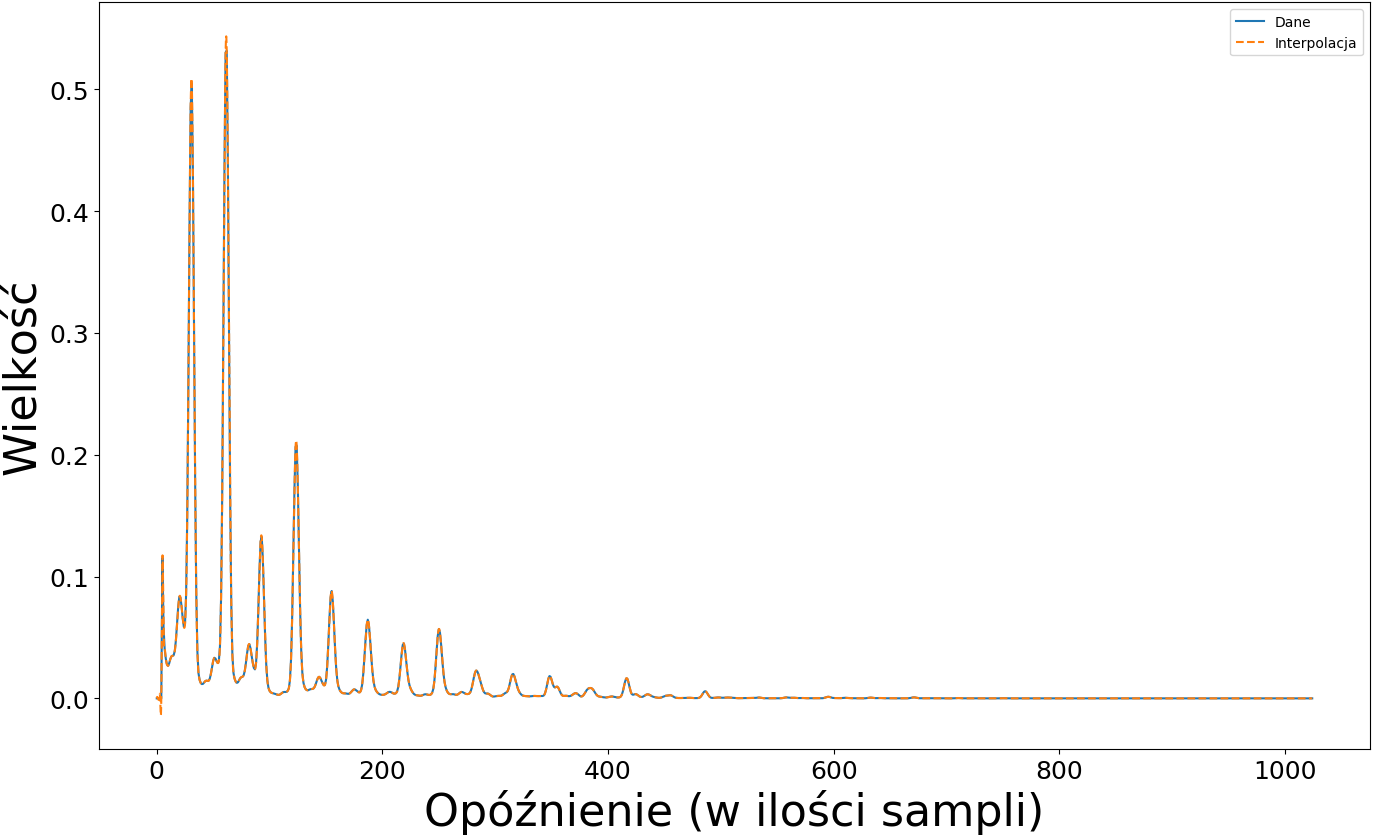
\includegraphics[width=1.\linewidth]{images/ACLOS/interpolacja_full_cropped.png}
    \caption{Okno autokorelacji i jego interpolacja}
  \end{subfigure}
  \begin{subfigure}{0.49\textwidth}
    \centering
    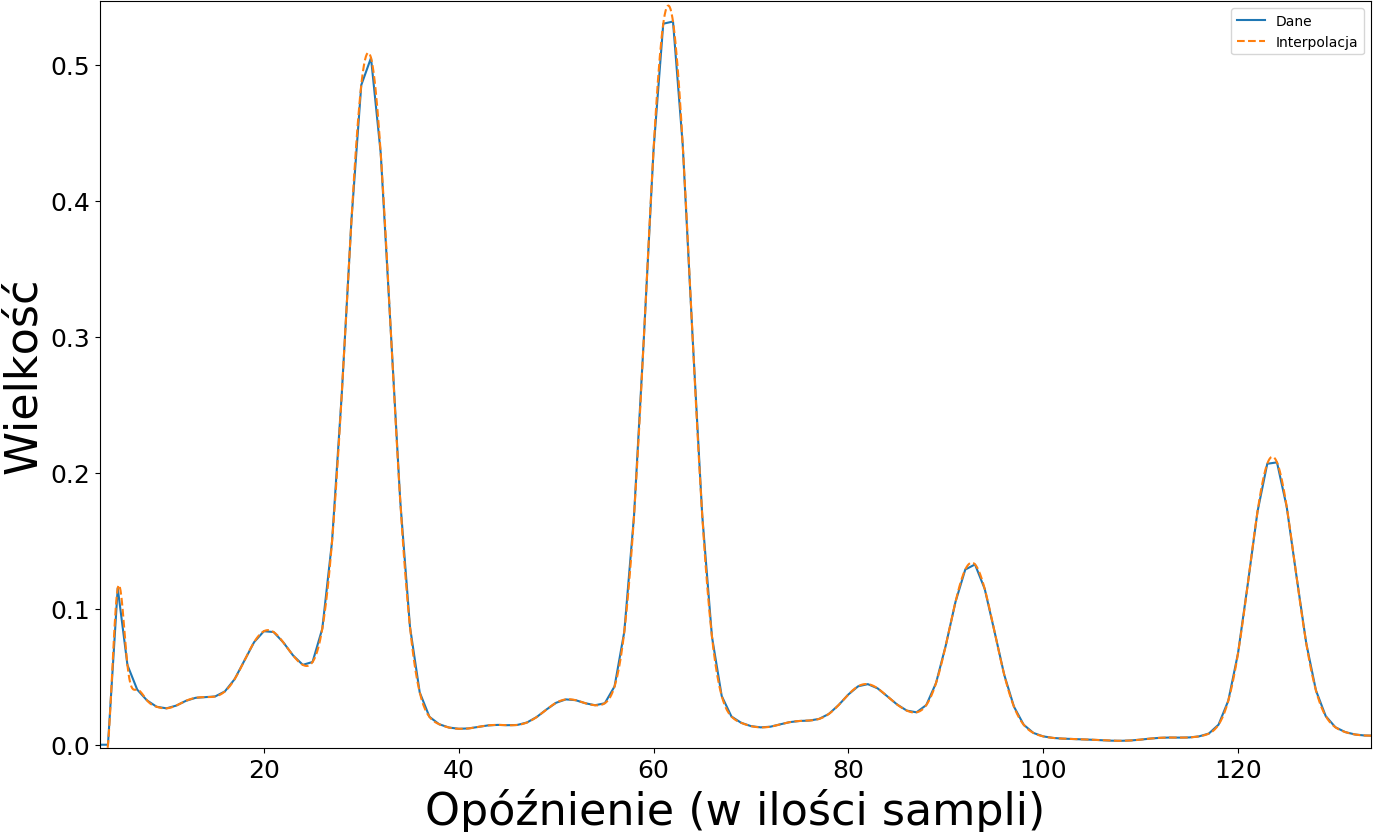
\includegraphics[width=1.\linewidth]{images/ACLOS/Interpolacja_superzoomed_cropped.png}
    \caption{Wykres (c) w przybliżeniu}
  \end{subfigure}
  \caption{Wynik ACLOS użytego na kompozycji ,,Oda do radości'' IX symfonii Beethovena zagranej monofonicznie na pianinie. Użyto okno Hanna o długości 2048 sampli z odstępami długości 512 sampli. Wykresy (c) i (d) przedstawiają wynik równania \ref{eq:Aclos:ACf} na tym samym oknie po zastosowaniu lifteringu. Jaśniejsze obszary w cepstrogramie oznaczają większa magnitudę.}
  \label{fig:aclos:results}
\end{figure}

Algorytm ACLOS po wyliczeniu wektora autokorelacji dla danego okna zakłada wyznaczenie F0 na podstawie maksymalnego wyniku \ref{eq:Aclos:ACf}. Szerokość pasma pojedyńczego spektralnego komponentu zależna jest od przyjętej długości okna, a pasmo to jest zakresem, w którym znajduje się znalezione F0. Autorzy używają interpolacji wokół wartości wyznaczonej przez autokorelacje, co w rezultacie umożliwia uzyskanie większej dokładności wyniku. Możliwości użycia autokorelacji w metodykach wykrywania F0 zostały pokazane między innymi w pracy 
\cite[1046-1047]{Transcription:Suzuki:EstimationOfMistunedFrequency}
%\cite[r. 3-4]{Transcription:Suzuki:EstimationOfMistunedFrequency}
.

Wyniki ACLOS w wyznaczaniu F0 są podobne do tych, wyznaczonych przez metodę Cepstrum (\ref{sec:f0:ceps}) co można zaobserwować na rysunku \ref{fig:aclos:results}. Większa niedokładność na początku kolejnych wysokości jest spowodowana charakterystyką użytego pianina, którego barwa podczas narastania amplitudy dźwięku jest nieliniowa. ACLOS jest uważane za metodę bardziej odporną na szum w analizowanym sygnale niż metoda Cepstrum \cite{Transcription:Kunieda:Aclos}.

\newpage
\section{Estymacja wielu częstotliwości fundamentalnych w sygnale polifonicznym}\label{sec:MultiPitch}
Ten rozdział skupia się na opisaniu metod estymacji składowej fundamentalnej w polifonicznym sygnale akustycznym. Sygnał polifoniczny to taki, w którym występują co najmniej dwa równoległe dźwięki w tym samym czasie. Problem ten jest znacznie bardziej złożony od wyznaczania pojedyńczego F0 opisanego w \ref{sec:f0}. Wiele z własności sygnałów akustycznych, jak periodyczność czy rozróżnialna barwa, nie są niezawodnym źródłem informacji w celach transkrypcji wielotonowej, ponieważ nakładające się na siebie dźwięki modulują te cechy dźwięków zniekształcając ich pierwotną formę.

Współczesna muzyka zachodnia jest w dużym stopniu ustrukturyzowana zarówno w domenie czasu jak i częstotliwości. Tempo i rytm, w którym dany utwór jest grany, są informacjami zawartymi w domenie czasu. Dzięki wzorcom, które są zachowywane w muzyce, można te informacje wywnioskować. W domenie częstotliwości natomiast widoczne są zależności pomiędzy poszczególnymi wysokościami dźwięków. Pojedyńczej zagranej nucie towarzyszy, poza częstotliwością fundamentalną, szereg wydźwięków, co było już wielokrotnie udowadniane, jak na przykład w 
\cite[1325-1326]{Transcription:Mcintyre:OnTheOscilation}
%\cite[sekcja INTRODUCTION]{Transcription:Mcintyre:OnTheOscilation}
. Wibracje te badane przez fizyków były dostosowywane tak, aby pasowały do modeli normalnych. Ich struktura częstotliwości różni się w zależności od użytego instrumentu i sposobu w jaki został zagrany dźwięk. Częstotliwość i rozmieszczenie harmonicznych jest odgórnie ustalone przez instrument i sposób w jaki została zagrana nuta. Pomimo, że harmoniczne zawsze posiadają pewne odchylenie od perfekcyjnej harmonii (nie są dokłądną algebraiczną wielokrotnością częstotliwości F0, a oscylują w jej okolicy) dla konkretnego instrumentu i sposobu zagrania będą odgórnie zdefiniowane przez pewien model matematyczny 
\cite[1326-1327]{Transcription:Mcintyre:OnTheOscilation}
%\cite[r. 1]{Transcription:Mcintyre:OnTheOscilation}
. Jak opisuje Manuel Davy w 
\cite[203-204]{Transcription:Anssi:SignalProcessingMethods} 
%\cite[r. 7]{Transcription:Anssi:SignalProcessingMethods} 
struktura muzyki tonalnej może zostać wykorzystana do budowy modeli bayesowskich, czyli modeli matematycznych w kontekście probabilistycznym, które prowadzą do najprostszego modelu wyjaśniającego daną fale dźwiękową. Pomimo tego, że modele te wydają się naturalnym rozwiązaniem estymacji wielotonowej, ponieważ rozwiązują problem dużej ilości parametrów w fali dźwiękowej, których nie można wyestymować beż pewnych założeń, nie są one często wykorzystywane. Przytoczona wcześniej praca \cite{Transcription:BayesianHarmonicModels} jest przykładem wykorzystania modeli bayesowskich do analizowania sygnałów muzycznych, w tym wykrywania F0.

\subsection{Wyniki algorytmów do sygnałów monofonicznych}\label{sec:MultiPitch:monofon}
W rozdziale \ref{sec:f0} struktura częstotliwości rozumiała była jako obraz pojedyńczej częstotliwości fundamentalnej, z którego jednoznacznie wynika, jaka wysokość dźwięku jest grana w danym momencie czasu. Duża większość muzyki jest polifoniczna i tylko momentami skomplikowane kompozycje dopuszczają się brzmienia jedynie pojedynczych nut. W takich utworach metodologie transkrypcji muzyki monofonicznej są nieefektywne.

\begin{figure}[ht]
  \begin{center}
    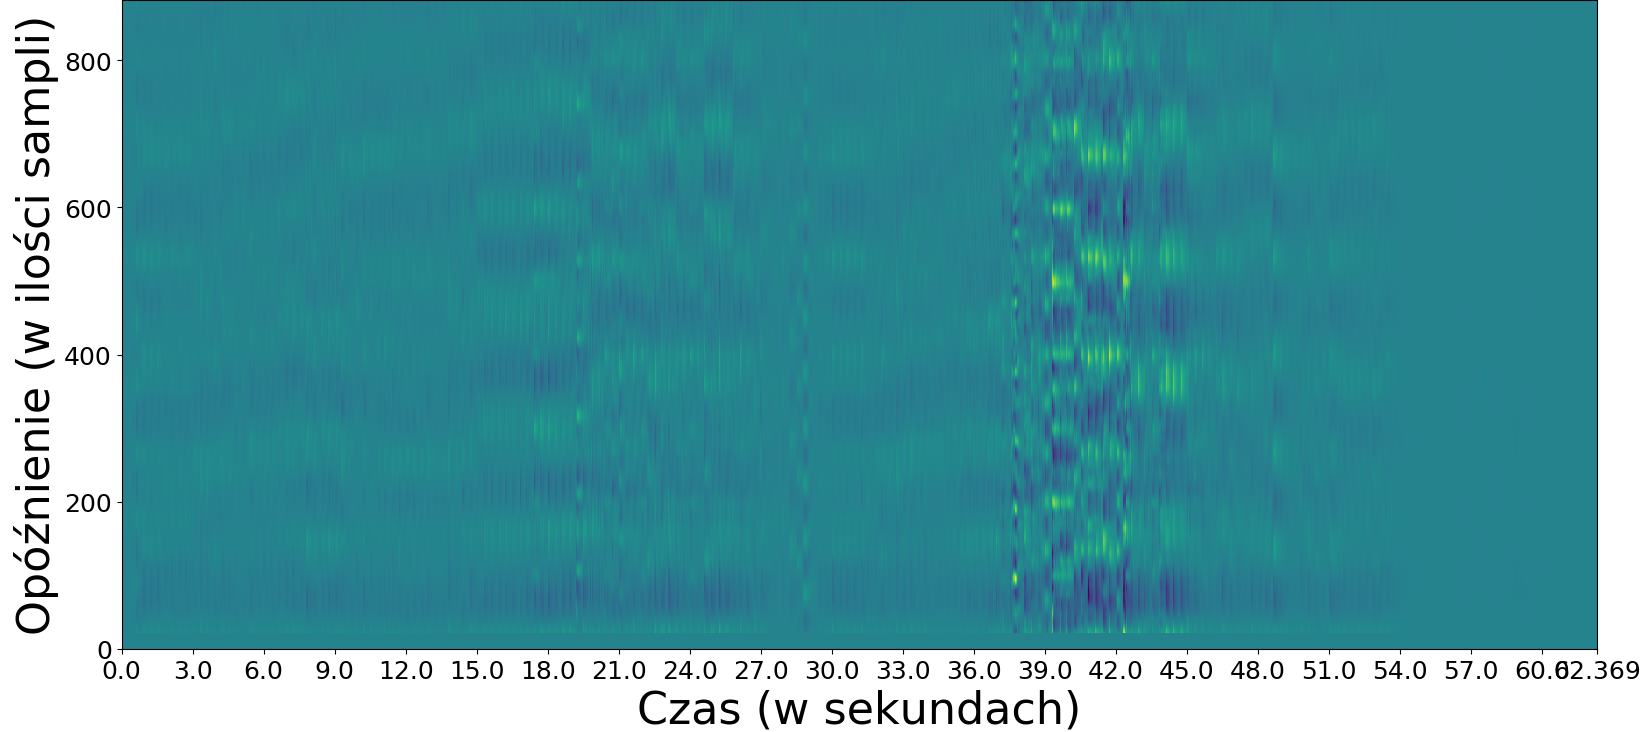
\includegraphics[scale=0.38]{images/AC/korelogram_multif0_cropped.png}
    \caption{Funkcja autokorelacji \ref{eq:AC} zastosowana na nagraniu Preludium op. 28 nr. 4 Fryderyka Chopina zagranym na pianinie w Em. Użyto okno Hanna o długości 2048 sampli z odstępami długości 2048 sampli.}
    \label{fig:multi:ac}
  \end{center}
\end{figure}

Funkcja autokorelacji w domenie czasu/mocy, jak opisana w sekcji \ref{sec:f0:ac} polegała na znalezieniu powtarzalności w fali dźwiękowej. Ta cykliczność była bezpośrednim efektem periodyczności pojedyńczych dźwięków. Gdy w tym samym czasie granych jest więcej nut, nawet na pojedyńczym instrumencie, AC nie jest w stanie odróżnić ich od siebie. Na rysunku \ref{fig:multi:ac} przedstawiony jest korelogram, wygenerowany analogicznie do korelogramu na rysunku \ref{fig:ACResults:corr} z tą różnicą, że sygnał bazowy jest tu polifoniczny. Rezultat jest niejednoznaczny i nie można na jego podstawie wnioskować żadnej z dźwięków granych w utworze.

\begin{figure}[ht]
  \begin{subfigure}{1.\textwidth}
    \centering
    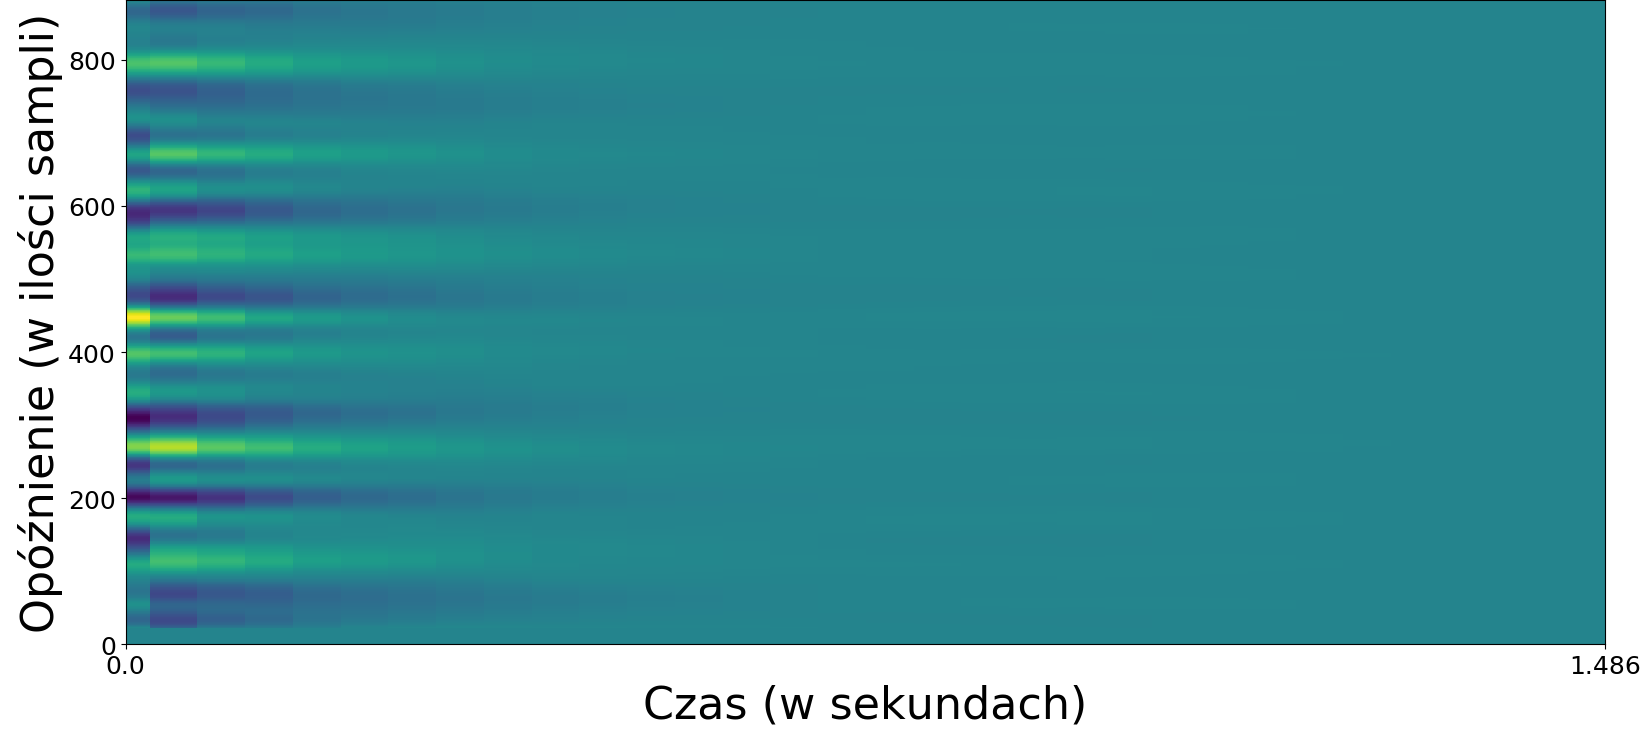
\includegraphics[width=.49\linewidth]{images/Em/Corelogram_cropped.png}
    \caption{Korelogram}
  \end{subfigure}
  \newline
  \begin{subfigure}{0.5\textwidth}
    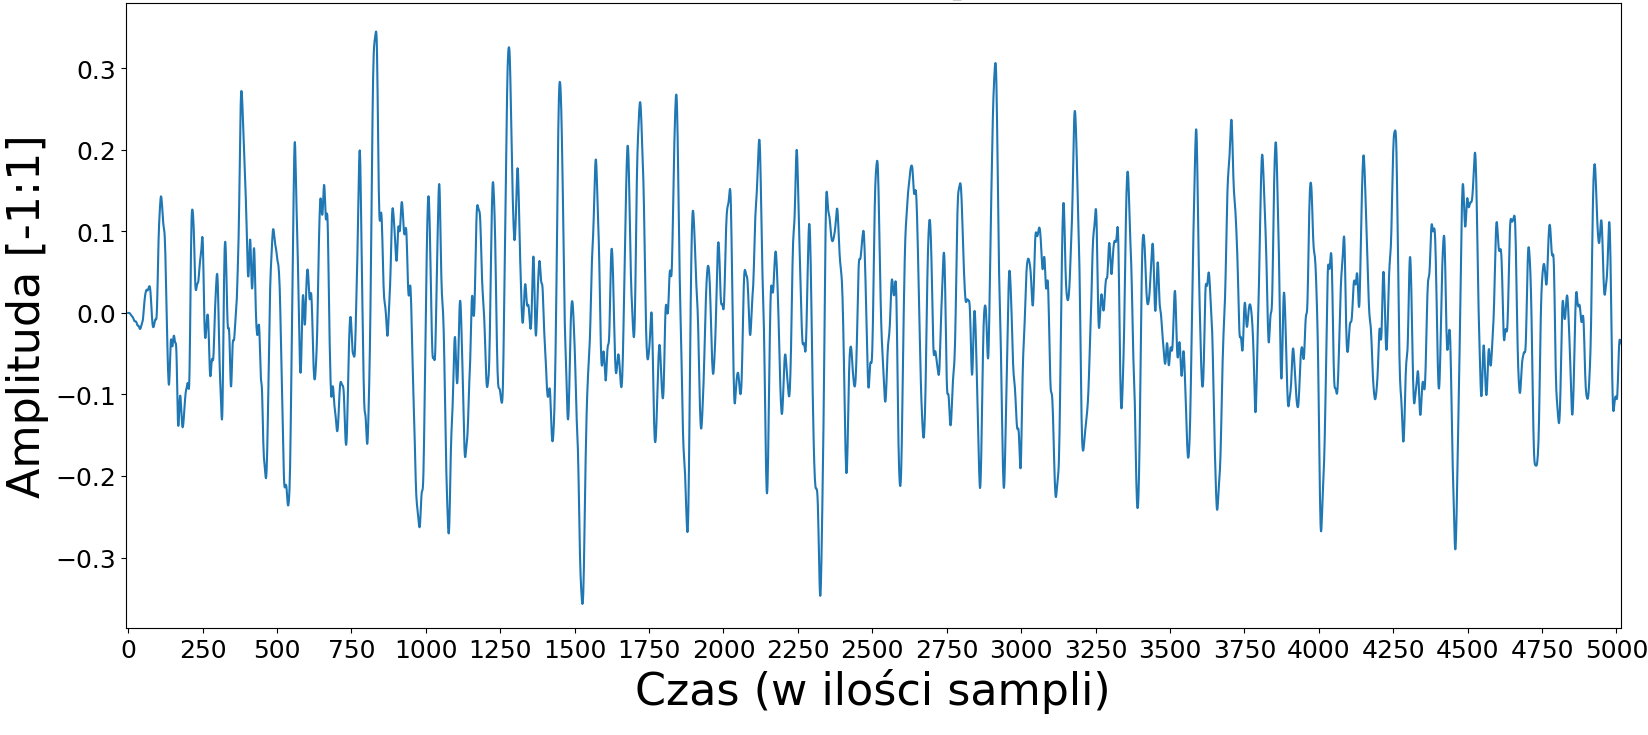
\includegraphics[width=1.\linewidth]{images/Em/waveform_zoom_samples_cropped.png}
    \caption{Sygnał fali dźwiękowej w przybliżeniu}
  \end{subfigure}
  \begin{subfigure}{0.49\textwidth}
    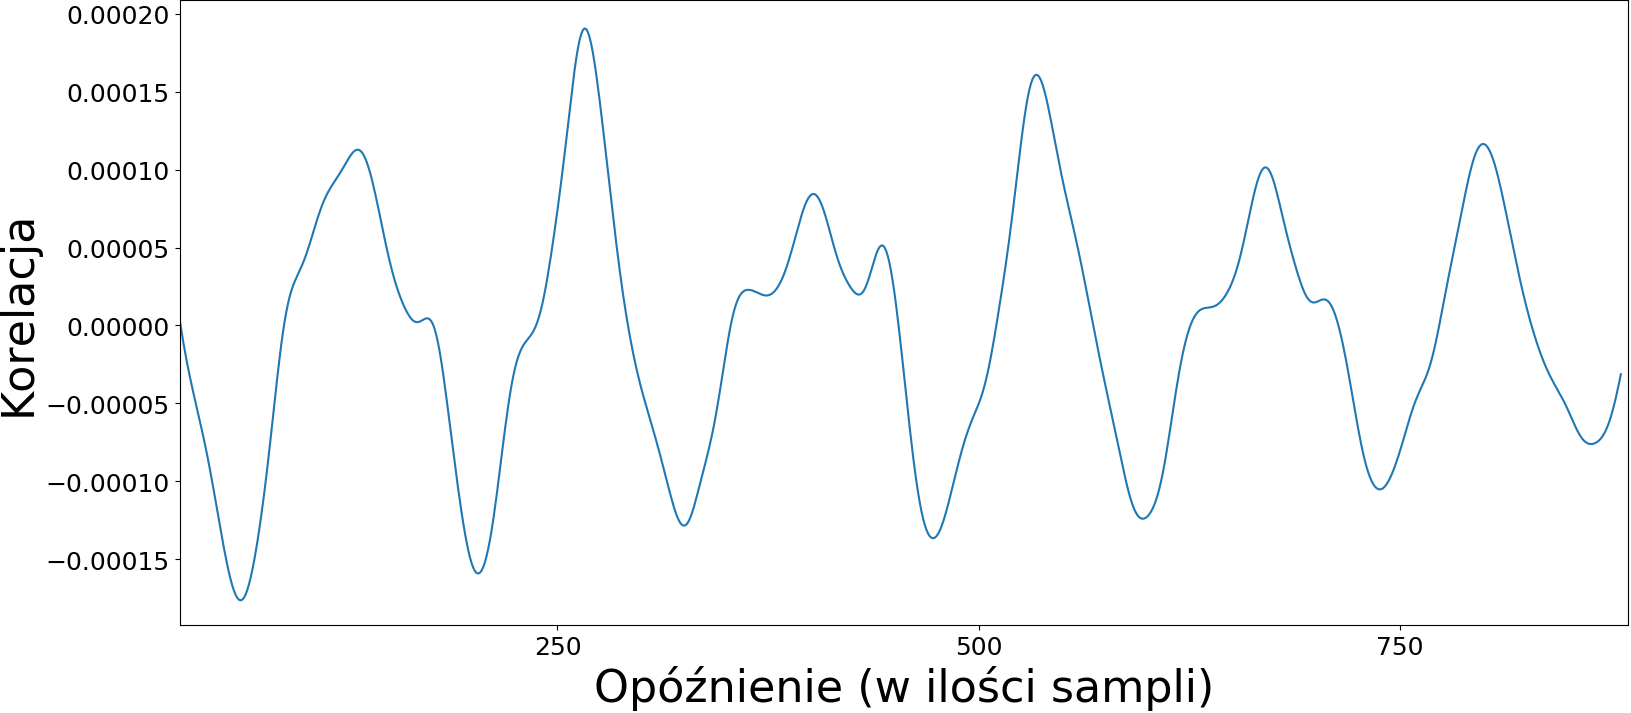
\includegraphics[width=1.\linewidth]{images/Em/corelation_cropped.png}
    \caption{Wykres autokorelacji okna danych}
  \end{subfigure}
  \caption{Wynik funkcji autokorelacji na nagraniu akordu Em zagranym na pianinie. Użyto okno Hanna o długości 2048 sampli z odstępami długości 2048 sampli. Wykresy (c) jest reprezentacją wyników AC na 11 oknie (próbce danych od 20480 do 22528 sampli z sygnału wejściowego).}
  \label{fig:multi:ac:em}
\end{figure}

Przyglądając się z bliska pojedyńczemu wynikowi funkcji autokorelacji jak widać na rysunku \ref{fig:multi:ac:em} można zauważyć, że piki znajdują się w nieregularnych odstępach, a sama wartość funkcji korelacji nie jest bliska maksymalnej wartości. Na omawianej ilustracji grany jest akord E-mol 3, czyli dokładnie dźwięki E3, G3 i B3, którym odpowiadają częstotliwości F0 odpowiednio 164.81, 196.00 i 246.94 Hz. W badanym oknie korelacji najwyższy pik jest w miejscu o przesunięciu 266, czyli najsilniejszą hipotezą co do F0 byłaby częstotliwość 165,8 Hz (zgodnie ze wzorem \ref{eq:AC:hz} w badanym przypadku częstotliwość wyliczana jest poprzez $44100 / 266 \approx 165,8$), co jest wartością najbliższą do częstotliwości dźwięku E3. Najniższa nuta w akordzie nazywana jest bazową, i to ona jest najbardziej charakterystyczna dla ludzkiego ucha. Z racji tego, że ma ona najniższą częstotliwość, ma też najwyższą amplitudę (z reguły im wyższa częstotliwość tym niższa amplituda), co daje wyższą szanse na znalezienie tych nut w dźwięku przy wykorzystaniu funkcji autokorelacji w domenie czasu. Drugi pik pod względem rezultatu autokorelacji jest dla przesunięcia równego 534, co odpowiada częstotliwości równej 52,6 Hz. Ta częstotliwość nie jest częścią granego dźwięku, nie jest również żadna z jej wielokrotności.

\begin{figure}[ht]
  \begin{center}
    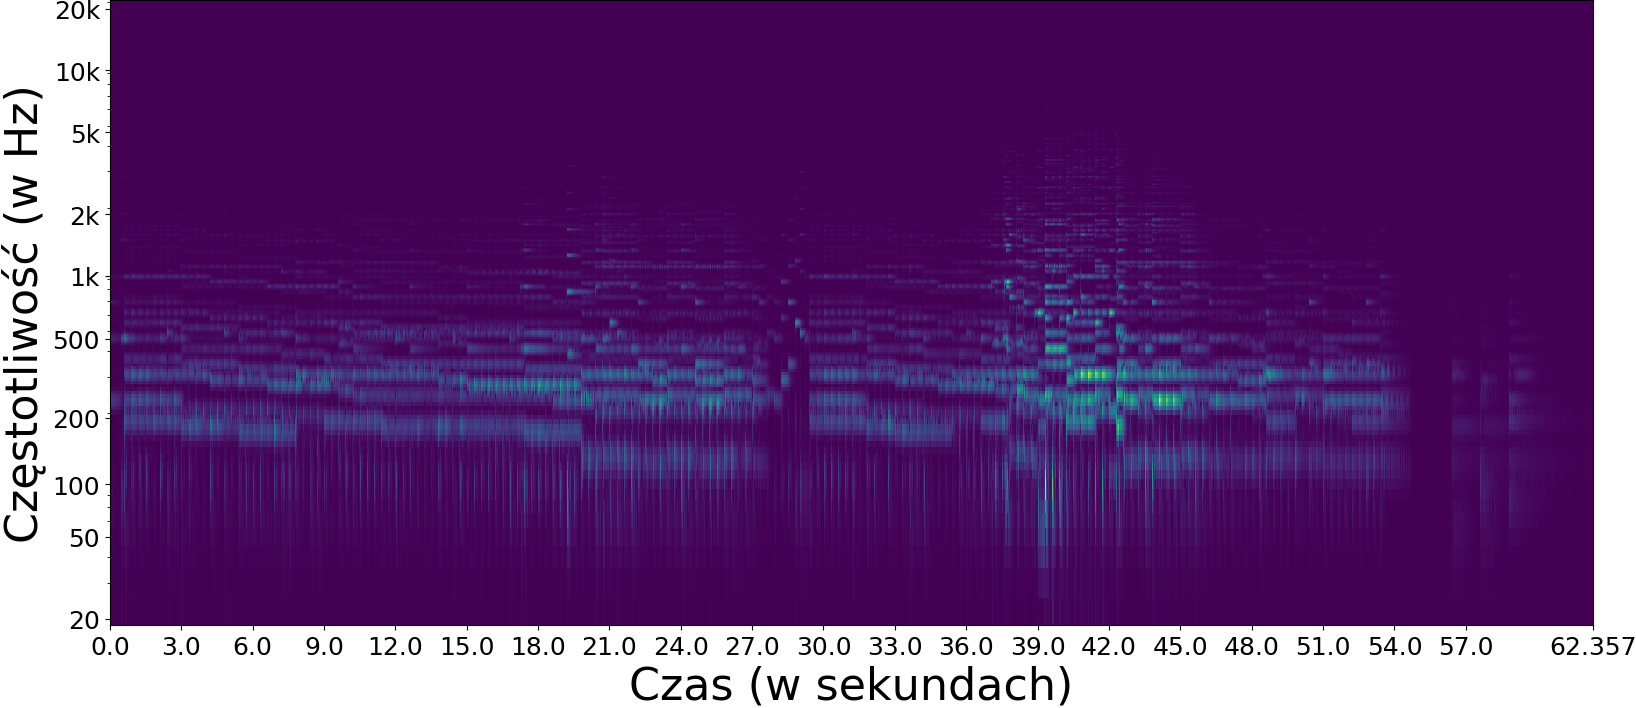
\includegraphics[scale=0.38]{images/Spectrogram/spectrogram_multi_2048_512_cropped.png}
    \caption{Spektrogram nagrania Preludium op. 28 nr. 4 Fryderyka Chopina zagranym na pianinie w Em. Użyto okno Hanna o długości 2048 sampli, marginesem zer o długości 2048 i z odstępami długości 512 sampli. Jaśniejsze obszary w spektrogramie oznaczają większa magnitudę.}
    \label{fig:multi:spectrogram}
  \end{center}
\end{figure}

Metody operujące na dziedzinie częstotliwości mają dużo większą skuteczność w wykrywaniu równoległych F0, jednak algorytmika stojąca za tymi metodami jest dużo bardziej skomplikowana niż w przypadku monofonicznych utworów ze względu na dużo bardziej złożone widma. Spektrogram sygnałów polifonicznych nie jest tak wyraźnym wskaźnikiem jak był w przypadku monofonicznym. Częstotliwości harmonicznych mogą się na siebie nakładać, zniekształcając ich cykliczność jak i modulując wyraźność formantów.

\begin{figure}[H]
  \begin{center}
    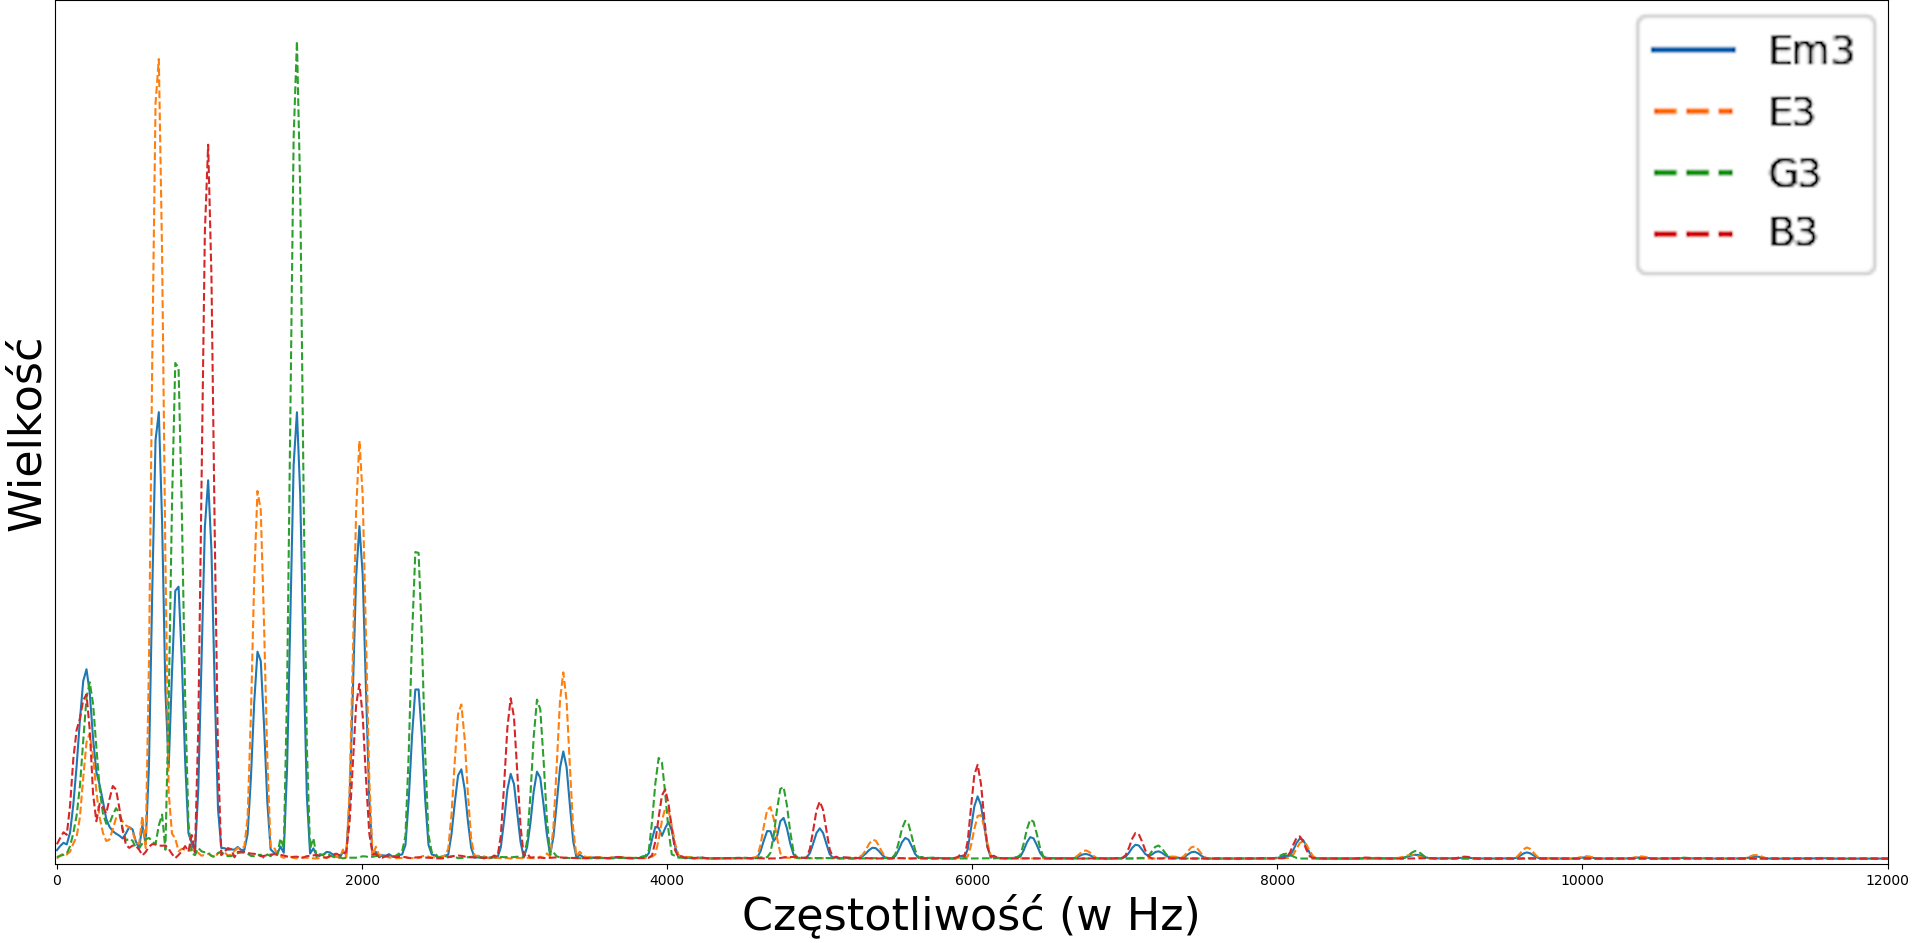
\includegraphics[scale=0.325]{images/Em/spectral_component_em3_partials_2048_512_cropped.png}
    \caption{Spektralne komponenty nagrania akordu Em zagranego na pianinie oraz trzech poszczególnych nut zagranych na tym samym pianinie nagranych osobno. Użyto okna Hanna o długości 2048 sampli i marginesu zer długości 2048.}
    \label{fig:multi:spectra:partials}
  \end{center}
\end{figure}

\begin{figure}[H]
  \begin{center}
    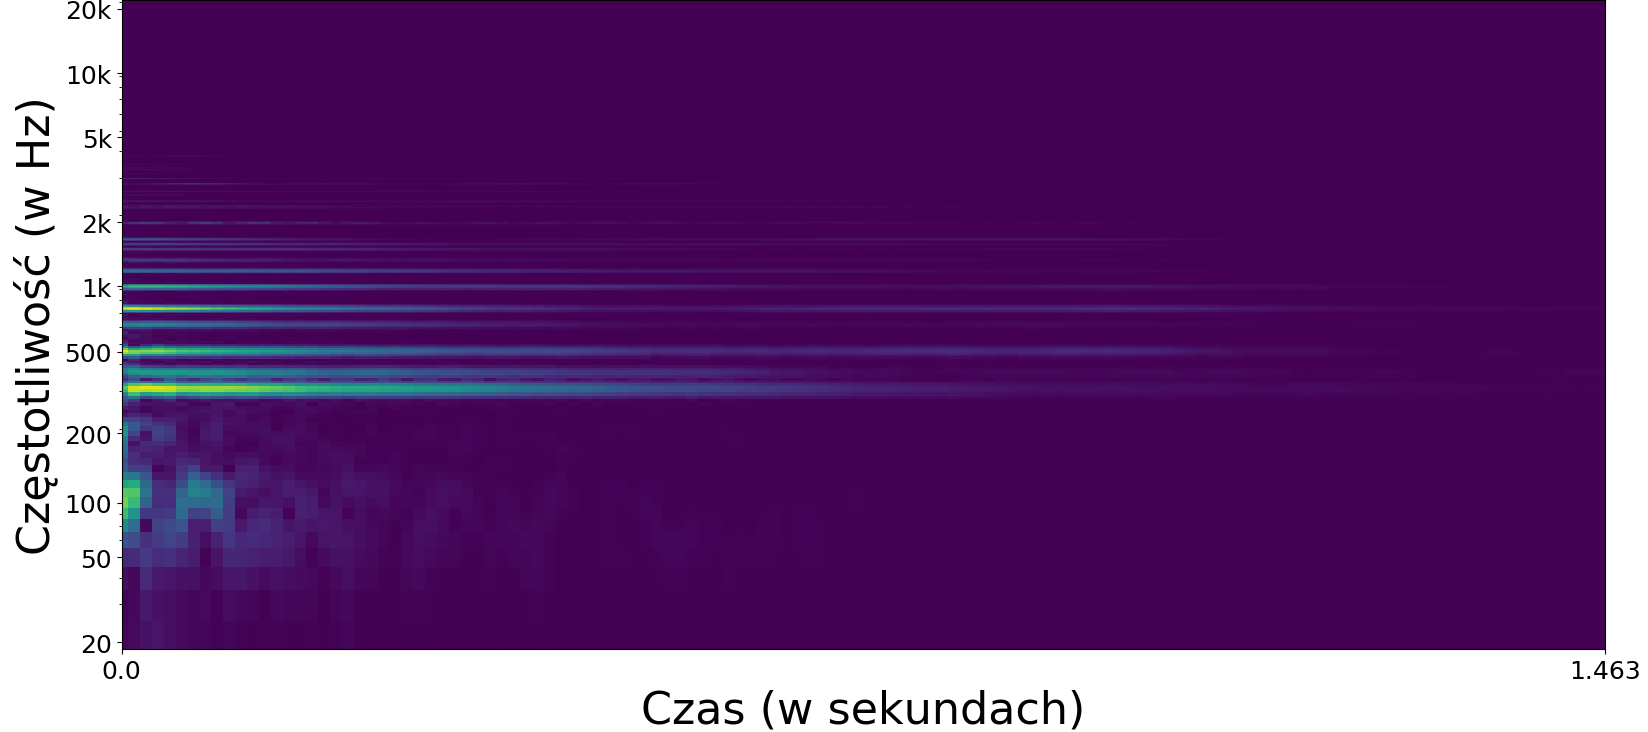
\includegraphics[scale=0.27]{images/Em/spectrogram_Em_2048_512_cropped.png}
    \caption{Spektrogram nagrania akordu Em zagranego na pianinie. Użyto okna Hanna o długości 2048 sampli z marginesem zer długości 2048 i marginesu zer długości 2048. Jaśniejsze obszary w spektrogramie oznaczają większa magnitudę.}
    \label{fig:multi:em:spectrogram}
  \end{center}
\end{figure}

Widma poszczególnych dźwięków nakładają się na siebie, wzmacniając pewne częstotliwości, a inne wytłumiając. Przykład takiego zjawiska można zaobserwować na rysunku \ref{fig:multi:spectra:partials}. Nagranie akordu Em3 zagranego na pianinie widać linią ciągłą, natomiast pojedyńczo nagrane dźwięki E3, G3 oraz B3 są przedstawione jako osobne krzywe. Widać na tym wykresie, że wynikowa krzywa Em żadko nakłada się dokłądnie z linią pojedyńczej nuty, a jest raczej nową strukturą z częścią cech wspólnych.

Metody cepstrum i ACLOS opisane w sekcjach \ref{sec:f0:ceps} i \ref{sec:f0:aclos} są nieefektywne z powodu nakładających się na siebie dźwięków w spektrum. Echo, które wykrywa cepstrum, jest pomieszane pomiędzy dźwiękami, co mocno komplikuje wnioskowanie z tej reprezentacji. ACLOS natomiast traci pewność wyniku z tych samych powodów co funkcja autokorelacji opisana wyżej w tej sekcji. Można zaobserwować na wykresach \ref{fig:multi:ceps:estimation} i \ref{fig:multi:aclos:estimation}, że oba te algorytmy wykryły F0 w okolicach dźwięku G (ACLOS około 190 Hz, co jest najbliższe dźwiękowi G3 obecnemu w sygnale, a Cepstrum około 400, co jest wielokrotnością G3). Przyglądając się rozbitemu na poszczególne spektra wykresowi \ref{fig:multi:spectra:partials} można wywnioskować, że nuta ta ma najwięcej wspólnych harmonicznych z pozostałymi, więc właśnie ona jest najsilniejsza w widmie.

\begin{figure}[H]
  \begin{subfigure}{0.5\textwidth}
    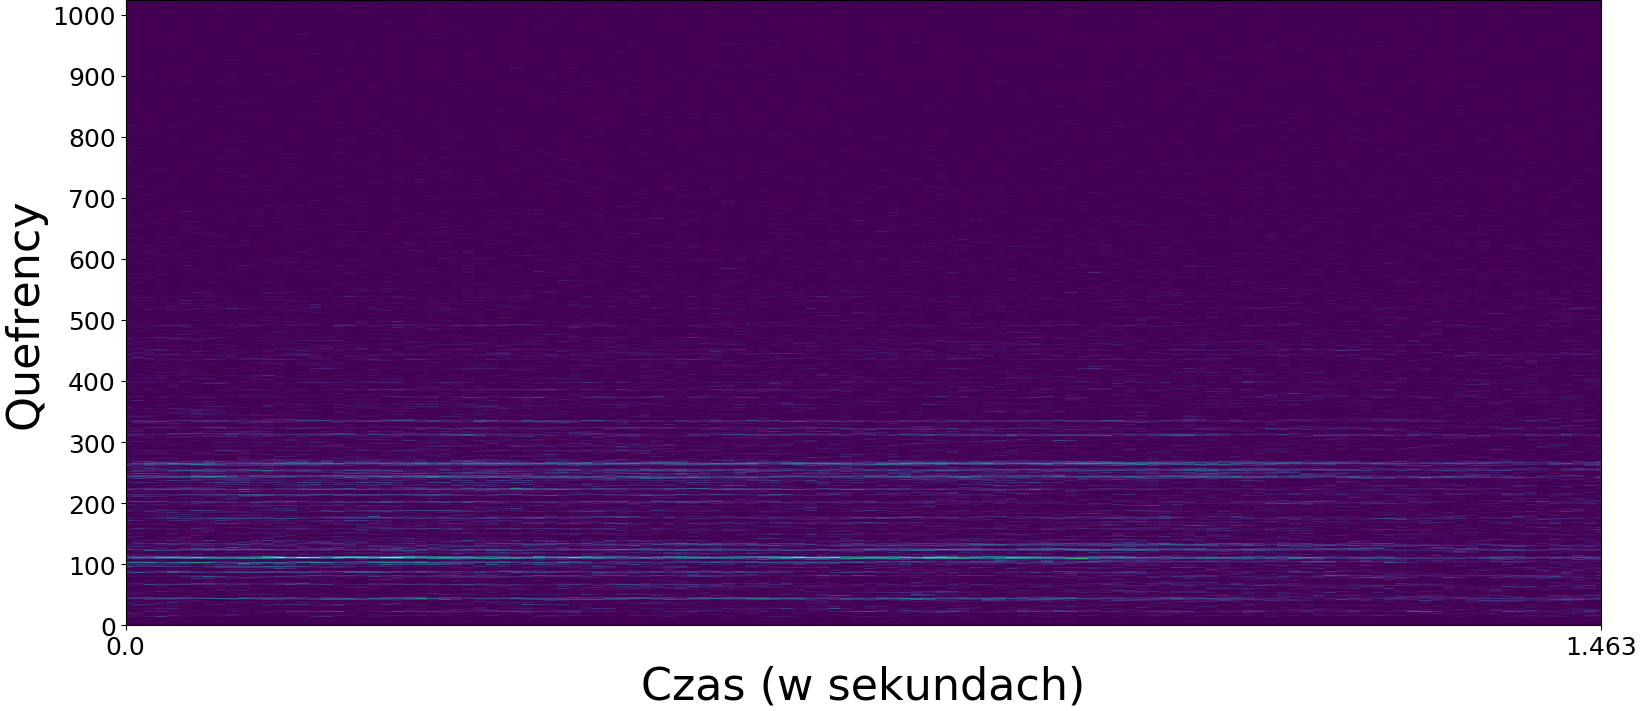
\includegraphics[width=1.\linewidth]{images/Em/cepstrogram_cropped.png}
    \caption{Cepstrogram}
  \end{subfigure}
  \begin{subfigure}{0.49\textwidth}
    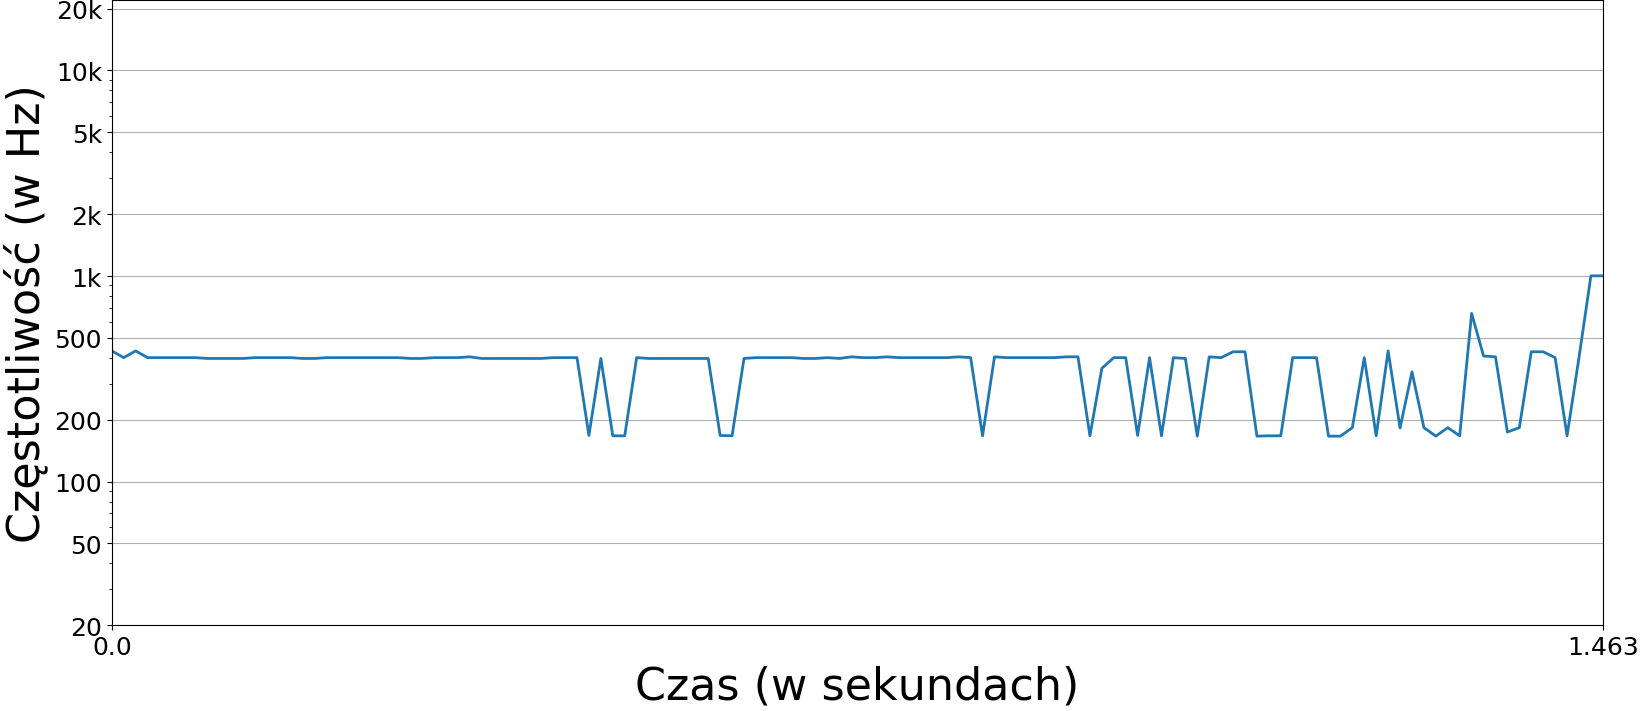
\includegraphics[width=1.\linewidth]{images/Em/cepstra_estimation_cropped.png}
    \caption{Estymacja F0}
    \label{fig:multi:ceps:estimation}
  \end{subfigure}
  \caption{Wynik cepstrum na nagraniu akordu Em zagranym na pianinie. Użyto okno Hanna o długości 2048 sampli z marginesem zer długości 2048 i odstępami długości 2048 sampli.}
  \label{fig:multi:ceps}
\end{figure}

\begin{figure}[H]
  \begin{subfigure}{0.5\textwidth}
    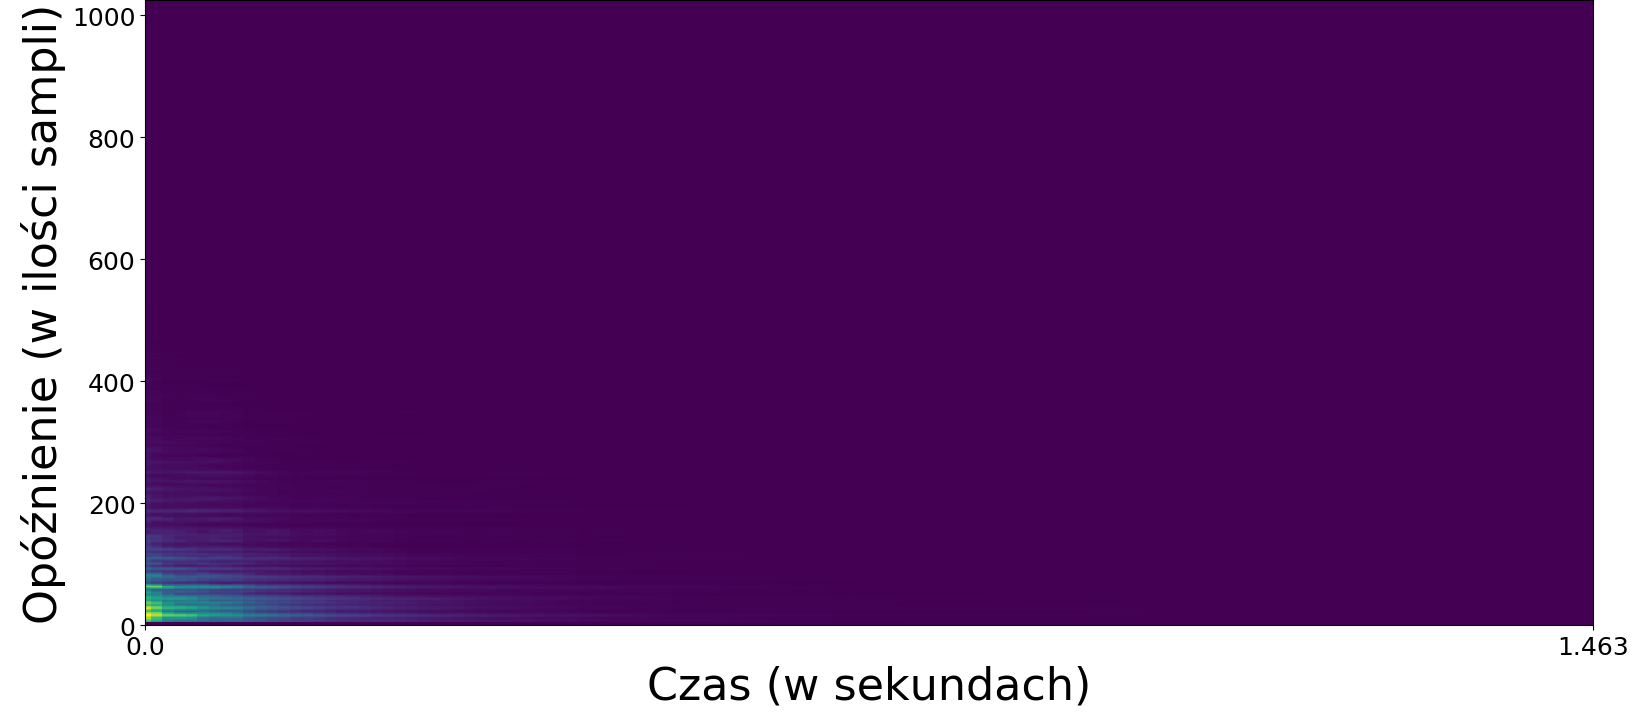
\includegraphics[width=1.\linewidth]{images/Em/Aclos_corelogram_cropped.png}
    \caption{Korelogram}
  \end{subfigure}
  \begin{subfigure}{0.49\textwidth}
    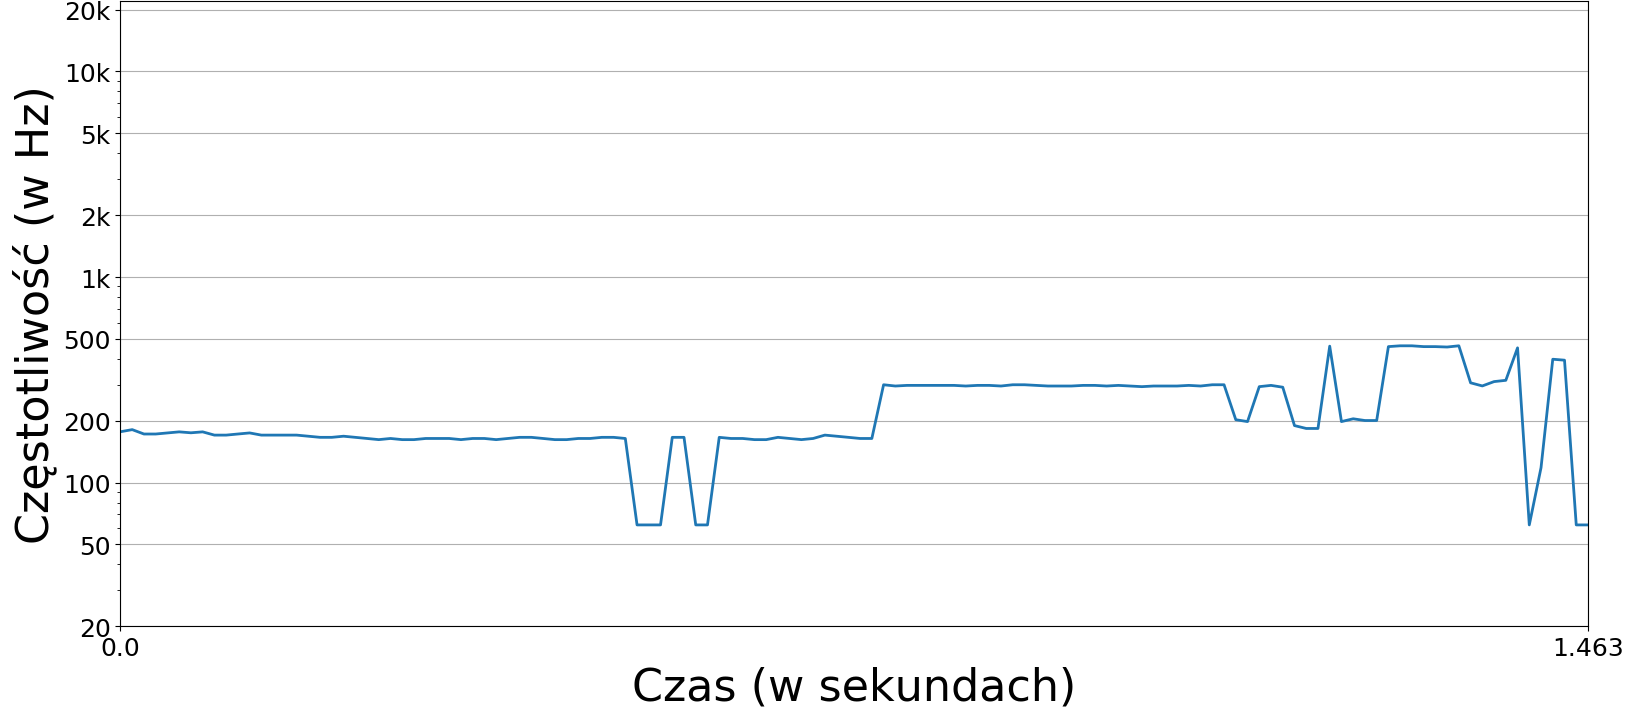
\includegraphics[width=1.\linewidth]{images/Em/Aclos_estymacja_cropped.png}
    \caption{Estymacja F0}
    \label{fig:multi:aclos:estimation}
  \end{subfigure}
  \caption{Wynik ACLOS na nagraniu akordu Em zagranym na pianinie. Użyto okno Hanna o długości 2048 sampli z marginesem zer długości 2048 i odstępami długości 2048 sampli. Jaśniejsze obszary w spektrogramach oznaczają większa magnitudę.}
  \label{fig:multi:aclos}
\end{figure}

\subsection{Metody oparte o modele generatywne}
W książce 
\cite[203-227]{Transcription:Anssi:SignalProcessingMethods} 
%\cite[r. 7]{Transcription:Anssi:SignalProcessingMethods} 
autorzy kategoryzują metodyki przeznaczone do transkrypcji częstotliwości fundamentalnych opartych na modelach generatywnych fal akustycznych ze względu na charakter algorytmu jaki jest użyty. Modele generatywne fal akustycznych czerpią z modeli bayesowskich. Rozróżnili oni metody oparte o zaszumione modele sum sinusoidów, które nie brały pod uwagę zależności pomiędzy harmonicznymi (przykładem takiego podejścia jest analiza mowy opisana w 
\cite[744-745]{Transcription:McAulay:SinusoidalRepresentationF0}
%\cite[r. 1-2]{Transcription:McAulay:SinusoidalRepresentationF0}
), oraz grupy modeli off-line i on-line.

Podejścia off-line charakteryzują się globalnym mierzeniem parametrów estymacji. Operują one analizując całą falę dźwiękową. Założeniem tych algorytmów jest segmentacja danych w taki sposób, że każdy z segmentów ma niezmienne wysokości granych dźwięków. Ograniczenie to wymusza na systemie transkrypcji użycia jakiejś formy wykrywania początków dźwięków. Algorytmy te bazują również na pojęciu prawdopodobieństwa, które to opisane jest matematycznym modelem wraz z gęstością. Algorytmy w tej grupie często działają według pewnych założeń co do barwy dźwięków (instrumentów czy głosu) występujących w sygnale.

Metodologie on-line są znacznie większą grupą w sensie ilości i zróżnicowaniu algorytmów. Dla każdego kroku procesu $n$ badana jest tylko część sygnału (okno) $x(n)$. Wyniki ze wcześniejszych okien są również brane pod uwagę - jako rozkład prawdopodobieństwa przejścia. Ważną różnicą pomiędzy podejściami on-line i off-line jest to, że nie potrzebują one dodatkowego mechanizmu wykrywającego początki dźwięków. Autorzy w 
\cite[203-227]{Transcription:Anssi:SignalProcessingMethods} 
%\cite[r. 7]{Transcription:Anssi:SignalProcessingMethods} 
rozróżnili modele on-line również po tym, czy tworzony model bezpośrednio miał determinować kształt fali, czy też być modelem pośrednim w bardziej skomplikowanym systemie. Dokładniej, opisują cztery podejścia stosowane dla ogólnego przetwarzania audio, z czego wszystkie wykorzystują cechę równomiernego rozłożenia harmonicznych akustycznej fali dźwiękowej.

W tej sekcji przybliżone są metody Pertusa i Iñesta dotyczące automatycznej transkrypcji polifonicznego sygnału fonicznego przy pomocy równoległych metod w \cite{Transcription:Pertus:Inharmonicity} i \cite{Transcription:Pertus:Inharmonicity2} wraz z metodologiami opartymi na harmoniczności i gładkości widma opisanymi w pracy Anssi Klapuri \cite{Transcription:Klapuri:MultipleFundamentalFrequencyEstimation} i pracy Chunghsin Yeha i Axel Roebela \cite{Transcription:Yeh:JointEvaluationF0}.
% która potem została ulepszona w \cite{Transcription:Yeh:JointEvaluationF0:2} nad którą pracował jeszcze Xavier Rodet

\subsubsection{Przetwarzanie wstępne}\label{sec:preProcessing} 
W pracy 
\cite[1]{Transcription:Yeh:JointEvaluationF0} 
%\cite[r. 1]{Transcription:Yeh:JointEvaluationF0} 
Yeh i Röbel zakładają, że quasi-harmoniczny, polifoniczny sygnał można przedstawić za pomocą poniższego wzoru:
\begin{equation}\label{eq:Yeh:signal}
y[n] = \{ \sum_{m=1}^{M}\sum_{h_m = 1}^{H_m}a_m,h_m[n]cos((1 + \delta_{m,h_m})h_m\omega_m n + \phi_m [n])\} + v[n],
\end{equation}
Gdzie $n$ jest indeksem czasu, $M$ jest liczbą źródeł dźwięków, $H_m$ jest liczbą części dla $m$-tego źródła, $\omega_m$ reprezentuje F0 źródła $m$ a $\phi_m[n]$ jest fazą. Tak zarysowany sygnał jest w dalszej kolejności analizowany w oparciu o poszczególne komponenty. Warto zwrócić uwagę na to, że zakłada się szum o na tyle małej amplitudzie, że możliwym jest znalezienie poszczególnych sinusoidów składowych.

Innym istotnym wzorem opisującym sygnał źródłowy jest jego reprezentacja w domenie częstotliwości. W swojej pracy Klapuri 
\cite[806]{Transcription:Klapuri:MultipleFundamentalFrequencyEstimation} 
%\cite[r. 2]{Transcription:Klapuri:MultipleFundamentalFrequencyEstimation} 
zdefiniowała kształt spektrum takiego sygnału jako funkcję częstotliwości:
\begin{equation}\label{eq:Klapuri:spectrum}
X(k) = H(k)S(k) + N(k)
\end{equation}
gdzie $X(k)$ jest dyskretnym spektrum mocy akustycznego sygnału źródłowego, $S(k)$ jest spektrum mocy wibrującego systemu, którego częstotliwość fundamentalna jest mierzona, $H(k)$ jest charakterystyką środowiska, w którym dźwięk został wygenerowany wraz z fizycznymi charakterystykami instrumentu, który filtruje źródło dźwięku i wszystkimi innymi czynnikami wpływający na modulacje nagrywanego sygnału a $N(k)$ jest spektrum mocy szumu addytywnego. 

Generalizując, proces przygotowujący sygnał do transkrypcji muzyki można opisać jako eliminację $H(k)$ oraz $N(k)$ zgodnie ze wzorem \ref{eq:Klapuri:spectrum}. Szum $N(k)$ można tłumić poprzez odejmowanie w dziedzinie spektrum mocy. Proces eliminacji $H(k)$ nosi nazwę \textit{wstępne wybielanie} i można go dokonać poprzez liftering wysoko przepustowy (filtrowane są niższe wartości od zadanej w domenie quefrency). Odruchowym byłoby użycie obu tych metod, aby w wyniku dostać możliwie dokładne $S(k)$, jednak zgodnie z badaniami opisanymi w 
\cite[84-86]{Transcription:Hermansky:RecognitionInNoise} 
%\cite{Transcription:Hermansky:RecognitionInNoise} 
kaskadowe wykonywanie algorytmów redukujących szum i modulacje akustyczne nie polepsza wyniku działania algorytmów przetwarzających tak przygotowany sygnał. Klapuri w 
\cite[806]{Transcription:Klapuri:MultipleFundamentalFrequencyEstimation} 
%\cite[r. 2]{Transcription:Klapuri:MultipleFundamentalFrequencyEstimation} 
przedstawia metodę krzywienia magnitudy, która wyrównuje $H(k)$ i jednocześnie pozwala na liniowe odjęcie szumu w kaskadowy sposób. Opisane wykrzywianie dla spektrum mocy $X(k)$ zdefiniowane jest wzorem
\begin{equation}\label{eq:klapuri:warping}
  Y(k) = \ln\{ 1 + \frac{1}{g}X(K)\}
\end{equation}
gdzie g opisane jest wzorem
\begin{equation}\label{eq:klapuri:warping:g}
  g = [ \frac{1}{k_1 - k_0 + 1} \sum_{l=k_0}^{k_1}X(l)^{\frac{1}{3}}]^3
\end{equation}
Wartości $k_0$ i $k_1$ odpowiadają odpowiednio minimalnej i maksymalnej częstotliwości jaka jest dopuszczalna w algorytmie estymującym F0. Jednym z założeń tego podejścia jest znacznie większa amplituda $H(k)S(k)$ od amplitudy szumu $N(k)$. Drugim założeniem jest to, że większość komponentów spektralnych na odcinku od $k_0$ do $k_1$  ma moc na poziomie szumu, a jedynie kilka komponentów jest faktycznymi pikami. Z tymi założeniami zadaniem mnożenia przez $\frac{1}{g}$ jest skalowanie sygnału wejściowego tak, że szum zostaje na równym poziomie, a piki są wyraźnie widoczne ponad tym poziomem. Wzór \ref{eq:klapuri:warping:g} nakłąda na szum liniową transformację krzywienia magnitudy, podczas gdy piki w widmie przechodzą transformację logarytmiczną. Powszechne jest również eliminowanie szumów $N(k)$ poprzez branie pod uwagę widma tylko ponad pewnym ustalonym progiem tak, aby wszystkie komponenty poniżej tego progu mogły być uznane za nieistotne. Zakłada się też, że charakterystyka otoczenia $H(k)$ ma na widmie na tyle mały efekt, że można ją pominąć \cite{Transcription:Pertus:Inharmonicity}. Założenie to ogranicza jakość nagrań muzycznych branych pod uwagę w kontekście badania F0 do tych, które zostały nagrane profesjonalnie (sprzętem zaniedbywalnie modyfikującym charakterystykę granych instrumentów, w pomieszczeniu o neutralnej w kontekście modulacji fal dźwiękowych akustyce), aby zminimalizować wpływ $H(k)$.

\subsubsection{Modelowanie obwiedni spektrum}\label{sec:specSmoothnes}
Według zasady przytoczonej wcześniej, wysokie częstotliwości w sygnale mają w ogólności mniejszą magnitudę. Jest to spowodowane rozłożeniem energii w fali akustycznej - sygnał o dużych częstotliwościach oscyluje w krótkich interwałach, co samo w sobie wymaga energii, podczas gdy sygnał o niższej częstotliwości tą samą energią zwiększa amplitudę. W rezultacie, kształt widma sygnału akustycznego ma postać rozkładu prawoskośnego. Ta cecha spektrum jest niezwykle użyteczna w kontekście transkrypcji muzyki.

Przy założeniu, że częstotliwość fundamentalna F0 ma $n$ harmonicznych w badanym spektrum, oznaczonych kolejno $f_0, f_1, f_2, ..., f_n$, zasada \textit{gładkości spektrum} mówi, ze magnitudy kolejnych harmonicznych sygnału pozostają w następującej relacji:
\begin{equation}\label{eq:specSmooth:principle}
  m(f_0) > m(f_1) > m(f_2) > ... > m(f_n)
\end{equation}
gdzie $m(f_n)$ jest magnitudą $n$-tej harmonicznej.

W ogólności, wykorzystanie gładkości spektrum w procesie transkrypcji polega na założeniu, że obwiednia widma sygnału akustycznego jest relatywnie gładka i wraz ze wzrostem częstotliwości obserwowanego komponentu spektralnego zmniejsza się jego moc. W przypadku, gdy w spektrum istnieje skok w magnitudzie pomiędzy sąsiednimi harmonicznymi danego kandydata F0, który zakłóca kształt widma, można podejrzewać, że skok ten jest wynikiem nałożenia się na siebie harmonicznych różnych F0.


Sytuacja, w której część harmonicznych dwóch różnych częstotliwości fundamentalnych nakłada się na siebie została opisana przez Anssi Klapuri w 
\cite[3382]{Transcription:Klapuri:MultipitchEstimationAndSeparation} 
%\cite[r. 3]{Transcription:Klapuri:MultipitchEstimationAndSeparation} 
jako $hF_S = jF_R$, gdzie $S$ i $R$ to rożne źródła równoległych dźwięków, $F_S$ i $F_R$ to ich częstotliwości fundamentalne, a $h$ i $j$ oznaczają numery harmonicznych dla danych F0. Po redukcji czynników wspólnych liczb całkowitych $h$ i $j$ wzór wygląda następująco:
\begin{equation}\label{eq:specSmooth:klapuri:overlap}
  F_R = \frac{m}{n}F_s
\end{equation}
gdzie $(m, n) \geqslant 1$ są liczbami całkowitymi. Zgodnie z równaniem \ref{eq:specSmooth:klapuri:overlap}, częstotliwości harmoniczne dwóch różnych F0 mogą się pokrywać nawzajem tylko wtedy, kiedy częstotliwości fundamentalne są między sobą w relacji wymiernej. Jak opisuje Klapuri w 
\cite[3382]{Transcription:Klapuri:MultipitchEstimationAndSeparation}
%\cite[r. 3]{Transcription:Klapuri:MultipitchEstimationAndSeparation}
, gdy dwa dźwięki są w opisanej wyżej relacji, to każda $m$-ta harmoniczna $mk$ dźwięku $S$ nakłada się z $n$-tą harmoniczną $nk$ dźwięku $R$, gdzie $k \geqslant 1$. Ściślej ujmując, $hF_S = jF_R$ dla każdej pary $h=mk$ i $j=nk$ gdy \ref{eq:specSmooth:klapuri:overlap} jest prawdziwe.

\begin{figure}[ht]
  \begin{center}
    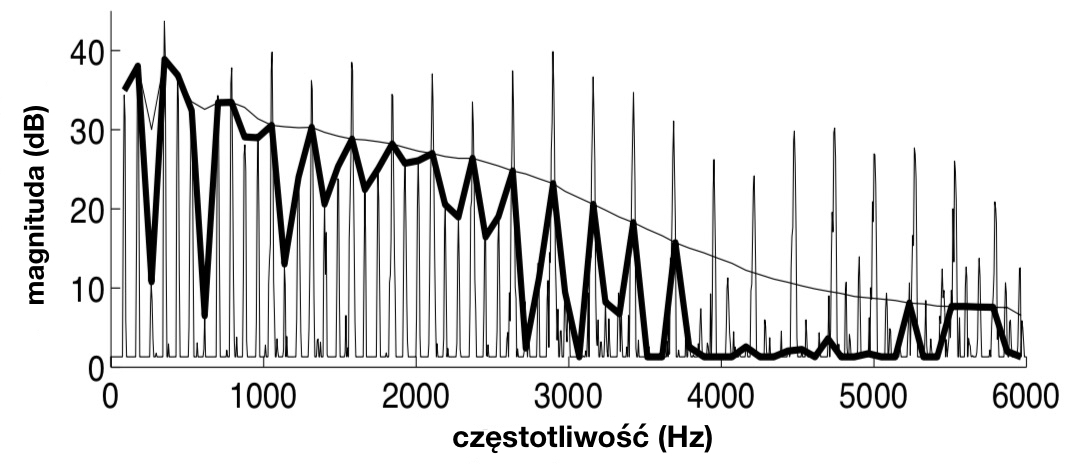
\includegraphics[scale=0.38]{images/spectral_smoothnes_kapuri.jpg}
    \caption{Zobrazowanie zasady gładkości spektrum. Logarytmiczne spektrum mocy zawierające dwa dźwięki. Widmo zostało przefiltrowane przez liftering wysoko przepustowy. Wykres z 
    \cite[3383]{Transcription:Klapuri:MultipitchEstimationAndSeparation}
    %\cite[r. 4]{Transcription:Klapuri:MultipitchEstimationAndSeparation}
    .}
    \label{fig:specSmooth:kapuri}
  \end{center}
\end{figure}

Klapuri kategoryzuje trudności związane z relacjami wysokości dźwięków na dwie grupy:
\begin{itemize}
\item W trakcie usuwania wykrytego dźwięku ze spektrum, harmoniczne innego dźwięku mogą być usunięte, co spowoduje utrudnienie albo nawet uniemożliwienie wykrycia tego dźwięku
\item Dwie lub więcej F0 są ze sobą w takiej relacji, że w widmie pojawia się nieistniejący dźwięk ,,duch''. Dzieje się tak np. gdy dwa F0, o częstotliwościach odpowiednio $2F$ i $3F$ są grane równolegle, harmoniczne obu dźwięków nakładają się z co drugimi i trzecimi harmonicznymi nie granego dźwięku o częstotliwości F0 równej $F$. Tak powstały dźwięk może zostać niewłaściwie wykryty przez algorytmy transkrypcji.
\end{itemize}
Trudności te mają być zminimalizowane poprzez nałożenie funkcji wygadzającej na badane spektrum. Przykład przedstawiony na rysunku \ref{fig:specSmooth:kapuri} obrazuje funkcję wygładzenia (cieńka linia) nałożoną na spektrum podczas badania pierwszego dźwięku, które obrazuje, że co trzeci pik jest wysoko ponad zakładaną krzywą, i to one zostałyby w widmie po odjęciu wygładzonego widma pierwszego dźwięku ze spektrum sygnału. Ten sam mechanizm może pozwolić na wyeliminowanie nieistniejących dźwięków ,,duchów''.

Gładkość spektrum jest założeniem, które jest prawdziwe dla większości przypadków, lecz nie jest to cecha, którą posiadają wszystkie dźwięki. W zależności od źródła wibracji, otoczenia i sposobu w jaki sygnał jest nagrany charakterystyka widma może odbiegać od tej, którą zakłada gładkość spektrum. Silniejsze formanty występujące na wyższych częstotliwościach są cechą wielu instrumentów akustycznych. W celu zminimalizowania błędów spowodowanych założeniem gładkości spektrum powstała kategoria algorytmów bazujących na wyuczonych modelach dźwięków. Zakładają one istnienie modeli dla każdego ze źródeł dźwięków, które mogą występować w analizowanym sygnale, które to są wykrywane w widmie. Problemem w takim podejściu jest ilość potrzebnych danych - w muzyce zachodniej wykorzystywanych jest bardzo dużo różnych instrumentów, z bardzo odległymi od siebie charakterystykami widmowymi. Potrzebne dane treningowe, poprawnie oznaczone według wysokości F0 oraz użytego instrumentu na skale ogólnej analizy popularnej muzyki zachodniej są praktycznie niemożliwe do usystematyzowania. Jednym z ułatwień jest wykorzystanie pojedyńczego nagrania F0 na danym instrumencie i przesuwanie go w wymiarze częstotliwości, aby symulować inne wysokości F0, ale nie jest to niezawodne rozwiązanie, ponieważ wiele instrumentów ma różne charakterystyki widmowe podczas grania różnych częstotliwości fundamentalnych 
\cite[55-68]{Transcription:Quenneville:Thesis}
%\cite[r. 6]{Transcription:Quenneville:Thesis}
.

\subsubsection{Nieharmoniczność} \label{sec:multif0:inh:model}
Wiele algorytmów zaprojektowanych do transkrypcji muzyki bierze pod uwagę problem nieharmoniczności dźwięku. Jak opisuje Klapuri w pracy 
\cite[806-808]{Transcription:Klapuri:MultipleFundamentalFrequencyEstimation}
%\cite[r. 2]{Transcription:Klapuri:MultipleFundamentalFrequencyEstimation}
, fizyczne źródła dźwięków wytwarzają harmoniczne, które nie posiadają dokładnych częstotliwości będącymi wielokrotnościami F0, lecz jedynie oscylują w ich okolicy. Dla przykładu, rozbieżność tą dla instrumentów strunowych można opisać jako:
\begin{equation}\label{eq:inharmonicity:strings}
  f_h = hF \sqrt{1 + (h^2 - 1) \beta}
\end{equation}
gdzie F jest częstotliwością fundamentalną a $\beta$ jest współczynnikiem nieharmoniczności 
\cite[807]{Transcription:Klapuri:MultipleFundamentalFrequencyEstimation}
%\cite[r. 2]{Transcription:Klapuri:MultipleFundamentalFrequencyEstimation}
.

W przytoczonej wcześniej pracy 
\cite[1-10]{Transcription:BayesianHarmonicModels}
%\cite[r. 1-2]{Transcription:BayesianHarmonicModels}
 Davy i Godsill zaproponowali model bayesowski, który bierze pod uwagę nieharmoniczność (nazywaną w tej pracy jako nie-nastrojenie, z ang. \textit{de-tuning}). Opisany w tej pracy jest model zarówno dla sygnałów monofonicznych, jak i dla polifonicznych. Ten drugi zapisany jest jako dyskretne obserwacje $y$ w domenie czasu $t$ w następujący sposób:
\begin{equation}\label{eq:inharmonicity:bayesian}
  y_t = \left\{ \sum_{k=1}^{K}\sum_{m=1}^{M_k}\sum_{i=1}^{I} a_{k,m,i} \phi_{i,t}\cos[(m + \delta_{k,m})\omega_{0,k}t] + b_{k,m,i}\phi_{i,t}\sin[(m + \delta_{k,m})\omega_{0,k}t]\right\} + v_t
\end{equation}
dla $t = 0,1,...,N-1$, gdzie $K$ jest liczbą równolegle granych dźwięków w momencie $t$, $M$ to ilość występujących harmonicznych dla danego dźwięku, $\omega_{0,k}$ to częstotliwość fundamentalna dźwięku $k$, nieharmoniczność przedstawiona jako $\delta = [\delta_1, ..., \delta_K]$, gdzie $\delta_k = [\delta_{k,1}, ..., \delta_{k, M_{k}}]^T$. $I$ jest stałe, znane, i jego celem jest reprezentacja amplitudy jako gładkiej funkcji bazowej $\theta = [a_{1,1,1}, b_{1,1,1}, ..., a_{K, M_{K},I}, b_{K, M_{K},I}]^T$. Można zauważyć podobieństwo do wzoru  \ref{eq:Yeh:signal} przedstawionego przez Yeh'a i Röbel'a. Autorzy \ref{eq:inharmonicity:bayesian} opisują parametr nieharmoniczności jako:
\begin{displayquote}
,,Wektor drobnego de-nastrojenia harmonicznych $\delta$. Jego wartość powinna być bliska zeru i bez relacji względem $\delta$ pozostałych harmonicznych, pomimo tego, że instrument w teorii determinuje rozkład kolejnych harmonicznych. W tym przypadku zakłada się zerową średnią niezależność Gaussa, z wariancją $\sigma_{\delta}^{2}$, ustalony dla małych wartości aby faworyzować małe parametry de-nastrojenia. Rozkład można dodatkowo obciąć tak, aby sąsiednie harmoniczne nie krzyżowały się w domenie częstotliwości'' 
\cite[9]{Transcription:BayesianHarmonicModels}
%\cite[r. 2.4]{Transcription:BayesianHarmonicModels}
(tłumaczenie własne).
\end{displayquote}
\subsubsection{Metoda Pertusa i Iñesta (2008)} \label{sec:pertus1}
Metoda, którą opracowali razem Antonio Pertusa i José M. Iñesta w 2008 roku, nosi nazwę ,,Estymacja wielu częstotliwości fundamentalnych z użyciem gładkości Gaussa'' (tłumaczenie własne) \cite{Transcription:Pertus:Inharmonicity}. Jest to metoda łączona, wykorzystująca okno Gaussa do wygładzenia wyniku. Algorytm ten przetwarza dane przed faktyczną analizą, jak zostało to opisane w sekcji \ref{sec:preProcessing}, wykorzystuje zasadę gładkości spektrum opisaną w sekcji \ref{sec:specSmoothnes} i bierze pod uwagę spektralną nieharmonicznych, której problem opisany był w sekcji \ref{sec:multif0:inh:model}.

Algorytm wykonuje estymacje F0 operując na spektrum kolejnych okien czasowych. Analizowane fragmenty sygnału wejściowego przygotowane są tak, aby miały długość 93 ms (4096 sampli przy częstotliwości samplowania równej 44,1 kHZ) z zastosowaniem funkcji Hanninga jako funkcję okna (opisane w \ref{sec:STFT}) oraz marginesu zer równego trzykrotności długości oryginalnego okna (opisane w \ref{sec:przetwarzanieFFT}). Na tak przygotowanym oknie wykonywane jest STFT (\ref{sec:STFT}), którego wynik ma 16384 spektralnych komponentów, więc każdy z nich ma pasmo szerokości 2.7 Hz (szerokość pasma jest liczona wzorem $h = Fs / N$, gdzie Fs jest częstotliwością próbkowania, a N długością okna).

Dla każdego okna wyniku STFT wykonywane jest przetwarzanie wstępne. Polega ono na odrzuceniu wszystkich wyników, których amplituda jest poniżej wyznaczonego progu $\mu$, i tylko pozostałe brane są pod uwagę. W implementacji tego kroku wprowadzona została modyfikacja, która zakłada że tak odfiltrowane wyniki są tylko pikami. Z tym założeniem, gdy w danym zakresie jest wiele komponentów o amplitudzie wyższej niż $\mu$, zachowywany jest tylko jeden, o najwyższej amplitudzie.

W kolejnym kroku ze spektralnych pików wybierany jest zbiór częstotliwości nazywany ,,kandydatami F0''. Pik jest uznawany za kandydata jeżeli jego częstotliwość jest w zadanym zakresie $[f_{min}, f_{max}]$, oraz posiada on w danym spektrum co najmniej $\eta$ harmonicznych. Pierwszy z warunków obcina grupę analizowanych F0 do jedynie tych, które realnie mogą występować w kompozycji. Badanie skrajnie niskich lub skrajnie wysokich w tonie dźwięków jest niepotrzebne, ponieważ nie są one wykorzystywane w muzyce. Drugie założenie ogranicza grupę kandydatów odrzucając tych, których barwa jest niemożliwa do określenia. Aby wykryć harmoniczne danego F0 sprawdzane jest istnienie pików o częstotliwości będącej wielokrotnością częstotliwości kandydata F0. W celu dostosowania się do nieharmoniczności, badane częstotliwości są w zasięgu ze stałym marginesem $hf_0 \pm f_r$ dla $h = 2, 3, ...$, gdzie $f_0$ jest kandydatem F0. Wybierany jest pik najbliższy faktycznej wielokrotności $f_0$. W przypadku nie znalezienia żadnego piku w danym zakresie, harmoniczna uznawana jest za brakującą. W następnym kroku lista kandydatów sortowana jest względem sumy amplitud ich harmonicznych. Dodatkowych parametrem jest maksymalna liczba kandydatów $F$, na podstawie której odrzucani są nadmiarowi kandydaci o najmniejszej sumie amplitud, aby zwiększyć wydajność tego systemu transkrypcji.

Na podstawie kandydatów generowane są wszystkie możliwe ich kombinacje, a następnie wyliczane dla nich współczynniki ,,istotności'' (z ang. \textit{salience}) oznaczony później jako $S$. Kombinacja, dla której wartość tego współczynnika jest największa jest wybierana, co oznacza, że w danym oknie czasowym wszyscy kandydaci F0 danej kombinacji są obecni w kompozycji. Aby zredukować złożoność obliczeniową tego kroku, generowane są kombinacje z maksymalnie $C$ kandydatami, co przekłada się na założenie maksymalnie $C$ równoległych nut granych w tym samym czasie w analizowanym utworze.

Istotnością kombinacji jest suma współczynnika istotności każdego z jej kandydatów. Jako istotność brane są pod uwagę amplitudy poszczególnych harmonicznych F0 wyliczane na podstawie gładkości ich widm. Dla pojedyńczego kandydata $c$ wyznaczany jest wektor ,,wzoru widmowego'' $p$, który zawiera informacje o amplitudach każdej z harmonicznych kandydata. W literaturze wektor ten powszechnie określany jest jako \textit{HPS}, z angielskiego \textit{hypothetical partial sequences} czyli hipotetyczne częściowe sekwencje (tłumaczenie własne) 
\cite[1118]{Transcription:Yeh:JointEvaluationF0:2}
%\cite[r. IV A]{Transcription:Yeh:JointEvaluationF0:2}
. Na podstawie tych wektorów wywoływany jest iteracyjny algorytm, którego celem jest oznaczenie przynależności każdej harmonicznej do kandydatów występujących w danej kombinacji. Kategoryzuje on harmoniczne na dwie grupy: te, które są w widmie tylko jednego kandydata i te, które występują w widmach kilku kandydatów (i muszą zostać ,,wygładzone'').

Wyliczanie istotności odbywa się dla każdego kandydata osobno, zaczynając od tych z najniższą częstotliwością. Na podstawie danego wzoru widmowego $p_c$ dla kandydata $c$ wszystkie harmoniczne, które występują w więcej niż jednym widmie, są liniowo interpolowane przy użyciu harmonicznych, które nie są dzielone pomiędzy kandydatów. Po tej operacji istnieją dwie możliwości:
\begin{enumerate}
\item interpolowana wartość jest większa lub równa amplitudzie dzielonej harmonicznej. W tym przypadku amplituda uwzględniana przy liczeniu istotności kandydata $c$ dla tej harmonicznej jest brana ze wzoru widmowego $p_c$, natomiast we wszystkich pozostałych wektorach $p$, w których występuje ta harmoniczna, amplituda jej jest zerowana.
\item interpolowana wartość jest mniejsza od amplitudy dzielonej harmonicznej. W tym przypadku interpolowana wartość przypisywana jest do wzoru widmowego $p_c$, a w pozostałych wektorach, w których występuje ta harmoniczna, amplituda jej jest pomniejszana o interpolowaną wartość.
\end{enumerate}
Proces ten ma na celu wygładzenie spektrum dla każdego z kandydatów $c$, zgodnie z zasadą gładkości opisaną w sekcji \ref{sec:specSmoothnes}.

Z tak przygotowanych wzorców widmowych wyliczana jest głośność $l(c)$ dla każdego kandydata $c$ poprzez zsumowanie amplitud z $p_c$.
\begin{equation}\label{eq:inharmonicity:loudness}
  l(c) = \sum_{h=1}^H p_{c,h}
\end{equation}

Wyliczany jest również współczynnik gładkości $\sigma$ dla każdego $c$ z użyciem gładkości Gaussa. Wektor $p_c$ jest filtrowany dolno-przepustowo przy pomocy obciętego znormalizowanego okna Gaussa z trzema komponentami $N_{\sigma = 1.0} = \left\{0,21, 0,58, 0,21\right\}$, które nakłądane jest na wzorzec spektralny danego kandydata tworząc wygładzony wzorzec $\widetilde{p}$. Mając wygładzony HPS, wyliczany jest współczynnik ostrości danego kandydata $s(c)$ jako suma wartości bezwzględnej różnicy wygładzonego i oryginalnego wzorca. Wynik tej operacji normalizowana jest poprzez wyliczenie ilorazu z ilością harmonicznych w wektorze $p_c$:
\begin{equation}\label{eq:inharmonicity:sharpness}
  \overline{s}(c) = \frac{1}{H}\sum_{h=1}^H \left(\left|\widetilde{p}_{c,h} - p_{c,h}\right|\right)
\end{equation}
Tak wyliczony współczynnik ostrości wykorzystuje się do obliczenia współczynnika gładkości $\sigma(c)$, który jest przeciwnością $\overline{s}(c)$:
\begin{equation}\label{eq:inharmonicity:smoothnes}
  \sigma(c) = 1 - \overline{s}(c) 
\end{equation}

Istotność wyliczana jest na podstawie współczynników głośności i gładkości każdego z kandydatów jako
\begin{equation}\label{eq:inharmonicity:salience}
  S = \sum_{c=1}^C\left[l(c)*\sigma(c)\right]^2
\end{equation}
gdzie C to ilość kandydatów danej kombinacji. Kombinacja  odrzucana jest, gdy różnica wartości współczynników głośności pomiędzy dwoma dowolnymi jej kandydatami przekracza ustaloną wartość $\gamma$. Jest to zabezpieczenie przed wyborem kombinacji, w których istnieje grupa kandydatów o zaniedbywalnej głośności. W takim wypadku powinna zostać wybrana inna kombinacja.

W pracy opisującej algorytm autorzy zaproponowali zastosowanie przetwarzania końcowego, które zminimalizuje ilość błędów w transkrypcji 
\cite[106-107]{Transcription:Pertus:Inharmonicity}
%\cite[r. 2]{Transcription:Pertus:Inharmonicity}
. Składa się ono z dwóch operacji:
\begin{enumerate}
  \item założenie znalezienia konkretnej nuty, jeżeli nie była wykryta w danym oknie czasowym, ale była wykryta w poprzednim i następnym oknie
  \item usunięcie bardzo krótkich dźwięków. W pracy zasugerowano minimalną długość sześciu okien (przy założeniach wstępnych 55.68 ms)
\end{enumerate}
Tak przetworzone dane są zapisywane do pliku MIDI na podstawie informacji o początku dźwięku, jego długości oraz wysokości.

\subsubsection{Metoda Pertusa i Iñesta (2012)}\label{sec:petrus2}
Opisana w sekcji \ref{sec:pertus1} metoda do równoległej estymacji F0 w każdym z okien czasowych została po czterech latach rozszerzona na podstawie nowych dokonań w dziedzinie transkrypcji muzyki i opisana przez tych samych badaczy w pracy \cite{Transcription:Pertus:Inharmonicity2}. Założenia metody pozostają bez zmian - dla każdego badanego okna wyliczane są współczynniki istotności w oparciu o kombinacje kandydatów F0, i wybierana jest kombinacja o największym współczynniku $S$. Różnicę od pierwotnej metodologi, jakie narzuca znowelizowany algorytm, składają się z uaktualnia sposób wyliczania istotności o normalizację współczynnika gładkości oraz dodania zaawansowanych technik przetwarzania końcowego dla każdego okna w oparciu o okna sąsiednie. Ogólny schemat działania tej metody jest przedstawiony na rysunku \ref{fig:petrusa_2012_methodology}.

\begin{figure}[ht]
  \begin{center}
    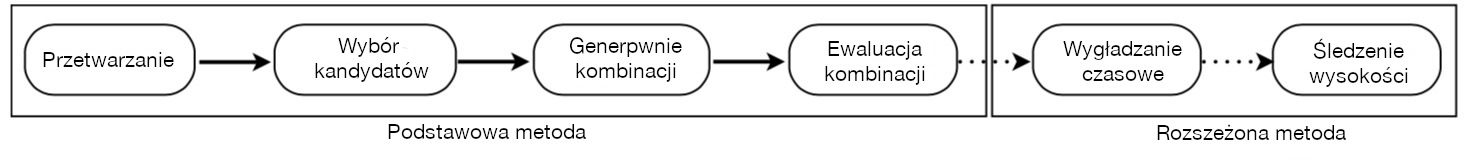
\includegraphics[scale=0.31]{images/Pertusa_2012_methodology.png}
    \caption{Ogólny podgląd metody z podziałem na metodę podstawową opisaną w \cite{Transcription:Pertus:Inharmonicity} i rozszerzoną opisaną w \cite{Transcription:Pertus:Inharmonicity2}. Schemat z \cite[3]{Transcription:Pertus:Inharmonicity2}, tłumaczenie własne.}
    \label{fig:petrusa_2012_methodology}
  \end{center}
\end{figure}

Dla danej kombinacji kandydatów częstotliwości fundamentalnych $c$ wyliczanie parametru wykonywane jest tak samo jak w podstawowej metodzie, tj. zgodnie ze wzorem \ref{eq:inharmonicity:loudness}. Odrzucane są kombinacje, które posiadają kandydata z głośnością poniżej wyznaczanego progu ($l(c) < \eta$), lub takie, w których różnica pomiędzy najcichszym i najgłośniejszym kandydatem jest wystarczająco duża ($l(c) < \gamma L_C$, z $L_C$ będącym głośnością najgłośniejszego kandydata), tak samo jak w metodzie podstawowej.

Istotna zmiana pojawia się podczas liczenia parametru gładkości danego kandydata. Wektor HPS $p_c$ danego kandydata jest poddawany normalizacji poprzez podzielenie jego wartości przez jego maksymalną wartość, skalując go do przedziału $\left<0-1\right>$. Tak znormalizowany HPS jest oznaczany jako $\overline{p}$. Kolejno wzory na wygładzony wektor wzoru widmowego i współczynnik ostrości danej kombinacji są wyliczane z użyciem znormalizowanego HPS:
\begin{equation}\label{eq:inharmonicity2:hpsSmoothed}
  \widetilde{p} = N_{0,1}\ast \overline{p}_c 
\end{equation}
\begin{equation}\label{eq:inharmonicity2:sharpness}
  r(c) = \sum_{h=1}^H\left|\widetilde{p}_{c,h} - \overline{p}_{c,h} \right|
\end{equation}
Współczynnik $r(c)$ w podstawowej wersji jest normalizowany za pomocą podzielenia go przez ilość harmonicznych danego kandydata F0. Normalizacja ta jest rozszerzona w 
\cite[5-6]{Transcription:Pertus:Inharmonicity2} 
%\cite[r. 2.4.2]{Transcription:Pertus:Inharmonicity2} 
tak, aby był niezależny od natężenia:
\begin{equation}\label{eq:inharmonicity2:roughness}
  \widetilde{r}(c) = \frac{r(c)}{H(1 - N_{0, 1}(\overline{x}))}
\end{equation}
Wzór liczenia współczynnika gładkości na podstawie znormalizowanego współczynnika ostrości pozostaje niezmieniony (\ref{eq:inharmonicity:smoothnes}).

Wzór na istotność pojedyńczego kandydata został rozszerzony o parametr $k$, którego zadaniem jest zbalansowanie wkładu gładkości na ten współczynnik:

\begin{equation}\label{eq:inharmonicity2:salience}
S(c) = l(c) * \sigma^k(c)
\end{equation}
Liczenie istotności danej kombinacji jest niezmieniony (\ref{eq:inharmonicity:salience}). W danym oknie wybierana jest kombinacja kandydatów o największym współczynniku $S$. Po ewaluacji każdego okna analizowanego utworu wykonywane jest przetwarzanie końcowe z wykorzystaniem sąsiednich okien, które skłąda się z dwóch etapów: wygładzania czasowego oraz śledzenia wysokości. Wzbogacają one omawianą metodę o informację na temat kontekstu każdego z okien czasowych pozwalając na oszacowanie spójniejszego wyniku.

Wygładzenie czasowe jest procesem przeliczenia istotności każdej z kombinacji w oparciu o sąsiednie okna czasowe. Celem tej operacji jest wybór najbardziej prawdopodobnej kombinacji na przestrzeni $2K + 1$ okien, a nie tylko w kontekście analizowanego odcinka czasowego.

Wszystkie kombinacje poddawane są procesowi kwantyzacji z postaci częstotliwości na notację muzyczną (np. gdy kombinacja składa się z peaków $C_1 = [261 Hz, 416 Hz]$ mapowane jest to na kombinację $C_1' = {C_4, G\sharp_4}$). Na tak przygotowanych kombinacjach liczona jest wygładzona istotność $\widetilde{S}$ z użyciem sąsiadujących okien:
\begin{equation} \label{eq:inharmonicity2:smoothedSalience}
  \widetilde{S}(C_i'(t)) = \sum_{j = t - K}^{t+K}S(C_i'(j))
\end{equation}
gdzie $C_i'(t)$ to kombinacja $i$ po procesie kwantyzacji w czasie $t$. W ogólności, we wszystkich $2K$ oknach wokół okna o indeksie czasowym $t$ wybierane są kombinacje zawierające dokładnie te same nuty, i następnie sumowana jest ich istotność w celu uzyskania nowego wyznacznika, na którego podstawie wyznaczana jest najbardziej prawdopodobna kombinacja:

\begin{equation} \label{eq:inharmonicity2:smoothedSalience:winner}
\widehat{C}'(t) = \arg \max_i \left\{\widetilde{S}(C_i'(t))\right\}
\end{equation}
Tak wybierane kombinacje są bardziej spójne w domenie czasowej, niwelując gwałtowne zmiany wykrytych częstotliwości.

Śledzenia wysokości zaproponowane w pracy 
\cite[7-8]{Transcription:Pertus:Inharmonicity2} 
%\cite[r. 3.2]{Transcription:Pertus:Inharmonicity2} 
jest drugą metodą, która wymusza wybór kombinacji o gładkim przejściu z jednej na drugą w czasie. Metoda ta polega na skonstruowaniu warstwowego, ważonego, ukierunkowanego grafu acyklicznego (wDAG, z ang. \textit{weighted directed acyclic graph}).

Graf $G = \left(V, v_b, E, w, t\right)$ będący warstwowym wDAG składa się ze zbioru wierzchołków $V$, wierzchołka początkowego $v_b$, zbioru krawędzi $E$, funkcji $w$ będącej wagą krawędzi pomiędzy dwoma wierzchołkami w sąsiednich warstwach grafu $w(v_b, v_j)$ oraz funkcji pozycji $t: V \rightarrow \left\{0, 1, 2, ..., T\right\}$. Wierzchołkami są kombinacje kandydatów F0 w danym oknie czasowym, natomiast $t$ dla każdego wierzchołka przyporządkowuje okno czasowe, w którym rozpatrywana jest dana kombinacja. Warstwą nazywane są wszystkie wierzchołki, dla których funkcja $t$ daje ten sam wynik $t(v) = \tau$. W innych słowach, warstwą w grafie jest zbiór kombinacji w jednym oknie czasowym.

Krawędzie prowadzone są ze wszystkich wierzchołków warstwy dla $t(v_i) = \tau$ do wszystkich krawędzi warstwy następnej $t(v_j) = \tau + 1$. Waga krawędzi liczona jest według wzoru:

\begin{equation}\label{eq:inharmonicity2:dwagWeight}
w(v_i, v_j) = \frac{D(v_i, v_j)}{\widetilde{S}(v_j) + 1}
\end{equation}
gdzie $\widetilde{S}$ oznacza istotnością kombinacji warstwy do której prowadzona jest krawędź, liczona według wzoru \ref{eq:inharmonicity2:smoothedSalience}, a $D(v_i, v_j)$ jest współczynnikiem podobieństwa pomiędzy kombinacjami odpowiadającymi wierzchołkom $v_i$ i $v_j$ liczona jako:
\begin{equation}\label{eq:inharmonicity2:dwag:similarity}
D(v_i, v_j) = \sum_{\forall_{C\in v_i, v_j}}\left|\widetilde{l}(v_{i,c}) - \widetilde{l}(v_{j,c}) \right| + \sum_{\forall_{C\in v_i - v_j}}\widetilde{l}(v_{i,c}) + \sum_{\forall_{C\in v_j - v_i}}\widetilde{l}(v_{j,c})
\end{equation}
gdzie $\widetilde{l}(v_{i,c})$ oznacza ogólną głośność kandydata $c$ w kombinacji $i$. Zgodnie z powyższym wzorem \ref{eq:inharmonicity2:dwag:similarity} koszt przejścia pomiędzy wierzchołkami, które mają więcej wspólnych kandydatów będzie mniejsza od tych, które mają więcej rozłącznych kandydatów F0.

W trakcie budowania wDAG w celu zwiększenia wydajność wybieranych jest tylko $M$ najbardziej prawdopodobnych kombinacji dla każdego okna czasowego. Po wygenerowaniu grafu na podstawie wag liczonych wzorem \ref{eq:inharmonicity2:dwagWeight} wyznaczana jest najkrótsza ścieżka przy pomocy algorytmu Dijkstry \cite{Transcription:Dijkstra:Graphs} od pierwszego okna ($t(v) = 0$) do ostatniego ($t(v) = T$). Te wierzchołki, które należą do najkrótszej ścieżki odpowiadają kombinacjom, które są ostatecznie wybierane jako wynik algorytmu.

\subsection{Metody z wykorzystaniem uczenia maszynowego}
Jak było to opisane w sekcji \ref{sec:modelowanieSystemu}, obecnie najbardziej efektywnymi metodami w dziedzinie transkrypcji muzyki są te oparte na NMF oraz na sieciach neuronowych (NN, z ang. \textit{Neural Network}). Te drugie można zaobserwować na szczytach list wyników porównania efektywności modeli transkrypcji, takich jak MIREX (z ang. \textit{The Music Information Retrieval Evaluation eXchange}, framework do formalnej ewaluacji wydajności algorytmów wydobywających informacje muzyczne z sygnałów cyfrowych), już w 2012 
\cite[415-416]{Transcription:Klapuri:ChallengesAndFuture}
%\cite[r. 2.2]{Transcription:Klapuri:ChallengesAndFuture}
. Transkrypcja muzyki jest problemem ściśle powiązanym z zadaniem rozpoznawania wzorców, na którego rozwój w ostatnich latach znaczący wpływ miały metody używające NN 
\cite[26-28]{DBLP:journals/spm/BenetosDDE19}
%\cite[sekcje pt. "NNs for AMT" i "A comparison of NMF and NN models"]{DBLP:journals/spm/BenetosDDE19}
.

%to chyba nie ma znaczenia, więc komentuje. -> W literaturze naukowej jednym z pierwszych wartych uwagi rozwiązań wykorzystujące sieci neuronowe jest \cite[439-440]{Transcription:Marolt:FirstNN}. Użyte zostały tam sieci czasu-opóźnienia (z ang. \textit{time-delay}), które można opisać jako sieci konwolucyjnych ukierunkowanych w czasie, badające wynik banku filtrów gammatone \cite[6]{DBLP:journals/spm/BenetosDDE19}.

W dalszej części tej sekcji zostaną omówione dwa systemy transkrypcji oparte na sieciach neuronowych. Pierwszy z nich będący transkrypcją na poziomie notacji muzycznej \ref{sec:multif0:petrusNetwork}, drugie zaś na poziomie nut \ref{sec:multif0:onsetsAndFrames}, będący do tej pory najefektywniejszym systemem transkrypcji 
\cite[27]{DBLP:journals/spm/BenetosDDE19}
%\cite[sekcja pt. "A comparison of NMF and NN models"]{DBLP:journals/spm/BenetosDDE19}
. W ramach tej pracy nie zostaną opisane dokładne szczegóły dotyczące działania sieci a jedynie pokrótce omówione specyficzne aspekty użytych architektur.


\subsubsection{Holistyczna metoda z użyciem sieci neuronowych}\label{sec:multif0:petrusNetwork}
Praca \cite{Transcription:Pertus:NeuralNetwork} miała na celu zbudowanie architektury zdolnej do transkrypcji A2S (Audio do partytury z ang. \textit{Audio-to-Score}). Jest to rzadkie podejście, wykorzystujące poziom abstrakcji notacji muzycznej. Wiele spośród istniejących algorytmów zakłada transkrypcję do plików MIDI lub podobnych, których struktura opiera się na zapisie rolki pianina, umożliwiając z tego poziomu wygenerować notację muzyczną. Omawiany w tej sekcji algorytm zakłada bezpośredni proces transkrypcji cyfrowego sygnału akustycznego do notacji muzycznej.

Proces określenia partytury ma wiele różnic od tego, którego celem jest wygenerowanie transkrypcji w postaci MIDI. Nawet bezbłędne A2S nie jest w stanie wiernie odzwierciedlić kompozycji muzycznej z sygnału ze względu na ekspresywny charakter wykonania. Kompozycja zapisana w postaci notacji muzycznej może być wykonana na wiele różnych sposobów w zależności od interpretacji. Odwrotna relacja również zachodzi - to samo wykonanie ma różne reprezentacje w postaci partytury. W zależności od przyjętej szczegółowości transkrypcji, różne parametry muzyczne mogą być badane, które w dalszej kolejności przekładają się na symbole muzyczne występujące w partyturze, takie jak oznaczenia tempa, metrum (sygnatura czasowa), klucz, w którym została napisana kompozycja, oznaczenia artykulacji itp.

Algorytm opisywany w \cite{Transcription:Pertus:NeuralNetwork} zakłada pewien stały alfabet notacji muzycznych, za pomocą którego można zdefiniować analizowany utwór. Opisywany A2S przedstawiony jest jako funkcja dziedziny domeny plików dźwiękowych $f : \mathcal{X} \rightarrow \Sigma^{\ast}$, gdzie $\mathcal{X}$ jest domeną plików muzycznych a $ \Sigma $ jest skończonym alfabetem muzycznych symboli.

Model przyjmuje jako dane wejściowe spektralną reprezentację sygnału w czasie uzyskaną poprzez STFT z komponentami rozmieszczonymi logarytmicznie i magnitudą w skali logarytmicznej. Wynikiem jest sekwencja symboli mogąca być zaprezentowana jako zapis nutowy. Symbole określają nuty oraz przerwy z odpowiadającym im czasem trwania, kreski taktowe, łuki pomiędzy nutami oraz fermaty.

Omawiana praca opisuje proces przygotowanych danych treningowych jako nietrywialny ze względu na małą ilość rzetelnych kompozycji w postaci cyfrowych notacji muzycznych. Dokładność obecnej algorytmiki systemów optycznego rozpoznawania muzyki na podstawie zapisu nutowego przez autorów uznawana jest jako niewystarczająca aby użyć jej w celu generowania danych treningowych. Ostatecznie wykorzystana została baza \textit{humdrum-data} dostępna w repozytorium \cite{Transcription:Sapp:Humdrum}. Dane te są w autorskim formacie zaproponowanym w zestawie narzędzi \textit{humdrum}. Format ten jest przeznaczony do ogólnych celów badań nad muzyką. Syntaks \textit{humdrum} nakreśla wzór, którego częścią są inne schematy notacji muzycznej wyższego poziomu, takie jak format \textit{**kern}, na którym oparte są referencyjne dane wykorzystane w opisywanym badaniu. Składnia \textit{**kern} jest szczególnie odpowiednia do tego modelu, ponieważ zaprojektowana jest ona do kodowania alfabetu muzycznego muzyki zachodniej.

Zadanie A2S zadeklarowane jest jako pozyskanie najprawdopodobniejszej sekwencji symboli muzycznych występującej w kompozycji w pliku audio $x \in \mathcal{X}$:

\begin{equation}
\widehat{s} = \arg \max_{s \in \Sigma^{\ast}} P (s | x)
\end{equation}

Podejście holistyczne do rozwiązania zakłada użycie konwolucyjnej rekurencyjnej sieci neuronowej (CRNN, z ang. \textit{Convolutional Recurrent Neural Network}). Architektura CRNN składa się z bloku warstw konwolucyjnych oraz bloku warstw rekurencyjnych. Ten pierwszy odpowiedzialny jest za wydobywanie cech z sygnału wejściowego, drugi zaś odpowiada za wykrywanie cech w kontekście sekwencyjnym. 

Przy $W$ będącym długością sygnału wejściowego (w ilości okien czasowych) długość wektora cech będzie równa $L = \gamma W$, gdzie $\gamma \leqslant 1$, co jest długością aktywacji ostatniej warstwy bloku konwolucyjnego. Wynik ostatniej warstwy konwolucyjnej jest używany jako wejście do bloku warstw rekurencyjnych, którego aktywacja ostatniej warstwy jest estymacją danego okna:
\begin{equation}
  P(\sigma | x, j), 1 \leqslant l \leqslant L, \sigma \in \Sigma 
\end{equation}
Dekodowanie odbywa się poprzez wybranie najbardziej prawdopodobnego symbolu dla każdego wektora cech danego bloku rekurencyjnego, a następnie wyniki są ze sobą łączone i usuwane są symbole puste 
\cite[2-5]{Transcription:Pertus:NeuralNetwork}
%\cite[r. 2-3]{Transcription:Pertus:NeuralNetwork}
.


\begin{figure}[ht]
  \begin{center}
    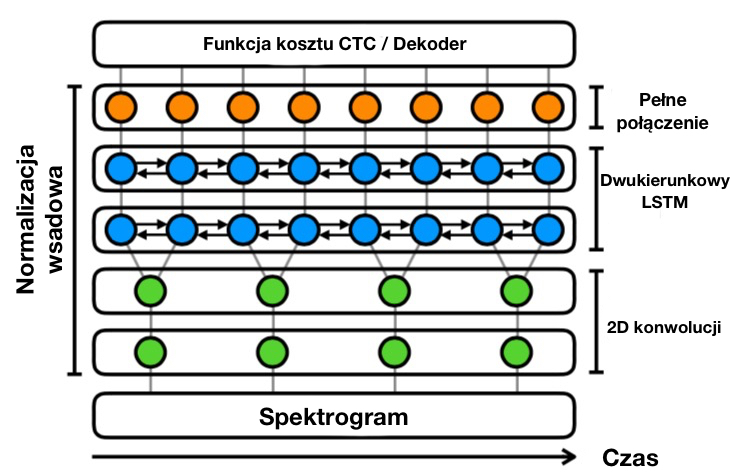
\includegraphics[scale=0.5]{images/holisticNetworkArchitecture.jpg}
    \caption{Architektura sieci neuronowej zastosowanej w pracy  \cite{Transcription:Pertus:NeuralNetwork}. Diagram z 
    \cite[5]{Transcription:Pertus:NeuralNetwork}
    %\cite[r. 3]{Transcription:Pertus:NeuralNetwork}
    , tłumaczenie własne.}
    \label{fig:holisticNetworkArchitecture}
  \end{center}
\end{figure}

Architektura zaprezentowana w omawianej pracy przedstawiona jest na schemacie w \ref{fig:holisticNetworkArchitecture}. Pierwsze dwie warstwy konwolucyjne nakładają 16 filtrów o wymiarach 3 x 3 z krokiem równym 2 na osi częstotliwości. Kolejne dwie warstwy są blokiem rekurencyjnym, w którego skład wchodzą dwukierunkowe sieci z długotrwałą pamięcią krótkoterminową (LSTM, z ang. \textit{Long Short-Term Memory}), każda z nich z 1024 ukrytymi jednostkami. W celu uniknięcia nadmiernego dopasowania dodane są sieci normalizacji wsadowej (ang. \textit{Batch Normalization}) pomiędzy każdą warstwą z wyjątkiem pierwszej i ostatniej, warstwy \textit{dropout} po każdej warstwie konwolucyjnej oraz ostatniej warstwie rekurencyjnej, które przepuszczają tylko fragment danych. Szczegółowy opis użytych parametrów w zależności od danych testowych jest zawarty w omawianej pracy.

%%Pytanie czy dodać wyniki, które są opisane w tej pracy, albo jakąś konkluzje jeszcze tutaj


\subsubsection{Onsets and Frames}\label{sec:multif0:onsetsAndFrames}
Użycie sieci neuronowych do modelowania systemu transkrypcji występuje w literaturze naukowej już od dłuższego czasu. Wyniki tych architektur nie były wyraźnie wyższe od równolegle wynajdywanych sposobów. W ostatnich latach, w ramach projektu Magenta \cite{Transcription:Magenta} powstał system transkrypcji o nazwie \textit{Onsets And Frames} (początki dźwięków i okna, tłumaczenie własne), który, według ewaluacji przedstawionej w dedykowanej pracy naukowej \cite{Transcription:Hawthorne:OnsetsAndFrames}, osiąga rekordowe rezultaty w dokładności wyników.

Projekt Magenta ma na celu wytworzenie algorytmiki i oprogramowania, które ma być narzędziem w rękach artystów. Ma to na celu udowodnienie, że uczenie maszynowe może być pomocne w procesie artystycznie twórczym. Rozwiązania są \textit{open source}, ułatwiając tym samym do nich dostęp. Douglas Eck, członek zespołu pracującego nad Magenta zapewnia, że projekt ten ma na celu dać źródło inspiracji artystom, a nie szukać sposobów ich zastąpienia przez komputery. System transkrypcji, który został opracowany w ramach tego projektu, jest nie tylko docelowym produktem tej koncepcji, ale też narzędziem pozwalającym ewaluować i zasilać danymi inne badane przez Magenta architektury.

Głównym założeniem, które odróżnia Onsets and Frames od innych systemów transkrypcji bazujących na sieciach neuronowych, jest rozłożenie zadania na dwa problemy: wykrywanie początku nuty oraz wykrywanie aktywności nut w oknie. Oba pod\-zadania mają osobne dedykowane sieci. Nuta jest uznawana za obecną wtedy, i tylko wtedy, gdy zostanie dla niej wykryty początek oraz aktywność.

Dane wejściowe są w postaci spektrogramów w skali melowej i logarytmie amplitudy, z 229 logarytmicznie rozmieszczonymi w domenie częstotliwości komponentami, oknem długości 2048 sampli i odstępami pomiędzy oknami długości 2048. Dane równolegle zasilają obie sieci. Wynik detektora początków nut jest dostarczany do sieci aktywacji nuty, dając jej łącznie dwie informacje wejściowe - czy  początek nuty został wykryty oraz spektrogram sygnału.

Detektor początku nuty składa się z modelu akustycznego (jego architektura opisana jest w 
\cite[1-3]{Transcription:Kelz:AcousticModel}
%\cite[r. 1-2]{Transcription:Kelz:AcousticModel}
) połączonego z dwukierunkowym LSTM z 128 jednostkami dla każdego kierunku, który połączony jest z warstwą sigmoidalną, która ma 88 wyjść. Liczba wyników jest równa ilości klawiszy na pełnowymiarowym pianinie. Wykrywacz aktywności nuty zbudowany jest z modelu akustycznego połączonego z sigmoidalną warstwą, analogiczną do tej w detektorze. Jej wynik jest łączony z wynikiem detektora początku nuty jako wejście do dwukierunkowego LSTM z 128 jednostkami dla każdego kierunku. Po tym występuje kolejna warstwa sigmoidalna z analogicznymi do poprzednich parametrami, której wynik po nałożeniu progu 0.5 jest interpretowany jako predykcja danego okna. Architektura ta jest przedstawiona na rysunku \ref{fig:onsetsAndFramesArch}
\begin{figure}[h]
  \begin{center}
    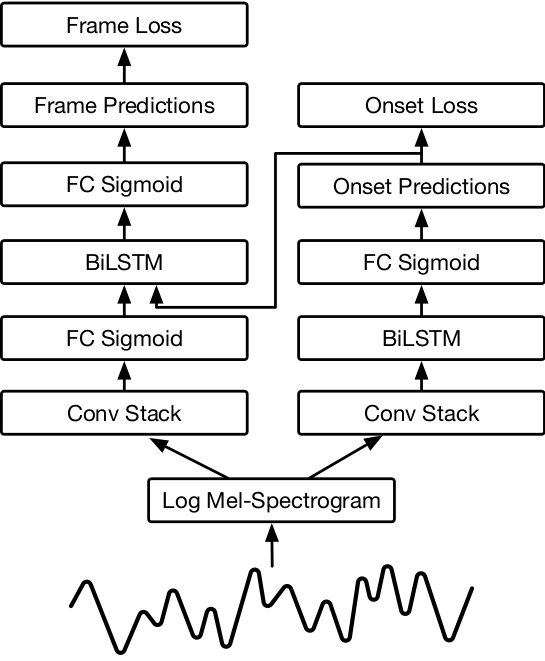
\includegraphics[scale=0.8]{images/architekturaSieciOnesetsFrames.png}
    \caption{Diagram przedstawiający architekturę modelu Onesets and Frames. Diagram z \cite{Transcription:OnsetsAndFrames:Blog}, tłumaczenie własne.}
    \label{fig:onsetsAndFramesArch}
  \end{center}
\end{figure}

Metoda Onsets and Frames wprowadziła detekcje dynamiki, która nie została rozpatrzona przez żaden z istniejących wcześniej modeli. Model zbudowany jest analogicznie, ale nie jest połączony z architekturą opisaną powyżej. Etykiety dynamiki są generowane przez podzielenie wszystkich dynamik przez maksymalną obecną w danym fragmencie. Najmniejsza dynamika jest wyznaczana jako $\frac{v_{min}}{v_{max}}$. Wynik jest przycinany do zakresu $\left[0,1\right]$ a następnie przekształcany do parametru \textit{velocity} w MIDI mapowaniem:
\begin{equation}
  v_{midi} = 80 v_{predicted} + 10
\end{equation}

Opisywana praca została zaktualizowana, co zostało opisane w 
\cite[3-5]{Transcription:Cheng:OnsetsAndFramesNovelization}
%\cite[r. 3]{Transcription:Cheng:OnsetsAndFramesNovelization}
. Pierwotnie, model trenowany i ewaluowany był przy użyciu bazy MAPS \cite{Transcription:OnsetsAndFrames:MAPS}. Na czas powstawania pierwotnej wersji rozwiązania była ona najbardziej odpowiednia biorąc pod uwagę ilość i jakość zawartych w niej danych. W nowszej wersji została ona zamieniona na bazę MAESTRO (z ang. \textit{MIDI and Audio Edited for Synchronous TRacks and Organization}) przygotowaną w ramach opisywanej pracy. MAESTRO zawiera ponad 172.3 godziny sparowanych plików audio z MIDI, co jest trzykrotnie większą ilością danych od bazy MAPS. Zawarte pliki audio są nagraniami wystąpienia pianisty na fortepianie akustycznym Yamaha Disklavier. Nuty w MIDI nakładają się tymi z plików audio z dokładnością do około 3 milisekund. Dzielenie danych na treningowe, walidacyjne i testowe jest wykonane w taki sposób, że ta sama kompozycja, nawet jeżeli wykonana przez różnych artystów, nie występuje w więcej niz jednej grupie. Zasada ta wprowadzona jest w celu uniknięcia efektu nadmiernego dopasowania(z ang. \textit{overfittingu}, tłumaczenie własne) \cite{Transcription:Curtis:MAESTRO}.

Poza użyciem innej bazy, zmiany do Onsets and Frames zaproponowane w 
\cite[3-5]{Transcription:Cheng:OnsetsAndFramesNovelization} 
%\cite[r. 3]{Transcription:Cheng:OnsetsAndFramesNovelization} 
zakładają dodanie detekcji offsetu, która zasila detektor aktywności nut, choć nie jest bezpośrednio używana w dekodowaniu. Zaproponowana jest również zmiana dwukierunkowych warstw LSTM z 128 do 256 jednostek, zmieniając ilość filtrów w warstwie konwolucyjnej z 32/32/64 na 48/48/96, zwiększając tym samym warstwy sigmoidalne. Zmodyfikowane zostały również przejścia pomiędzy podsieciami. Argumentowane są tym, że dla większych baz efektywność rośnie przy większym i prostszym modelu. 

Dodatkowo zaproponowana została metoda augmentacji sygnału wejściowego, która polegać ma na modyfikacji każdego z danych wejściowych o pewną modulację audio (np. przesunięcie częstotliwości, dodanie szumu, zastosowanie equalizera). Zmiana ta pozytywnie wpływa na jakość modelu trenowanego bazą MAPS, jednak w przypadku bazy MAESTRO odnotowany został minimalny spadek w dokładności wyniku. 

\newpage

\section{Implementacja}\label{sec:impl}
Ten rozdział poświęcony jest opisaniu implementacji algorytmów transkrypcji z rozdziałów \ref{sec:f0} i \ref{sec:MultiPitch}, które są częścią projektu powstałego w ramach tej pracy magisterskiej. Kod napisany został w skryptowym języku Python w wersji 3.7.4, który wydawał się najodpowiedniejszy do tego typu zadania ze względu na dostępne biblioteki dedykowane do matematycznych problemów (jak \textit{numpy} czy \textit{scipy}). Szczegółowa lista użytych rozwiązań dostępna jest w pliku README.md dostępnym w głównym katalogu projektu.

Wszystkie z funkcji operujących na danych audio opisanych poniżej zakładają pliki  o rozszerzeniu \textit{.wav} z kodowaniem PCM z 16 lub 32 bitami na sampel. Sygnały, które są dwukanałowe (stereo audio) zostają przed analizą ,,spłaszczone'' do jednego kanału poprzez przemnożenie każdego z nich przez $\frac{1}{2}$ oraz scalenie ich razem poprzez dodanie każdej z wartości. Dane przed analizą są znormalizowane poprzez skalowanie danych do zakresu $\left[0, 1\right]$.

Każda z funkcji implementujących algorytmy transkrypcji muzyki przyjmuje cztery bazowe argumenty odpowiadające danym wejściowym i sposobie ich fragmentacji na okna czasowe:
\begin{itemize}
  \item \textit{data} - znormalizowane dane pobrane z pliku dźwiękowego
  \item \textit{frameWidth} - długość okna w samplach
  \item \textit{sampleRate} - częstotliwość próbkowania
  \item \textit{spacing} - odstęp pomiędzy kolejnymi oknami danych
\end{itemize}

\begin{lstlisting}[language=Python, caption={Przykład pętli po danych wejściowych z uwzględnieniem okna czasowego}, captionpos=b, label={code:iter}]
  for i in range(0, int(math.ceil((len(data) - frameWidth) / spacing))):
    frame = data[i*spacing:i*spacing+frameWidth] * hann
    frame = np.concatenate((frame, zeroPadding))
    frameComplex = fft(frame)
\end{lstlisting}

Sposób iterowania pomiędzy kolejnymi oknami jest również identyczny dla każdej z implementacji i jest przedstawiony na listingu \ref{code:iter}. W lini 2 listingu na konkretne okno danych nakładana jest funkcja okna (w tym przypadku okno Hanna). W przypadku algorytmów operujących na spektrum, do okna dodawana jest odpowiednia ilość zer (linia 3) jako margines zer, i dopiero na tak przygotowanych danych wykonywana jest transformata (linia 4).

Zaimplementowany został również prosty mechanizm porównujący pliki MIDI. Jego celem jest porównanie wyników zaimplementowanych algorytmów w celu ich ewaluacji, co zostało opisane w sekcji \ref{sec:impl:midiCompare}. Wyniki ewaluacji przeprowadzonej na zaproponowanej implementacji opisane są następnie w rozdziale \ref{sec:ewal}. Algorytmy wykrywające F0 w monofonicznym sygnale oryginalnie nie posiadają metodyki przedstawiania wyniku jako plik MIDI. Na potrzeby tej pracy przedstawienie wyniku w postaci MIDI zostało zaimplementowane, czego opis można znaleźć w sekcji \ref{sec:impl:midiGen}.

Poza algorytmami w ramach tej pracy magisterskiej zaimplementowany został również graficzny interfejs (GUI, z ang. \textit{Graphical User Interface}) w postaci aplikacji webowej z dedykowanym serwerem lokalnym napisanym w Python, za pomocą którego można łatwo przetestować działanie zaimplementowanych metod. Krótki opis tego rozwiązania znajduje się w tym rozdziale w sekcji \ref{sec:impl:gui}.

\subsection{Autokorelacja}\label{sec:impl:alg:ac}
Funkcja autokorelacji (\ref{sec:f0:ac}) jest jedynym z zaimplementowanych algorytmów, który operuje na nieprzetworzonym sygnale w domenie czasu. Dodatkowymi parametrami (poza tymi związanymi z parametrami danych i długością okna) są częstotliwości maksymalna i minimalna (jak widać na listingu \ref{code:minMaxLag}), jakie są w zakresie analizy. Na ich podstawie wyznaczane są minimalne i maksymalne przesunięciem, które w dalszej części ograniczają zakres, na którym operuje funkcja autokorelacji, co widać na listingu \ref{code:ac}.
\begin{lstlisting}[ language=Python, caption={Wyliczanie maksymalnego i minimalnego przesunięcia funkcji autokorelacji}, captionpos=b, label={code:minMaxLag}]
  minLag = int(floor(sampleRate / fqMax))
  maxLag = int(ceil(sampleRate / fqMin))
\end{lstlisting}

\begin{lstlisting}[language=Python, caption={Funkcja autokorelacji}, captionpos=b, label={code:ac}]
n = len(data)
result = list(np.zeros(min_lag))
for lag in range(min_lag, max_lag):
  sumarray = np.zeros(n+lag)
  sumarray[:n] = data
  sumarray[:n-lag] *= data[lag:]
  sum = np.sum(sumarray[:n-lag])
  result.append(float(sum/(n-lag)))
return result
\end{lstlisting}

Funkcja autokorelacji wyliczana jest dla każdego okna czasowego. Zwraca ona wektor długości $minLag - maxLag$ wartości korelacji danych wejściowych z danymi przesuniętymi o $lag$ sampli w prawo. Dla danego okna jako estymację F0 wybierane jest to przesunięcie, które ma najwyższy wynik. Implementacja znajduje się w projekcie w pliku \textit{server/transcription/ac.py}.

\subsection{Cepstrum}\label{sec:impl:alg:ceps}
Cepstrum (\ref{sec:f0:ceps}) w projekcie używany jest w dwóch celach - jako trzon metody do estymacji F0, jak i do filtrowania sygnału w domenie quefrency. Z tego powodu implementacja funkcjonalności została wyniesiona do pomocniczego pliku \textit{utils/cepstrumUtils}. Funkcja \textit{real\_cepst\_from\_signal} przyjmuje okno danych, na którym wyliczane jest cepstrum mocy według wzoru \ref{eq:ceps1} co przedstawione jest na listingu \ref{code:cepsUtil}.

\begin{lstlisting}[language=Python, caption={Wyliczanie cepstrum mocy}, captionpos=b, label={code:cepsUtil}]
  spectrum = fft(data)
  logSp = np.log(np.abs(spectrum))
  ceps = np.abs(ifft(logSp)) ** 2
  return ceps, logSp, spectrum
\end{lstlisting}

Estymacja F0 dla każdego z okien czasowych polega na transformacji danych do cepstrum oraz znalezienie komponentu cepstralnego o największej wartości. Podzielenie quefrency wyznaczonego komponentu przez częstotliwość próbkowania daje w wyniku częstotliwość F0. Pod uwagę branych jest jedynie $n / 2$ pierwszych elementów cepstrum, gdzie $n$ jest ilością danych wejściowych łącznie z marginesem zer (ze względu na symetryczny charakter wyniku cepstrum). Pierwsze elementy wyniku cepstrum nie są brane pod uwagę przy szukaniu maksymalnego komponentu ze względu na znaczne zwiększenie błędności wyniku (pierwsze komponenty cepstralne symbolizują podobieństwo sygnału do samego siebie, analogicznie do autokorelacji), co zostało w implementacji zrobione poprzez wyzerowanie wartości pierwszych 14 elementów wektora cepstrum (linia $4$ listingu \ref{code:cepsF0Cpu}). 

\begin{lstlisting}[language=Python, caption={Estymacja F0 przy pomocy cepstrum}, captionpos=b, label={code:cepsF0Cpu}]
  cepst, logSp, spectr = real_cepst_from_signal(frame)
  fftLen = int(np.floor(len(spectr)/2))
  cepst = cepst[:fftLen//2]
  cepst[0:14] = np.zeros(14)
  cepstra.append(cepst)
  maxperiod = np.argmax(cepst)
  bestFq.append(sampleRate/maxperiod)
\end{lstlisting}

W ramach tej pracy magisterskiej została zaimplementowana wersja analizy cepstralnej przy użyciu karty graficznej GPU (z ang. \textit{graphics processing unit}). Zaimplementowane rozwiązanie zakłada dostęp do API CUDA, z którego korzysta użyta biblioteka dająca dostęp do wywoływania poleceń GPU z poziomu kodu napisanego w języku python. Szczegóły karty jak i stopień uzyskanego przyspieszenia opisane są w rozdziale \ref{sec:ewal}.

Rozwiązanie GPU znajduje się w pliku \textit{server/utils/cepsUtilsGpu.py} w postaci klasy \textit{CepsUtilsGpu} implementującej interfejs biblioteki \textit{reikna} pozwalający na tworzenie planu obliczeń na GPU. Plan ten przyjmuje argumenty w postaci znormalizowanych danych audio, długości okna, długości marginesu zer oraz odległości pomiędzy oknami. Dane poprzez transformację dostosowywane są do formatu wejścia funkcji FFT dostępnej w bibliotece \textit{reikna}. Cały proces, przedstawiony na listingu \ref{code:cepsF0Gpu}, można opisać w następujący sposób:
\begin{enumerate}
  \item dane sygnału wejściowego (\textit{flat\_input}) przekształcane są do tablicy dwuwymiarowej \textit{unwindowed\_input} transformacją \textit{rolling\_frame} tak, że długości wierszy są równe długości ustalonego okna czasowego z długością marginesu zer. Dane składowane są po kolei z uwzględnieniem marginesu zer i odległości pomiędzy oknami;
  \item tablica \textit{unwindowed\_input} przekształcana jest do \textit{input\_real} transformacją \textit{hanning\_window}, która nakłada funkcję Hanna do każdego z wierszy danych wejściowych;
  \item dlatego, że do użytej implementacji FFT wymagane jest podanie danych o typie zespolonym, użyta została transformacja \textit{combine\_complex}, która przyjmuje dwa parametry - dane rzeczywiste, którymi są przygotowana tablica \textit{input\_real} oraz dane urojone, które są wygenerowanie za pomocą funkcji \textit{broadcast\_const} i mają postać tablicy zer takich samych wymiarów jak \textit{input\_real};
  \item na tak przygotowanych danych wykonywana jest funkcja FFT, po której stosowana jest transformacja \textit{log\_pow} dająca w wyniku \textit{log\_pow} będące tablicą spektrum logarytmów mocy;
  \item funkcja IFFT (odwrotność FFT) wywoływana jest na wyniku kolejnej transformacji \textit{combine\_complex}, której danymi wejściowymi rzeczywistymi jest tablica \textit{log\_pow} a urojonymi jest tablica generowana analogicznie do tej, przygotowanej w pkt. 3;
  \item wynik IFFT przekształcany jest transformacją \textit{crop\_frequencies\_ceps}, która zeruje pierwszych 10 wartości (analogicznie do \ref{code:cepsF0Cpu}) oraz wycina elementy przekraczające częstotliwość Nyquista;
  \item wynik \textit{crop\_frequencies\_ceps} jest transponowany i zwracany jako wynik.
\end{enumerate}

\begin{lstlisting}[float, language=Python, caption={Proces wyliczania cepstrum przy użyciu GPU}, captionpos=b, label={code:cepsF0Gpu}]
  fft = FFT(fft_arr, axes=(1,))
  fft.parameter.input.connect(
      to_complex_trf, to_complex_trf.output,
      input_real=to_complex_trf.real, input_imag=to_complex_trf.imag)
  fft.parameter.input_imag.connect(broadcast_zero_trf, broadcast_zero_trf.output)
  fft.parameter.input_real.connect(window_trf, window_trf.output,
  unwindowed_input=window_trf.input)
  fft.parameter.unwindowed_input.connect(
      rolling_frame_trf, rolling_frame_trf.output, flat_input=rolling_frame_trf.input)
  fft.parameter.output.connect(
      log_pow_trf, log_pow_trf.input, log_pow=log_pow_trf.output)
  ifft = FFT(Type(complex_dtype, fft.parameter.log_pow.shape), axes=(1,))
  ifft.parameter.input.connect(
      to_complex_trf, to_complex_trf.output,
      input_real=to_complex_trf.real, input_imag=to_complex_trf.imag)
  ifft.parameter.input_imag.connect(broadcast_zero_trf, broadcast_zero_trf.output)
  crop_trf = crop_frequencies_ceps(ifft.parameter.output)
  ifft.parameter.output.connect(
      crop_trf, crop_trf.input, cropped_amplitude=crop_trf.output)
\end{lstlisting}

\subsection{ACLOS}\label{sec:impl:alg:aclos}
Trzonem metody ACLOS (\ref{sec:f0:aclos}) jest funkcja autokorelacji w domenie częstotliwości, której implementacja jest bardzo podobna do tej w domenie czasu (\ref{sec:impl:alg:ac}). Wyróżniającymi się elementami tego algorytmu są użycie lifteringu na sygnale oraz wykorzystanie interpolacji do zwiększenia dokładności wyniku.   

Filtrowanie w domenie quefrency odbywa się dla każdego okna czasowego, po przekształceniu do nałożeniu funkcji okna oraz przekształceniu do postaci spektrum mocy. Widmo przekształcane jest do cepstrum przy pomocy IFFT, po czym wykonywane jest na nim filtrowanie. Proces ten przedstawiony jest na listingu \ref{code:liftering}. Poza danymi wejściowymi jako argumenty funkcja \textit{lifterOnCeps} przyjmuje typ lifteringu \textit{lifterType} (którym może być funkcja sinusoidalna, trójkątna lub prostokątna) oraz mnożnik \textit{coefficient}.

Estymacja F0 przyjmuje interpolacje sześcienną wyniku funkcji autokorelacji. Na jej podstawie wyznaczana jest częstotliwość z najlepszym wynikiem, co przedstawione jest na listingu \ref{code:bestFqInterpolate}. Zmienna \textit{fftToFq} jest tablicą z wartościami równymi częstotliwości dla kolejnych indeksów wyniku FFT dla danej rozdzielczości. Maksymalny błąd w domenie częstotliwości wiąże się z rozdzielczością wykonywanego FFT i jest równy $\frac{fs}{NFFT}$, gdzie $fs$ jest częstotliwością próbkowania, a $NFFT$ to ustalona długość okna. 

\begin{lstlisting}[float, language=Python, caption={Filtrowanie w domenie quefrency}, captionpos=b, label={code:liftering}]
  k = np.arange(len(ceps))
  h = (coefficient/2.)
  def f(lifterType):
      lift = {
          LifterType.sine: 1 + h * np.sin(np.pi*k/coefficient),
          LifterType.triangle: 1 + h * (k - 1) / (coefficient - 1),
          LifterType.rectangle: np.ones(len(ceps))
      }[lifterType]
      return lift

  lift = f(lifterType)
  return ceps * lift
\end{lstlisting}

\begin{lstlisting}[float, language=Python, caption={Wyznaczanie F0 w ACLOS}, captionpos=b, label={code:bestFqInterpolate}]
  interp_x = np.linspace(0, dataLen-1, num=dataLen*interpolMultiplier)
  argmax = np.argmax(interpolatedAutocorrelation(interp_x))
  correlationArgMax = int(np.round(argmax / interpolMultiplier))
  delta = argmax - (correlationArgMax * interpolMultiplier)
  bestFq = fftToFq[correlationArgMax] + (fqMaxError * delta / interpolMultiplier)
  return bestFq
\end{lstlisting}

\subsection{Metoda Pertusa i Iñesta (2008)}\label{sec:impl:alg:specSmoothnes}
Metody opisane w sekcjach \ref{sec:pertus1} oraz \ref{sec:petrus2} w dużej części się pokrywają, dlatego też implementacja obu metod znajduje się w funkcji \textit{harmonicAndSmoothnessBasedTranscription} w pliku \textit{server/transcription/jointMethodByPertusAndInesta.py}. W przypadku, gdy argument \textit{newAlgorithmVersion} ustawiony jest na wartość \textit{False}, zostanie wykonana metoda zgodna z opisem pracy z 2008 roku \cite{Transcription:Pertus:Inharmonicity}, którego implementacja opisana jest w tej sekcji. W przeciwnym wypadku zostanie wykonana znowelizowana wersja algorytmu z 2012 roku (\cite{Transcription:Pertus:Inharmonicity2}). Trzon metody zaprezentowany jest na listingu \ref{code:coreMethodPetrusa1}.

W pierwszej kolejności wywoływana jest funkcja \textit{coreMethod}, której zadaniem jest przetworzenie sygnału do postaci nut, na którym następnie wykonywane jest przetwarzanie końcowe. Z każdego spektrum okna czasowego po nałożeniu lifteringu wydobywane są wartości (piki) o amplitudach powyżej zadanego progu i na ich podstawie wyznaczani są kandydaci do F0. Zbiór wyznaczonych częstotliwości pomniejszany jest o te, które nie mają wystarczającej ilości harmonicznych w tablicy pików. Liczba kandydatów następnie jest posortowana względem amplitud i odrzucone zostają wszystkie przekraczające indeks \textit{maxCandidates} zmniejszając tym samym ilość kombinacji w przypadku dużej liczby kandydatów.

Kolejnym krokiem jest wyznaczenie wszystkich możliwych kombinacji i wyliczenie istotności każdej z nich. Funkcja obliczająca istotność tworzy kopie tablicy pików i tablicy wszystkich wzorów spektralnych a następnie iteruje po wszystkich kandydatach danej kombinacji:
\begin{enumerate}
  \item kopia pików i wzorów spektralnych zostają wygładzone w oparciu o spektrum danego kandydata funkcją \textit{smoothenPattern} zgodnie z metodą opisaną w \ref{sec:pertus1};
  \item wyliczane zostają głośność jako suma amplitud oraz gładkość danego wzoru spektralnego kandydata F0.
\end{enumerate}
W danym oknie czasowym wybierana jest kombinacja o największej sumie istotności harmonicznych. Lista częstotliwości kandydatów F0 wygranej kombinacji transformowana jest na tablicę, której indeksy oznaczają numery nut MIDI a wartościami jest parametr dynamiki, za którego brana jest średnia amplituda F0 wraz z harmonicznymi.

Przetwarzanie końcowe zaimplementowane w funkcji \textit{postProcessMidiNotes} i wylicza ono dynamikę na podstawie wcześniej nadanej wartości z amplitudy i generuje bardziej ,,spójną'' rolkę pianina, odrzucając zbyt krótkie nuty i łącząc w całość nuty, które były wykryte w oknie o indeksie $n-1$ oraz $n+1$, ale nie były wykryte w oknie o indeksie $n$. Implementacja pozwala na zdefiniowanie ilości sąsiadujących nut branych pod uwagę podczas tego procesu.

\begin{lstlisting}[language=Python, caption={Trzon algorytmu Pertusa i Iñesta (2008)}, captionpos=b, label={code:coreMethodPetrusa1}, numbers=none]
  peaks, candidate = getPeaksAndCandidates(countPowerFftWindow(i))
  hypotheses, amplitudeSum, patterns, ownerships =
    getCandidatesThatHaveEnoughHarmonics(candidate, peaks)
  if(len(hypotheses) == 0):
    resNotes.append({})
    continue
  sortedByFq = getMaxCandidatesByPower(amplitudeSum, hypotheses)
  possibleCombinations = []
  for num_pitches in range(1, min(maxParallelNotes, len(sortedByFq)) + 1):
    for combo in combinations(sortedByFq, num_pitches):
      possibleCombinations.append(combo)
  allSaliences = []
  allMidiNotes = []
  for combination in possibleCombinations:
    combinationSalience = countCombinationSalience(
        combination, patterns, peaks, ownerships)
    allSaliences.append(combinationSalience)
    midiNotes = {}
    for fftFq in combination:
      fq = fft_to_hz_array[fftFq]
      midiNotes[hz_to_midi(fq)] = (amplitudeSum[fftFq] / len(patterns[fftFq]))
    allMidiNotes.append(midiNotes)
  resNotes.append(allMidiNotes[np.argmax(allSaliences)])
\end{lstlisting}

\subsection{Metoda Pertusa i Iñesta (2012)}\label{sec:impl:alg:specSmoothnes:improved}
Gdy funkcja \textit{harmonicAndSmoothnessBasedTranscription} zostanie wywołana z argumentem $newAlgorithmVersion = True$ wykonana zostanie metoda z usprawnieniami opisanymi w sekcji \ref{sec:petrus2} i pracy naukowej \cite{Transcription:Pertus:Inharmonicity2}. Implementacja różni się od tej opisanej w \ref{sec:impl:alg:specSmoothnes} sposobem wyliczania istotności kombinacji oraz przetwarzaniem końcowym.  

Proces wyliczania istotności dla danego kandydata F0 zgodnie z opisem z \cite{Transcription:Pertus:Inharmonicity2} jest przedstawiony na listingu \ref{code:petrusIstotnosc}. Wynikiem trzonu algorytmu, w przeciwieństwie do wersji z 2008 roku, jest lista nut MIDI dla wszystkich kombinacji razem z ich istotnością. Na tej podstawie w funkcji \textit{flattenCombination} wykonywane jest wygładzanie na przestrzeni rolki pianina, jak jest to opisane w algorytmie, natomiast śledzenie wysokości nut zaimplementowane jest w funkcji \textit{pitchTracking}. Funkcja wyliczającą wagi każdego z wierzchołków grafu przedstawiona jest na listingu \ref{code:petrusPitchTracking}, gdzie argumenty $lvi$ i $lvj$ są wzorami spektralnymi harmonicznej z okna $i$ i $j = i + 1$ a argument $saliences$ jest istotnością $j$-ego okna. Wyznaczona tablica nut jest przetwarzana metodą \textit{postProcessMidiNotes} tak samo jak w implementacji \ref{sec:impl:alg:specSmoothnes}.

\begin{lstlisting}[language=Python, caption={Wyliczanie istotności w algorytmie Pertusa i Iñesta (2012)}, captionpos=b, label={code:petrusIstotnosc}, numbers=none]
  currPattern, currPeaks = smoothenPattern(currPatterns[fundamental],
    currPeaks, ownerships)
  harmonicsPatterns.append((hz_to_midi(fft_to_hz_array[fundamental]), currPattern))
  currPatternPowers = np.array(currPattern)
  currPatternPowers = currPatternPowers.T[1]
  totalPatternLoudness = np.sum(currPatternPowers)
  highestLoudness, lowestLoudness = updateMinMaxL(totalPatternLoudness,
    highestLoudness, lowestLoudness)
  if lowestLoudness < highestLoudness * gamma:
    return 0.0, harmonicsPatterns
  normalizedHpsPowers = np.array(currPatternPowers) / np.max(currPatternPowers)
  if(len(currPatternPowers) > 2):
    lowPassedConv = np.convolve(normalizedHpsPowers, gaussianPoints, 'same')
    currPatternSharpnessMeasure = np.sum(abs(lowPassedConv - normalizedHpsPowers)) /
      (len(currPatternPowers) - len(currPatternPowers) * gaussianPoints[1])
  else:
    currPatternSharpnessMeasure = 0
  currPatternSmoothness = 1 - currPatternSharpnessMeasure
  combinationSalience += (totalPatternLoudness *
    currPatternSmoothness ** smoothnessImportance) ** 2
\end{lstlisting}

\begin{lstlisting}[language=Python, caption={Funkcja wyliczająca wagę krawędzi w algorytmie śledzenia wysokości nut}, captionpos=b, label={code:petrusPitchTracking}, numbers=none]
def countWeight(lvi, lvj, salience_j):
  D = 0
  fundamentals_i = map(lambda x: x[0], lvi)
  fundamentals_j = map(lambda x: x[0], lvj)
  for pattern_i in lvi:
    if pattern_i[0] in fundamentals_j:
      
      D += np.abs(sum(map(lambda a: a[1], pattern_i[1])) + sum(map(lambda a: a[1],
         [item for item in lvj if item[0] == pattern_i[0]][0][1])))
    else:
      D += sum(map(lambda a: a[1], pattern_i[1]))
  for pattern_j in lvj:
    if pattern_j[0] not in fundamentals_i:
      D += sum(map(lambda a: a[1], pattern_j[1]))
  return D / (salience_j + 1)
\end{lstlisting}

\subsection{Onsets and Frames}\label{sec:impl:onsetsAndFrames}
Implementacja wykorzystania metodologi \textit{Onsets and Frames} w projekcie wykonana została na zwór tej, zaproponowanej przez autorów \cite{Transcription:Hawthorne:OnsetsAndFrames}. Udostępnili oni przykładowy kod, przy pomocy którego można przetestować działanie wytrenowanego bazą MAESTRO modelu w interaktywnym arkuszu Google Colab \cite{Transcription:OnsetsAndFrames:Colab}. Wprowadzone modyfikacje miały na celu zintegrowanie tego rozwiązania do opisywanego projektu.

Metody związane z inicjalizacją modelu i transkrypcją utworu zostały umieszczone w klasie \textit{OnsetsAndFramesImpl} znajdującej się w pliku \textit{transcription/onsetsAndFrames.py}. Instancja tej klasy, przed wywołaniem metody przeznaczonej do transkrypcji, musi zostać zainicjalizowana przy pomocy metody \textit{initializeModel}. Model zostaje zdefiniowany i skonfigurowany na podstawie już wytrenowanego modelu, który szukany jest w katalogu \textit{transcription/train}. Model można pobrać z repozytorium projektu \textit{Onsets and Frames} \cite{Transcription:OnsetsAndFrames:Github}. Obiekt przechowuje informację o tym, czy już został zainicjalizowany ignorując kolejne wywołania metody \textit{initializeModel}.

Metoda transkrypcji \textit{transcribe} przyjmuje dwa argumenty:
\begin{itemize}
  \item  \textit{uploaded} - plik audio do transkrypcji w postaci słownika, w którym klucz jest nazwą kompozycji a wartość danymi z pliku. 
  \item \textit{responseFilePath} - ścieżka do pliku, w którym ma zostać zapisana transkrypcja w postaci MIDI.
\end{itemize}

\subsection{Generowanie MIDI}\label{sec:impl:midiGen}
Zaimplementowane algorytmy estymujące F0, które operują na sygnale monofonicznym, zwracają wynik w postaci tablicy wyznaczonych częstotliwości dla każdego okna czasowego. W celu wygenerowania MIDI z wyniku o takiej postaci, tworzona jest tablica dwuwymiarowa $n \times 127$, gdzie n jest długością przekształcanej tablicy wyniku algorytmu. Każdy z wierszy reprezentuje rolkę pianina w danym oknie czasowym o indeksie równym indeksowi wiersza. Wartości tych tablic są liczbami w zakresie $\left[0, 127\right]$ oznaczające dynamikę danej nuty (parametr \textit{velocity} standardu MIDI), gdzie 0 oznacza, że dana nuta nie została wykryta. Opisywane algorytmy nie mają mechanizmu wyznaczania dynamiki wykrytych F0, dlatego też została przyjęta stała wartość $velocity = 100$ dla wszystkich wyznaczonych F0. Implementacje tego mechanizmu przedstawia listing \ref{code:hzToMidi}

\begin{lstlisting}[language=Python, caption={Funkcja wyliczająca wagę krawędzi w algorytmie śledzenia wysokości nut}, captionpos=b, label={code:hzToMidi}, numbers=none]
	resultPianoRoll = []
	for fq in resInF0PerFrame:
		pianoRollRow = np.zeros(127)
		pianoRollRow[hz_to_midi(fq)] = 100
		resultPianoRoll.append(pianoRollRow)
\end{lstlisting}

Tak przygotowana tablica rolek pianina przetwarzana jest w funkcji \textit{post\_process\_midi\_notes}, której zadaniem jest utworzenie listy wydarzeń MIDI na podstawie sąsiednich nut. Funkcja ta używana jest również przez algorytmy \ref{sec:impl:alg:specSmoothnes} i \ref{sec:impl:alg:specSmoothnes:improved} jako przetwarzanie końcowe, które sterowane jest przy pomocy argumentów odpowiadających za minimalną długość nuty (\textit{minNoteMs}), minimalną dynamikę nuty (\textit{minNoteVelocity}) oraz maksymalną dozwoloną ,,lukę'' w ciągłości wykrywania danej nuty (\textit{neighbourMerging}).

Wydarzenia MIDI składają się z czterech parametrów:
\begin{itemize}
  \item wysokości nuty (\textit{pitch}),
  \item dynamiki (\textit{velocity}),
  \item czasu początku nuty w ms. (\textit{onsetS}),
  \item czasu trwania nuty w ms. (\textit{durationS}).
\end{itemize}
Użyta biblioteka do generowania plików MIDI (\textit{midiutil}) pozwala na dodanie dwóch dodatkowych parametrów do wydarzenia nuty MIDI - numer śladu (z ang. \textit{track}), na którym znajduje się zdarzenie oraz numer kanału (z ang. \textit{channel}) z przedziału $\left[0, 1\right]$. Ze względu na charakter algorytmów, oba parametry ustawiane są na wartość $0$ dla każdej nuty. Ze względu na to, że zdarzenia w czasie opisywane są w sposób absolutny (w ms.) a nie relatywny (w notacji muzycznej), parametr tempa MIDI jest nieistotny.

\subsection{Porównywanie MIDI}\label{sec:impl:midiCompare}
Ocena wyników transkrypcji w projekcie odbywa się na wzór ewaluacji opisanych w pracach 
\cite[107]{Transcription:Pertus:Inharmonicity} 
%\cite[r. 3]{Transcription:Pertus:Inharmonicity} 
i 
\cite[8]{Transcription:Pertus:Inharmonicity2}
%\cite[r. 4]{Transcription:Pertus:Inharmonicity2}
, gdzie wykorzystane były miary jakości F1 i dokładności. Do porównania dwóch plików MIDI zaimplementowana została funkcja \textit{compare\_midi\_to\_ground\_truth}. Na potrzeby ewaluacji wyników transkrypcji została również zaimplementowana funkcja \textit{load\_midi\_file} pozwalająca wczytać istniejący plik MIDI w przyjętej strukturze. Obie te funkcje znajdują się w pliku \textit{server/utils/midi.py}.

Z listy zdarzeń MIDI wczytanego pliku brane pod uwagę są tylko trzy typy: \textit{set\_tempo}, informujące o tempie wczytanej kompozycji, \textit{note\_on}, które przechowuje czas początku nuty, oraz \textit{note\_off}, które informuje o końcu danej nuty. Z wyżej wymienionych zdarzeń dwa ostatnie przechowują również informacje o wysokości nuty i jej dynamice. Na podstawie tych informacji generowana jest lista nut ze strukturą analogiczną do tej, jaka użyta jest przy generowaniu plików MIDI opisanym w \ref{sec:impl:midiGen}.

Każdą z wynikowych nut transkrypcji algorytm ewaluacyjny klasyfikuje do jednej z dwóch grup:
\begin{itemize}
  \item prawdziwie dodatnie (TP, ang. \textit{True positive}) gdy w utworze referencyjnym istnieje nuta o takim samym początku i czasie trwania ($\pm$ margines błędu),
  \item fałszywie dodatnie (FP, ang. \textit{False positive}) gdy w utworze referencyjnym nie istnieje nuta o takim samym początku i czasie trwania ($\pm$ margines błędu).
\end{itemize} 
Zliczane są również wystąpienia fałszy ujemnych (FN, ang. \textit{False negative}) sprawdzając ilość nut w utworze referencyjnym, których nie ma w wyniku transkrypcji. Przykład tej klasyfikacji pokazany jest na rysunku \ref{fig:f1}.

\begin{figure}[H]
  \begin{center}
    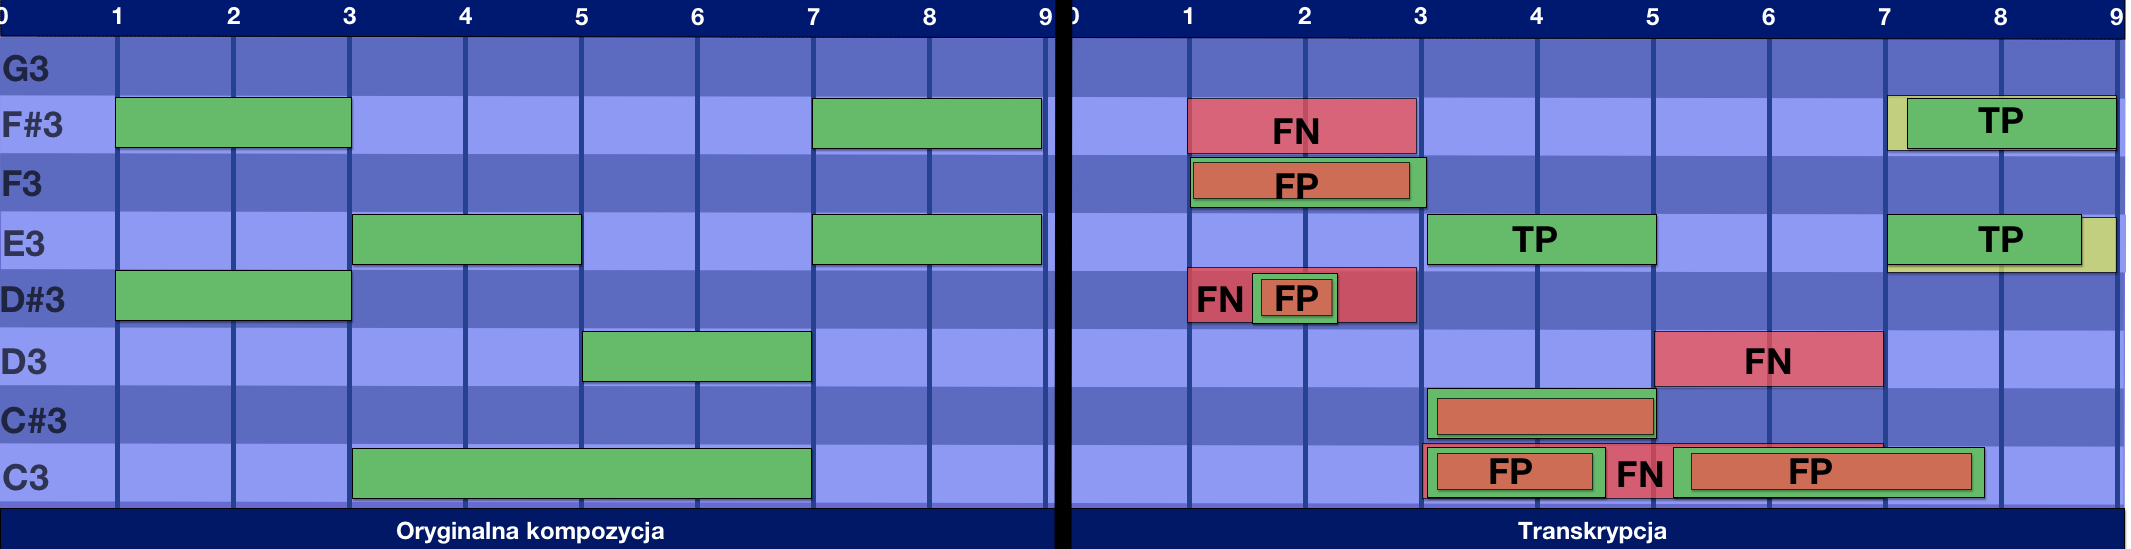
\includegraphics[scale=0.21]{images/TranscriptionStatisticF1Measure.jpg}
    \caption{Przykład rolki pianina dwóch plików MIDI. Utwór referencyjny (lewa rolka) przedstawia oryginalne rozłożenie nut. Na wyniku transkrypcji (prawa rolka) oznaczone są klasyfikacje statystyczne.}
    \label{fig:f1}
  \end{center}
\end{figure}

Funkcja porównująca przyjmuje jako argumenty maksymalny dozwolony błąd \textit{maxError} będący liczbą sekund dozwolonego offsetu pomiędzy porównywanymi zdarzeniami oraz dwie listy nut MIDI: \textit{transcriptionMidiNotes} będącą wynikiem ewaluowanego algorytmu i \textit{groundTruthMidiNotes} będącą oryginalną kompozycją. Działanie algorytmu można podzielić na trzy etapy:
\begin{enumerate}
  \item policzenie wszystkich FP poprzez sprawdzenie, czy dana nuta z tablicy \textit{transcriptionMidiNotes} posiada odpowiednik w tablicy \textit{groundTruthMidiNotes}. Dla każdej pozycji bez pary zwiększany jest licznik FP,
  \item policzenie wszystkich TP i FN poprzez sprawdzenie, czy dana nuta z tablicy \textit{groundTruthMidiNotes} posiada odpowiednik w tablicy \textit{transcriptionMidiNotes}. Gdy para zostanie znaleziona zwiększany jest licznik TP, w przeciwnym wypadku zwiększany jest licznik FN,
  \item policzenie miar statystycznych
\end{enumerate}
Szczegółowy opis wyliczanych miar statystycznych znajduje się w rozdziale \ref{sec:ewal}.

W celach porównawczych zostało również przeprowadzone sprawdzenie czasu wykonywania poszczególnych algorytmów transkrypcji. Zagadnienie to jest szczególnie ciekawe w kontekście porównania czasu wykonania algorytmów w wersji wykorzystujących GPU do tej wykonywanej w całości na CPU. Zaimplementowany dekorator \textit{profile} znajdujący się w pliku \textit{server/utils/custom\_profile.py} każdorazowo mierzy czas wywołania funkcji i zapisuje go. Wynik przedstawiany jest w postaci średniej ($\frac{\textrm{suma czasów}}{\textrm{ilość wywołań}}$) z wyłączeniem $n$ najwolniejszych i najszybszych wywołań w celu wykluczenia wartości skrajnych.

Podczas porównywania wyników algorytmów ważnym jest, aby dla każdego z nich dobrać parametry tak, aby wynikowe F1 było jak największe. Podczas gdy pojedyńczy parametr, jak np. długość okna, ma swoje odwzorowanie w manipulacji dokładności w dziedzinie czasu i częstotliwości, tak oszacowanie wektora optymalnych parametrów, z czego każdy może wpływać na pozostałe, nie jest tak trywialne. W celu znalezienia najlepszych argumentów zaimplementowanych algorytmów został napisany mechanizm, który iteruje po zbiorze kombinacji proponowanych argumentów i wylicza dla nich miarę F1 na podstawie zbioru walidacyjnego. 

W celu poprawnej interpretacji ewaluacji metody zostały podzielone na dwie grupy:
\begin{enumerate}
  \item przeznaczone jedynie dla sygnału monofonicznego
  \item przeznaczone zarówno dla sygnału monofonicznego jak i polifonicznego.
\end{enumerate}
Mechanizm porównujący wyniki algorytmów, którego implementacja znajduje się w pliku \textit{server/utils/evaluate.py}, wykonuje operacje opisane w tej sekcji dla wszystkich algorytmów według schematu poniżej:
\begin{enumerate}
  \item dla każdego algorytmu z badanej grupy wyznaczany jest wektor najlepszych argumentów na podstawie zbioru walidacyjnego (funkcja \textit{validate\_arguments}) i wszystkich kombinacji argumentów dla zadeklarowanych przyjmowanych wartości,
  \item dla każdego algorytmu badanej grupy wykonywana jest ewaluacja miar statystycznych i czasu wykonywania z wykorzystaniem zbioru testowego (funkcja \textit{run\_test\_on\_dataset\_with\_args}).
\end{enumerate}
Dane wejściowe, na których wykonywana jest ewaluacja deklarowane są jako zbiory danych opisane plikiem JSON. Każdy zbiór danych jest osobnym katalogiem w folderze \textit{server/test\_sounds/data\_sets} zawierającym:
\begin{itemize}
  \item plik o nazwie \textit{metadata.json}, w którym opisany jest zbiór danych. Każdy element musi zawierać cztery parametry:
  \begin{itemize}
    \item \textit{split} - deklaracja do jakiej grupy podziału należy dana pozycja. Wykorzystywane wartości to \textit{validation} (używane do wyznaczania najlepszych parametrów) i \textit{test} (używane do ewaluacji),
    \item \textit{midi\_filename} - relatywna względem katalogu zbioru danych ścieżka do pliku MIDI,
    \item \textit{audio\_filename} - relatywna względem katalogu zbioru danych ścieżka do pliku audio,
    \item \textit{canonical\_title} - nazwa kompozycji
  \end{itemize}
  \item plików audio i MIDI zgodnych z opisem w \textit{metadata.json}
\end{itemize}
Metody ewaluacyjne przyjmują nazwę zbioru danych, z którego mają być brane dane oraz generują kombinacje argumentów wejściowych na podstawie zadeklarowanych słowników \textit{argsAc}, \textit{argsAclos} itd. Ze względu na to, że złożoność obliczeniowa rośnie wykładniczo wraz ze wzrostem możliwych wartości argumentów, algorytmy te wykorzystują multi-procesowość w celu polepszenia czasu wykonywania (co widać na listingu \ref{code:eval:multiproces}). 

\begin{lstlisting}[language=Python, caption={Algorytm szukający najlepszej kombinacji argumentów dla zadanej funkcji func.}, captionpos=b, label={code:eval:multiproces}, numbers=none]
with concurrent.futures.ProcessPoolExecutor() as executor:
  processes = []
  bestF1 = 0
  bestArgs = None
  idx = 1
  for arg in possibleArgsCombinations:
      processes.append(executor.submit(validate_arguments, func, arg, evalObjects,
      saveRes, isResMidi, False, str(idx) + "/" + str(len(possibleArgsCombinations))))
      idx += 1
  for res in processes:
      currArg, currF1 = res.result()
      if currF1 > bestF1:
          bestF1 = currF1
          bestArgs = currArg

return currArg, bestF1
\end{lstlisting}

\subsection{Interfejs GUI}\label{sec:impl:gui}
W ramach projektu został zaimplementowany interfejs graficzny, na który składa się serwer HTTP napisany w języku python oraz strona napisana w języku \textit{TypeScript} i technologii \textit{React}. Daje ona możliwość wywołania każdej z wyżej opisanych implementacji algorytmów transkrypcji muzyki z wcześniej wyliczonymi optymalnymi parametrami.

Działanie serwera sprowadza się do implementacji przechwytywania zapytań od klienta i odsyłania wyniku pożądanego algorytmu w jednym z dwóch postaci:
\begin{enumerate}
  \item dla algorytmów przeznaczonych do analizy sygnałów monofonicznych - obiekt JSON, którego kluczami są nazwy poszczególnych wykresów (np. spektrogram, cepstrogram) a wartościami odpowiednie grafiki zakodowane do formatu Base64,
  \item dla algorytmy przeznaczonych do analizy sygnałów monofonicznych i polifonicznych - plik MIDI transkrypcji.
\end{enumerate} 
Implementacja serwera znajduje się w pliku \textit{server/server.py}.

Skrypty źródłowe graficznego interfejsu znajdują się w katalogu \textit{static/src} i służą do wygenerowania statycznej strony, która jest wysyłana przez serwer do przeglądarki klienta. Zbudowana paczka jest poddana procesowi minifikacji i składa się ze standardowych plików rozpoznawanych przez przeglądarki internetowe - \textit{css}, \textit{js} oraz \textit{html}. Opis uruchomienia pełnego GUI na lokalnej maszynie znajduje się w pliku \textit{README.md} w katalogu głównym projektu.

\newpage
\section{Ewaluacja} \label{sec:ewal}
W tym rozdziale opisane są wyniki ewaluacji zaimplementowanych w ramach pracy magisterskiej algorytmów. Proces ewaluacyjny polega na znalezieniu wektora najlepszych argumentów danej funkcji, a następnie porównaniu wyniku transkrypcji z oryginalną kompozycją dla każdego utworu ze zbioru testowego. Ewaluacja zaimplementowanych algorytmów została wykonana przy pomocy metod przedstawionych w sekcji \ref{sec:impl:midiCompare}. Użyte do testów dane pochodzą z bazy MAESTRO \cite{Transcription:Curtis:MAESTRO}. Wynik przedstawiony jest w postaci miary statystycznej F1, dokładności oraz średniego czasu wykonywania.

Na podstawie mocy sklasyfikowanych przez algorytmy ewaluacyjne zbiorów TP, FP i FN mierzone są cztery miary statystyczne:
\begin{itemize}
  \item dokładność (ang. \textit{accuracy}) pokazująca skale poprawnie wykrytych obserwacji na tle wszystkich sklasyfikowanych obserwacji (\ref{eq:acc}),
  \item precyzja (ang. \textit{precision}) pokazująca jaka część klasyfikacji dodatniej jest prawdziwie dodatnia (\ref{eq:percision}),
  \item czułość (ang. \textit{recall}) pokazująca jaka część spośród wszystkich dodatnich wyników została wykryta przez transkrypcję (\ref{eq:recall}),
  \item miara jakości F1 jako harmoniczna średnia precyzji i czułości (\ref{eq:f1}).
\end{itemize}

\begin{equation} \label{eq:acc}
  \textrm{accuracy} = \frac{TP}{TP + FP + FN}
\end{equation}
\begin{equation} \label{eq:percision}
  \textrm{precision} = \frac{TP}{TP + FP}
\end{equation}
\begin{equation} \label{eq:recall}
  \textrm{recall} = \frac{TP}{TP + FN}
\end{equation}
\begin{equation}  \label{eq:f1}
  F1 = 2 \cdot  \frac{\textrm{precision} \cdot  \textrm{recall}}{\textrm{precision} + \textrm{recall}}
\end{equation}

Do ewaluacji algorytmów analizujących sygnał monofoniczny została wydzielona część danych bazy MAESTRO, a następnie zmodyfikowane zostały pliki MIDI tak, aby w danym momencie w czasie obecna była tylko jedna nuta. Na podstawie tych plików zostały wygenerowane sygnały audio z wykorzystaniem sampli pianina Steinway. Dane podzielone są do grupy używanej w celu wyznaczenia najlepszych argumentów oraz do grupy, na której wykonywane są testy. Ewaluacja algorytmów analizujących sygnał polifoniczny została wykonana na części bazy MAESTRO wybranej w sposób losowy z uwzględnieniem podziału danych (grupy testowe i ewaluacyjne). Pozycje oryginalnie przypisane do zbioru ewaluacyjnego wykorzystane zostały do wyznaczenia najlepszych argumentów, natomiast te ze zbioru testowego były użyte do wyliczenia wyników. Testy obu przypadkach (dla sygnałów monofonicznych i polifonicznych) zostały wykonane na maszynie z procesorem Intel Core i5 3,19 GHz oraz kartą graficzną NVIDIA GeForce GTX 1060 3GB.

W tablicy \ref{tab:bestArgMono} przedstawione są argumenty zaimplementowanych funkcji użyte podczas procesu ewaluacji dla sygnałów monofonicznych (analogicznie tablica \ref{tab:bestArgPoli} dla sygnałów polifonicznych). Skrócone algorytmów symbolizują: 
\begin{itemize}
  \item AC - autokorelacja \ref{sec:f0:ac}
  \item ACLOS - autokorelacja na logarytmie widma \ref{sec:f0:aclos}
  \item CEPS - analiza cepstralna \ref{sec:f0:ceps}
  \item P\&I 08 - metoda Pertusa i Iñesta z 2008 \ref{sec:pertus1}
  \item P\&I 12 - metoda Pertusa i Iñesta z 2012 \ref{sec:petrus2}
\end{itemize}
Nazwy argumentów symbolizują:
\begin{itemize}
  \item NO - długość okna w samplach,
  \item odstęp - odstępy pomiędzy kolejnymi oknami,
  \item marg. zer - wymiar tablicy zer dodanej do okna przed wykonaniem FFT,
  \item W - ilość analizowanych sąsiednich nut przy scalaniu podczas przetwarzania końcowego,
  \item min/max F0 - odpowiednio minimalna / maksymalna częstotliwość jaka jest analizowana w kontekście F0 (w Hz),
  \item $P$ - minimalny odstęp pomiędzy pikami w amplitudzie (w samplach),
  \item $\mu$ - próg amplitudy, poniżej którego zerowane są wartości,
  \item $\eta$ - minimalna ilość harmonicznych dla kandydata F0,
  \item $\gamma$ - parametr sterujący maksymalną różnicą w parametrze głośności w kombinacji,
  \item $f_r$ - parametr sterujący maksymalną nieharmonicznością,
  \item C - maksymalna ilość równoległych dźwięków,
  \item lifter - mnożnik lifteringu. Dla wartości 0 funkcja lifteringu nie jest wykonywana,
  \item $k$ - ważność współczynnika gładkości,
  \item K - zakres wygładzania czasowego (w oknach czasowych),
  \item M - zakres śledzenia wysokości (w oknach czasowych).
\end{itemize}
Wartość ,,-'' oznacza, że parametr nie jest używany w danym algorytmie. Argumenty użyte podczas ewaluacji sygnałów polifonicznych są przedstawione w tablicy \ref{tab:bestArgPoli} z analogiczną konwencją nazewnictwa.

\begin{table}[H]
  \begin{center}
    \begin{tabular}{ |c|c|c|c|c|c| } 
    \hline
    algorytm & NO & odstęp & marg. zer & $W$ & min/max F0  \\
    \hline
    AC & 1024 & 1024 & - & 1 &  50/5500  \\
    ACLOS & 4096 & 1024 & 2048 & 3 & -  \\
    CEPS & 4096 & 1024 & 8192 & 3 &- \\
    P\&I 08 & 2048 & 512 & 8192 & 3 & 50/5500 \\
    P\&I 12 & 2048 & 512 & 12288 & 3 & 50/5500 \\
    \hline
  \end{tabular}
\end{center}


\begin{center}
  \begin{tabular}{ |c|c|c|c|c|c|c|c|c|c|c| } 
    \hline
    algorytm & $P$ & \textit{$\mu$} & $\eta$  & $\gamma$ & $f_r$ & C & lifter & $k$ & K & M\\
    \hline
    P\&I 08 & 8 & 2 & 1  & 0.1& 0.32 & 1 & 0 & - & - & -\\
    P\&I 12 & 8 & 4 & 1  & 0.1& 0.22 & 1 & 8 & 3 & 2 & 4\\
    \hline
    \end{tabular}
  \caption{Wektory najlepszych argumentów dla każdej funkcji transkrypcji dla sygnałów monofonicznych.}\label{tab:bestArgMono}
  \end{center}
\end{table}

\begin{table}[H]
  \begin{center}
    \begin{tabular}{ |c|c|c|c|c|c| } 
      \hline
      algorytm & NO & odstęp & marg. zer & $W$ & min/max F0  \\
      \hline
      P\&I 08 & 2048 & 512 & 8192 & 3 & 50/5500 \\
      P\&I 12 & 2048 & 512 & 12288 & 3 & 50/5500 \\
      \hline
    \end{tabular}
  \end{center}


  \begin{center}
    \begin{tabular}{ |c|c|c|c|c|c|c|c|c|c|c| } 
      \hline
      algorytm & $P$ & \textit{$\mu$} & $\eta$  & $\gamma$ & $f_r$ & C & lifter & $k$ & K & M\\
      \hline
      P\&I 08 & 8 & 2 & 1  & 0.1& 0.32 & 1 & 0 & - & - & -\\
      P\&I 12 & 8 & 4 & 1  & 0.1& 0.22 & 1 & 8 & 3 & 2 & 4\\
      \hline
      \end{tabular}
  \end{center}
  \caption{Wektory najlepszych argumentów dla funkcji transkrypcji dla sygnałów polifonicznych.}
  \label{tab:bestArgPoli}
\end{table}

Wyniki ewaluacji algorytmów dla sygnałów monofonicznych znajdują się w tabeli \ref{tab:eval:mono}. Testy wykonane zostały z maksymalnym błędem początku i trwania nuty równym 0.085 sekundy na 11 kompozycjach z łącznie 269 zdarzeniami MIDI i łącznym czasem odtwarzania 72s. Miary statystyczne są średnią miar wszystkich przypadków testowych. Kolumna T reprezentuje średni czas wykonania algorytmu. Kolumny FN, FP i TP odpowiadają mocy zbiorów wszystkich sklasyfikowanych zdarzeń. W celu uzyskania bardziej rzetelnego rezultatów czasu wykonania, wszystkie testy były wykonane dziesięciokrotnie i odrzuconych zostało 5 najszybszych i najwolniejszych wyników.

Cepstrum liczone na GPU jest wolniejsze od tego liczonego na CPU dlatego, że plan dla innych danych wejściowych musi być wyliczany w każdej iteracji. Dla przedstawienia realnego przyspieszenia, jakie daje użycie karty graficznej przy wyliczaniu cepstrum z sygnału, zostały wykonane dodatkowe testy w postaci 1000 powtórzeń analizy F0 algorytmem cepstrum z użyciem GPU i użyciem jedynie CPU dla pojedyńczego pliku dźwiękowego o czasie odtwarzania 38s. W tym teście, z odrzuceniem 10 skrajnych wyników, średni czas wykonywania algorytmu na samym CPU wyniosła  0.828s. podczas gdy algorytm wykonany z użyciem GPU osiągnął średni czas wykonywania równy 0.670s.

Wyniki ewaluacji algorytmów dla sygnałów polifonicznych znajdują się w tabeli \ref{tab:eval:poli}. Testy wykonane zostały z maksymalnym błędem początku i trwania nuty równym 0.085 sekundy na 2 kompozycjach z łącznie 4431 zdarzeniami MIDI i łącznym czasem odtwarzania 310s. Miary statystyczne są średnią miar wszystkich przypadków testowych, natomiast kolumna T reprezentuje średni czas wykonania algorytmu. Kolumny FN, FP i TP odpowiadają mocy zbiorów wszystkich sklasyfikowanych zdarzeń.

\begin{table}[H]
  \begin{center}
    \begin{tabular}{ |c|c|c|c|c|c|c|c|c| } 
    \hline
    algorytm & FN & FP & TP & dokładność & precyzja & czułość & F1 & T\\
    \hline
    AC & 106 & 229 & 163 & 0.326 & 0.380 & 0.515 & 0.425 & 3.96 \\
    ACLOS & 104 & 357 & 165 & 0.266 & 0.297 & 0.485 & 0.360 & 11.82\\
    CEPS & 83 & 487 & 186 & 0.279 & 0.309 & 0.647 & 0.400 & 0.42\\
    CEPS GPU & - & - & - & - & - & - & - & 1.97\\
    P\&I 08  & 112 & 198 & 157 & 0.337 & 0.430 & 0.484 & 0.443 & 4.31\\
    P\&I 12 & 142 & 284 & 127 & 0.225 & 0.308 & 0.367 & 0.320 & 5.54\\
    Onsets\&Frames & 122 & 158 & 147 & 0.299 & 0.360 & 0.401 & 0.379 & 9.452\\
    \hline
    \end{tabular}
  \end{center}
  \caption{Wyniki transkrypcji sygnałów monofonicznych}
  \label{tab:eval:mono}
\end{table}

\begin{table}[H]
  \begin{center}
      \begin{tabular}{ |c|c|c|c|c|c|c|c|c| } 
      \hline
      algorytm & FN & FP & TP & dokładność & precyzja & czułość & F1 & T\\
      \hline
      P\&I 08 & 1452& 16023& 2979& 0.157 & 0.142 & 0.663 & 0.233 & 5250.99\\
      P\&I 12 & 1748& 9198& 2683& 0.181 & 0.206 & 0.602 & 0.305 & 2675.14\\
      Onsets\&Frames & 4125& 3695& 306& 0.029 & 0.058 & 0.052 & 0.055& 40.50 \\
      \hline
      \end{tabular}
  \end{center}
  \caption{Wyniki transkrypcji sygnałów polifonicznych}
  \label{tab:eval:poli}
\end{table}


\newpage
\setcounter{secnumdepth}{0}
\section{Zakończenie} \label{sec:end}
W tej pracy magisterskiej przedstawiony został problem automatycznej transkrypcji muzyki wraz z metodologiami jego rozwiązania. W rozdziale \ref{sec:JakDzialaMuzyka} zdefiniowane zostały pojęcia teorii muzyki oraz jej cechy, jak i ich istotność w kontekście opisywanego tematu. Rozdział \ref{sec:modelowanieSystemu} przedstawił ogólne założenia transkrypcji muzyki wraz z szczegółowym opisem używanego w nich potężnego narzędzia matematycznego jakim jest transformata Fouriera. Rozdziały \ref{sec:f0} i \ref{sec:MultiPitch} opisują wybrane algorytmy do wykrywania wysokości F0 w odpowiednio sygnale monofonicznym i sygnale polifonicznym. Kod, który powstał w ramach tej pracy implementuje przedstawione metody i jest opisany w rozdziale \ref{sec:impl}. Zaimplementowane zostały również funkcję ewaluacyjne, które porównują omawiane algorytmy pod względem jakości wyniku miarą F1 oraz mierzą ich czas wykonania. Opis ewaluacji zaimplementowanych metod transkrypcji muzyki opisany jest w rozdziale \ref{sec:ewal}.

Znacząca część pracy skupia się jedynie na problemie częściowym transkrypcji muzyki jakim jest wykrycie wysokości obecnych w sygnale dźwięków. Pozostałe problemy, jak analiza rytmiki czy barwy dźwięku została jedynie przedstawiona, bez dogłębnej analizy. Przedstawione metodologie pokazują, że zadanie transkrypcji muzyki jest złożonym tematem przetwarzania sygnałów, który nie ma jednego optymalnego rozwiązania. Opisane algorytmy zakładają kompozycje przestrzegającą zasad muzyki zachodniej, co jest istotnym ograniczeniem możliwych danych wejściowych. 

Polifoniczność w sygnale jest czynnikiem, który najmocniej wpływa na złożoność problemu transkrypcji muzyki. Rozróżnienie poszczególnych równoległych dźwięków wykonywane jest przy pomocy różnych metod, które często łączone są w złożone algorytmy, jak w metodach Metoda Pertusa i Iñesta \ref{sec:pertus1} \ref{sec:petrus2}. Inną próbą transkrypcji polifonii jest wykrywanie wzorców w sygnale, co ma miejsce w algorytmach bazujących na uczeniu maszynowym. Przykładami takich rozwiązań są \textit{Onsets and Frames} i holistyczna metoda Pertusa, opisane w odpowiednio \ref{sec:multif0:onsetsAndFrames} i \ref{sec:multif0:petrusNetwork}.

W dniu pisania pracy nie istnieje rozwiązanie omawianego problemu dla uniwersalnych danych wejściowych. Co więcej, nie istnieje bezbłędne system transkrypcji nawet dla kompozycji z ograniczeniem do standardów muzyki zachodniej i użycia pojedyńczego instrumentu, jakim jest pianino. Analiza wyników algorytmów pokazuje jednak, że wraz z nowymi rozwiązaniami na przestrzeni lat osiągane są nowe rekordy pod względem jakości wyników algorytmów transkrypcji muzyki. 

% TODO: Czy słownik skrótów potrzebny? Cheng-Zhi A. Huang -> C.A.Huang ?  Same Hirsch, Hans-Günter, Biing-Hwang

%%\TODO: Jak przetłumaczyć ,,Gaussian smoothnes''? W tekscie dałem "gładkość Gaussa", ale nie jestem pewny czy to poprawne. Ten sam problem z oknem Gaussa / oknem Gaussiana. Średnia Gaussowska czy Średnia Gaussa? Nazwałem "równoległych metod" nazwę "joint methods". Dosłownie byłoby to "Wspólnych metod", ale ich działanie de facto polega na wyliczaniu równoległym a nie iteracyjnym. Czy to jest ok? }
%TODO: Czy opisywać funkcje kosztu w rozdziale Onsets and Frames? jest dokładnie opisana w referencyjnej pracy naukowej
%\TODO: [Holistyczna metoda z użyciem sieci neuronowych] Artykuł znajduje się na 20-30 stronach journala, ale sam w sobie numerowany jest od 1 - 10. Jak odnoszę się do 6 strony, powinno to być 6 czy zgodnie z journalem 26? ten sam problem w fig:specSmooth:kapuri

% \section{Słownik skrótów}
% \begin{itemize}
%   \item \textbf{FT} - \textit{ang. \textbf{F}ourier \textbf{T}ransform}, pol. Transformata Fouriera
%   \item \textbf{DFT} - \textit{ang. \textbf{D}iscrete \textbf{F}ourier \textbf{T}ransform}, pol. Dyskretna Transformata Fouriera
%   \item \textbf{FFT} - \textit{ang. \textbf{F}ast \textbf{F}ourier \textbf{T}ransform}, pol. Szybka Transformata Fouriera
%   \item \textbf{STFT} - \textit{ang. \textbf{S}hort- \textbf{T}ime \textbf{F}ourier \textbf{T}ransform}, pol. Krótkoczasowa Transformata Fouriera
%   \item \textbf{DAW} - \textit{ang. \textbf{D}igital \textbf{A}udio \textbf{W}orkstation}, pol. Cyfrowa Stacja Robocza 
%   \item \textbf{MIDI} - \textit{ang. \textbf{M}usical \textbf{I}nstrument \textbf{D}igital \textbf{I}nterface}, pol. Cyfrowy Interfejs Instrumentów Muzycznych
%   \item \textbf{AUX} - \textit{ang. \textbf{Aux}iliary}
%   \item \textbf{W3C} - \textit{ang. \textbf{W}orld \textbf{W}ide \textbf{W}eb \textbf{C}onsortium}
%   \item \textbf{HTML} - \textit{ang. \textbf{H}yper\textbf{t}ext \textbf{M}arkup \textbf{L}anguage}
%   \item \textbf{CSS} - \textit{ang.  \textbf{C}ascading \textbf{S}tyle \textbf{S}heets}
%   \item \textbf{JS} - \textit{\textbf{J}ava\textbf{S}cript}
%   \item \textbf{TS} - \textit{\textbf{T}ype\textbf{S}cript}
%   \item \textbf{DOM} - \textit{ang. \textbf{D}ocument \textbf{O}bject \textbf{M}odel}
%   \item \textbf{API} - \textit{ang. \textbf{A}pplication \textbf{P}rogramming \textbf{I}nterface}
%   \item \textbf{CLI} - \textit{ang. \textbf{C}ommand \textbf{L}ine \textbf{I}nterface}
%   \item \textbf{CQRS} - \textit{ang. \textbf{C}ommand \textbf{Q}uery \textbf{R}esponsibility \textbf{S}egregation}
%   \item \textbf{URL} - \textit{ang. \textbf{U}niform \textbf{R}esource \textbf{L}ocator }
%   \item \textbf{npm} - \textit{ang. \textbf{N}ode \textbf{P}ackage \textbf{M}anager}
%   \item \textbf{IOI} - \textit{ang. \textbf{I}nter-\textbf{o}nset \textbf{i}nterval, pol. Odstęp pomiędzy początkami dźwięków}
%   \item \textbf{TFR} - \textit{ang. \textbf{T}ime-\textbf{F}requency \textbf{R}epresentation, pol. Reprezentacja Czasu-Częstotliwości}
%   \item \textbf{AMT} - \textit{ang. \textbf{A}utomatic \textbf{M}usic \textbf{T}ranscription}
%   \item \textbf{HPS} - \textbf{H}ypothetical \textbf{P}artial \textbf{S}equences - hipotetyczne częściowe sekwencje
%   \item \textbf{wDAG} - weighted \textbf{D}irected \textbf{A}cyclic \textbf{G}raph
%   \item \textbf{MPS} - \textbf{M}ulti- \textbf{P}itch \textbf{S}treaming
%   \item \textbf{NN} - Neural Network
%   \item \textbf{MIREX} - The Music Information Retrieval Evaluation eXchange
%   \item \textbf{A2S} - Audio=to-Score
%   \item \textbf{LSTM}
%   \item \textbf{MAESTRO} - “MIDI and Audio Edited for Synchronous TRacks and Organization”
%   \item \textbf{GUI}
%   \item \textbf{GPU}
% \end{itemize}

\clearpage
\BeginNoToc
\listoffigures
\EndNoToc
\addcontentsline{toc}{section}{Spis rysunków}

\newpage

\BeginNoToc
\listoftables
\EndNoToc
\addcontentsline{toc}{section}{Spis tablic}
\newpage
\cleardoublepage
\lstlistoflistings
\addcontentsline{toc}{section}{Spis listingów}

\newpage
\printbibliography

\end{document}  
